%%%%%%%%%%%%%%%%%%%%%%%%%%%%%%%%%%%%%%%%%%%%%%%%%%%%%%%%%%%%%%%%%%%%
%%%%%%%%%%%%%%%%%%%%%%%%%%%%%%%%%%%%%%%%%%%%%%%%%%%%%%%%%%%%%%%%%%%%
%%                                                                %%
%% Esimerkki opinnäytteen tekemisestä LaTeX:lla 20130926          %%
%% Alkuperäinen versio Luis Costa,  muutokset Perttu Puska        %%
%%                                                                %%
%% Tähän esimerkkiin kuuluu tiedostot                             %%
%%               opinnaytepohja.tex (versio 1.7)                  %%
%%               aaltothesis.sty (versio 1.7)                     %%
%%               kuva1.eps                                        %%
%%               kuva2.eps                                        %%
%%                                                                %%
%%                                                                %%
%% Kääntäminen                                                    %%
%% latex:                                                         %%
%%             $ latex opinnaytepohja                             %%
%%             $ latex opinnaytepohja                             %%
%%                                                                %%
%%   Tuloksena on tiedosto opinnayte.dvi, joka                    %%
%%   muutetaan ps-muotoon seuraavasti                             %%
%%                                                                %%
%%             $ dvips opinnaytepohja -o                          %%
%%                                                                %%
%% Selittävät kommentit on tässä esimerkissä varustettu           %%
%% %%-merkeillä ja muutokset, joita käyttäjä voi tehdä,           %%
%% on varustettu %-merkeillä                                      %%
%%                                                                %%
%%%%%%%%%%%%%%%%%%%%%%%%%%%%%%%%%%%%%%%%%%%%%%%%%%%%%%%%%%%%%%%%%%%%
%%%%%%%%%%%%%%%%%%%%%%%%%%%%%%%%%%%%%%%%%%%%%%%%%%%%%%%%%%%%%%%%%%%%

%% Käytä toinen näistä, jos kirjoitat suomeksi:
%% ensimmäinen, jos käytät pdflatexia (kuvat on oltava pdf-tiedostoina)
%% toinen, jos haluat tuottaa ps-tiedostoa (käytä eps-formaattia kuville).
%%
%% Use one of these you write in Finnish:
%% the 1st when using pdflatex (use pdf figures) or
%% the 2nd when producing a ps file (use eps figures).
%\documentclass[finnish,12pt,a4paper,pdftex]{article}
%\documentclass[finnish,12pt,a4paper,dvips]{article}


%% Käytä näitä, jos kirjoitat englanniksi
%%
%% Uncomment one of these if you write in English
\documentclass[english,12pt,a4paper,pdftex]{article}
%\documentclass[english,12pt,a4paper,dvips]{article}

%% Tämä paketti on pakollinen
%% Valitse korkeakoulusi näistä: arts, biz, chem, elec, eng, sci.
%% Valiste editorisi käyttämä merkkikoodaustapa: utf8, latin1
%%
%% This package is required
%% Choose your school from arts, biz, chem, elec, eng, sci.
%% Choose the character encoding scheme used by your editor: utf8, latin1
\usepackage[elec,utf8]{aaltothesis} % this is the default in aaltothesis.sty
%\usepackage[elec,latin1]{aaltothesis}

\usepackage[english]{babel}

%% Jos käytät latex-komentoa käännettäessä (oletusarvo), 
%% kuvat kannattaa tehdä eps-muotoon. Älä käytä ps-muotoisia kuvia!
%% Käytä seuraavaa latex-komennon ja eps-kuvien kanssa 
%%
%% Jos taas käytät pdflatex-komentoa, joka kääntää tekstin suoraan
%% pdf-tiedostoksi, kuvasi on oltava jpg-formaatissa tai pdf-formaatissa.
%%
%% Use this if you run pdflatex and use jpg/pdf-format pictures.
%%
\usepackage{graphicx}
\usepackage{float}
\usepackage{caption}
\usepackage{subcaption}
\usepackage{pdflscape}
\usepackage{afterpage}
\usepackage{rotating}
\usepackage{rotfloat}
\usepackage{verbatim}

\usepackage{lipsum}

%% Jos et jostain syystä pidä, miten alla oleva hyperref-paketti käyttää
%% fontteja, värejä yms., käytä tämän paketin makroja muuttamaan
%% fonttimäärittelyt. Katso paketin dokumentaatiota. Paketti määrittelee
%% \url-makron, joten ota paketti käyttöön, jos et käytä hyperref-pakettia.
%%
%% Use the macros in this package to change how the hyperref package below 
%% typesets its hypertext -- hyperlink colour, font, etc. See the package
%% documentation. It also defines the \url macro, so use the package when 
%% not using the hyperref package.

%\usepackage[sort&compress]{natbib}
\usepackage[normalem]{ulem}


\usepackage{xpatch}

\usepackage{csquotes}
\usepackage[style=ieee,sorting=none,sortcites=true,backend=biber]{biblatex}
%\usepackage[style=chem-acs,backend=biber,biblabel=brackets]{biblatex}
\addbibresource{references.bib}
\DefineBibliographyStrings{english}{phdthesis = {Doctoral dissertation}}

\xpatchbibdriver{online}
  {\printtext[parens]{\usebibmacro{date}}}
  {\iffieldundef{year}
    {}
    {\printtext[parens]{\usebibmacro{date}}}}
  {}
  {\typeout{There was an error patching biblatex-ieee (specifically, ieee.bbx's @online driver)}}



\usepackage{enumitem}
\setlist{nolistsep}

\usepackage{array}
\usepackage{multirow}
%\newcolumntype{P}[1]{>{\centering\arraybackslash}p{#1}}
%\newcolumntype{M}{>{\centering\arraybackslash}m{\dimexpr.25\linewidth-2\tabcolsep}}
\newcolumntype{M}[1]{>{\centering\arraybackslash}m{#1}}

%% Saat pdf-tiedoston viittaukset ja linkit kuntoon seuraavalla paketilla.
%% Paketti toimii erityisen hyvin pdflatexin kanssa. 
%%
%% Use this if you want to get links and nice output with pdflatex
\usepackage[pdfpagemode=None,colorlinks=true,urlcolor=black,%
linkcolor=black,citecolor=black,pdfstartview=FitH]{hyperref}
\usepackage{breakurl}

\usepackage{cleveref}
\newcommand{\crefrangeconjunction}{--}

%% Matematiikan fontteja, symboleja ja muotoiluja lisää, näitä tarvitaan usein 
%%
%% Use this if you write hard core mathematics, these are usually needed
\usepackage{amsfonts,amssymb,amsbsy,mathtools}
\usepackage[amssymb]{SIunits}
\newcommand\sub[2]{{#1}_{\mathrm{#2}}}
\renewcommand\j{\mathrm{j}}
\newcommand\db{\mathrm{dB}}

\usepackage{textcomp}

\usepackage{tikz}
\usepackage[american]{circuitikz}
\tikzstyle{densely dashed}= [dash pattern=on 4pt off 3pt]
\usetikzlibrary{decorations.pathreplacing,decorations.pathmorphing}

%% Vaakasuunnan mitat, ÄLÄ KOSKE!
\setlength{\hoffset}{-1in}
\setlength{\oddsidemargin}{35mm}
\setlength{\evensidemargin}{25mm}
\setlength{\textwidth}{15cm}
%% Pystysuunnan mitat, ÄLÄ KOSKE!
\setlength{\voffset}{-1in}
\setlength{\headsep}{7mm}
\setlength{\headheight}{1em}
\setlength{\topmargin}{25mm-\headheight-\headsep}
\setlength{\textheight}{23cm}


%% Kaikki mikä paperille tulostuu, on tämän jälkeen
%%
%% Output starts here
\begin{document}

%% Korjaa vastaamaan korkeakouluasi, jos automaattisesti asetettu nimi on 
%% virheellinen 
%%
%% Change the school field to describe your school if the autimatically 
%% set name is wrong
% \university{aalto University}{aalto-Yliopisto}
% \school{School of Electrical Engineering}{SähköTekniikan korkeakoulu}

%% Vain kandityölle: Korjaa seuraavat vastaamaan koulutusohjelmaasi
%%
%% Only for B.Sc. thesis: Choose your degree programme. 
%\degreeprogram{Electronics and electrical engineering}%
%{Elektroniikka ja sähkötekniikka}
%%

%% Vain DI/M.Sc.- ja lisensiaatintyölle: valitse laitos, 
%% professuuri ja sen professuurikoodi. 
%%
%% Only for M.Sc. and Licentiate thesis: Choose your department,
%% professorship and professorship code. 
\department{Department of Radio Science and Technology}%
{Radiotieteen ja -tekniikan laitos}
\professorship{Radio Science and Engineering}{Radiotiede ja -tekniikka}
\code{S-26}
%%

%% Valitse yksi näistä kolmesta
%%
%% Choose one of these:
%\univdegree{BSc}
\univdegree{MSc}
%\univdegree{Lic}

%% Oma nimi
%%
%% Should be self explanatory...
\author{Joni Kurvinen}

%% Opinnäytteen otsikko tulee vain tähän. Älä tavuta otsikkoa ja
%% vältä liian pitkää otsikkotekstiä. Jos latex ryhmittelee otsikon
%% huonosti, voit joutua pakottamaan rivinvaihdon \\ kontrollimerkillä.
%% Muista että otsikkoja ei tavuteta! 
%% Jos otsikossa on ja-sana, se ei jää rivin viimeiseksi sanaksi 
%% vaan aloittaa uuden rivin.
%% 
%% Your thesis title. If the title is very long and the latex 
%% does unsatisfactory job of breaking the lines, you will have to
%% break the lines yourself with \\ control character. 
%% Do not hyphenate titles.
\thesistitle{Antennas for metal-covered handsets}{Metallikuoristen matkapuhelimien antennit}

\place{Espoo}
%% Kandidaatintyön päivämäärä on sen esityspäivämäärä! 
%% 
%% For B.Sc. thesis use the date when you present your thesis. 
\date{xy.qw.2016}

%% Kandidaattiseminaarin vastuuopettaja tai diplomityön valvoja.
%% Huomaa tittelissä "\" -merkki pisteen jälkeen, 
%% ennen välilyöntiä ja seuraavaa merkkijonoa. 
%% Näin tehdään, koska kyseessä ei ole lauseen loppu, jonka jälkeen tulee 
%% hieman pidempi väli vaan halutaan tavallinen väli.
%%
%% B.Sc. or M.Sc. thesis supervisor 
%% Note the "\" after the comma. This forces the following space to be 
%% a normal interword space, not the space that starts a new sentence. 
\supervisor{Prof.\ Ville Viikari}{Prof.\ Ville Viikari}

%% Kandidaatintyön ohjaaja(t) tai diplomityön ohjaaja(t)
%% 
%% B.Sc. or M.Sc. thesis advisor(s). 
%%
%% Note that there has been a change in the official EN translation
%% of the Finnish title ``ohjaaja'' which in the previous version (1.5) 
%% of this document was called ``instructor''. The recommended
%% translation is now ``advisor''.  
%% However, the LaTeX internal variable remains \instructor
%% as there is little point to change the variable name. 
%%
%\instructor{Prof. Pirjo Professori}{Prof. Pirjo Professori}
\instructor{D.Sc.\ (Tech.) Anu Lehtovuori}{TkT Anu Lehtovuori}
%\instructor{M.Sc.\ (Tech.) Polli Pohjaaja}{DI Polli Pohjaaja}

%% Aaltologo: syntaksi:
%% \uselogo{aaltoRed|aaltoBlue|aaltoYellow|aaltoGray|aaltoGrayScale}{?|!|''}
%% Logon kieli on sama kuin dokumentin kieli
%%
%% Aalto logo: syntax:
% \uselogo{aaltoRed|aaltoBlue|aaltoYellow|aaltoGray|aaltoGrayScale}{?|!|''}
%% Logo language is set to be the same as the document language.
\uselogo{aaltoRed}{?}

%% Tehdään kansilehti
%%
%% Create the coverpage
\makecoverpage

%
%% English abstract, uncomment if you need one. 
%% 
%% Abstract keywords
\keywords{Resistor, Resistance,\\ Temperature}
%% Abstract text
\begin{abstractpage}[english]
 Your abstract in English. Try to keep the abstract short, approximately 
 100 words should be enough. Abstract explains your research topic, 
 the methods you have used, and the results you obtained.  
\end{abstractpage}

%% Pakotetaan uusi sivu varmuuden vuoksi, jotta 
%% mahdollinen suomenkielinen ja englanninkielinen tiivistelmä
%% eivät tule vahingossakaan samalle sivulle
%%
%% Force new page so that English abstract starts from a new page
\newpage
%% Suomenkielinen tiivistelmä
%% 
%% Finnish abstract
%%
%% Tiivistelmän avainsanat
\keywords{Avainsanoiksi valitaan kirjoituksen sisältöä keskeisesti kuvaavia
käsitteitä}
%% Tiivistelmän tekstiosa
\begin{abstractpage}[finnish]
  Tiivistelmässä on lyhyt selvitys (noin 100 sanaa)
  kirjoituksen tärkeimmästä sisällöstä: mitä ja miten on tutkittu,
  sekä mitä tuloksia on saatu. 
  Tiivistelmässä on lyhyt selvitys (noin 100 sanaa)
  kirjoituksen tärkeimmästä sisällöstä: mitä ja miten on tutkittu,
  sekä mitä tuloksia on saatu. 

  Tiivistelmässä on lyhyt selvitys (noin 100 sanaa)
  kirjoituksen tärkeimmästä sisällöstä: mitä ja miten on tutkittu,
  sekä mitä tuloksia on saatu. 
  Tiivistelmässä on lyhyt selvitys (noin 100 sanaa)
  kirjoituksen tärkeimmästä sisällöstä: mitä ja miten on tutkittu,
  sekä mitä tuloksia on saatu. 
  Tiivistelmässä on lyhyt selvitys (noin 100 sanaa)
  kirjoituksen tärkeimmästä sisällöstä: mitä ja miten on tutkittu,
  sekä mitä tuloksia on saatu. 
\end{abstractpage}

%% Note that 
%% if you are writing your master's thesis in English place the English
%% abstract first followed by the possible Finnish abstract

%% Esipuhe 
%%
%% Preface
%\mysection{Esipuhe}
\mysection{Preface}
{\parindent0pt
Haluan kiittää Professori Pirjo 
Professoria ja ohjaajaani Olli Ohjaajaa hyvästä ja 
huonosta ohjauksesta.\\

Iuvenis in Aeternum.}

\vspace{5cm}
Tekniikan kehdossa, xy.qw.2016

\vspace{5mm}
{\hfill Joni Kurvinen \hspace{1cm}}

%% Pakotetaan varmuuden vuoksi esipuheen jälkeinen osa
%% alkamaan uudelta sivulta
%%
%% Force new page after preface
\newpage


%% Sisällysluettelo
%% 
%% Table of contents. 
\thesistableofcontents


%% Symbolit ja lyhenteet
%%
%% Symbols and abbreviations
%\mysection{Symbolit ja lyhenteet}
\mysection{Symbols and abbreviations}
%\subsection*{Symbolit}
\subsection*{Symbols}

\begin{tabular}{ll}

%$\mathbf{B}$  & density of magnetic flux  \\
$c$           & speed of light $\approx 3\times10^8\,\meter/\second$\\
$C$           & capacitance\\
$D(\theta,\phi)$  & directivity at direction ($\theta,\phi$)\\
$\sub{D}{max}$    & maximum directivity\\
$E_\theta$   & $\theta$-component of electric field\\
$f$          & frequency\\
$f(\theta,\phi)$ & pattern factor\\
$F(\theta,\phi)$ & (normalized) radiation pattern\\
$g(\theta,\phi)$ & element factor\\
$G(\theta,\phi)$ & gain at direction ($\theta,\phi$)\\
$G$          & gain\\
$L$          & inductance\\
$l$          & antenna length\\
$l_i$        & antenna length of element $i$\\
$\sub{P}{in}$     & input power\\
$\sub{P}{rad}$    & radiated power\\
$Q$          & quality factor\\
$R$          & resistance\\
$R_o$        & ohmic losses\\
$R_r$        & radiation resistance\\
$R_s$        & source resistance\\
$S_{ij}$     & scattering parameter to port $i$ from port $j$ \\
$w$          & antenna width\\
$X_a$        & antenna reactance\\
$X_s$        & source reactance\\
$x$          & Cartesian $x$-coordinate\\
$y$          & Cartesian $y$-coordinate\\
$Z_a$        & antenna impedance\\
$Z_s$        & source impedance\\
$z$          & Cartesian $z$-coordinate\\
& \\
$\Gamma$     & reflection coefficient\\
$\sub{\eta}{rad}$ & radiation efficiency \\
$\lambda_0$  & free space wavelength\\
$\phi$       & azimuth angle\\
$\rho_e$     & envelope correlation coefficient\\
$\theta$     & elevation angle\\


\end{tabular}

%\subsection*{Operaattorit}
%\subsection*{Opetators}

%\begin{tabular}{ll}
%$\nabla \times \mathbf{A}$              & vektorin $\mathbf{A}$ roottori\\
%$\displaystyle\frac{\mbox{d}}{\mbox{d} t}$ & derivaatta muuttujan $t$ suhteen\\
%[3mm]
%$\displaystyle\frac{\partial}{\partial t}$  & osittaisderivaatta muuttujan $t$ suhteen \\[3mm]
%$\sum_i $                       & Summa indeksin $i$ yli\\
%$\mathbf{A} \cdot \mathbf{B}$    & vektorien $\mathbf{A}$ ja $\mathbf{B}$ pistetulo
%\end{tabular}

%\subsection*{Lyhenteet}
\subsection*{Abbreviations}

\begin{tabular}{ll}
%AC         & alternating current \\
3G          & Third generation mobile network \\
3GPP        & Third Generation Partnership Project \\
4G          & Fourth generation mobile network \\
%CA         & Carrier aggregation \\
CCE         & Capacitive coupling element\\
CDMA        & Code Division Multiple Access \\
CEPT        & European Conference of Postal and \\
            & Telecommunications Administrations \\
DTC         & Digitally tunable capacitor\\
ECC         & Envelope correlation coefficient\\
EDGE        & Enhanced Data rates for GSM Evolution \\
EM          & Electromagnetic\\
ESA         & Electrically small antenna\\
ETSI        & European Telecommunications Standards Institute\\
FDD         & Frequency Division Duplexing \\
FDMA        & Frequency Division Multiple Access \\
GPRS        & General Packet Radio Service \\
GPS         & Global Positioning System \\
GSM         & Global System for Mobile communications \\
            & (originally Groupe Spécial Mobile) \\
HSPA        & High-Speed Packet Access \\
IFA         & Inverted F antenna\\
ILA         & Inverted L antenna\\
IMT-2000    & International Mobile Telecommunications for year 2000 \\
IMT-Advanced & International Mobile Telecommunications Advanced \\
ITU         & International Telecommunications Union \\
LTE         & Long-Term Evolution \\
LTE-Advanced & Long-Term Evolution Advanced\\
MIMO        & Multiple Input Multiple Output \\
MSA         & Microstrip antenna\\
OFDM        & Orthogonal Frequency Division Multiplexing \\
OFDMA       & Orthogonal Frequency Division Multiple Access\\
PCB         & Printed circuit board\\
PEC         & Perfect electric conductor\\
PIFA        & Planar inverted F antenna\\
PILA        & Planar inverted L antenna\\
RFID        & Radio Frequency Identification \\
Rx          & Receiver \\
SNR         & Signal-to-Noise Ratio \\
TD-SCDMA    & Time Division Synchronous Code Division Multiple Access \\
TDD         & Time Division Duplexing \\
TDMA        & Time Division Multiple Access \\
Tx          & Transmitter \\
UMTS        & Universal Mobile Telecommunication System \\
WCDMA       & Wideband Code Division Multiple Access \\
Wi-Fi       & Wireless Fidelity \\
WLAN        & Wireless Local Area Network \\
WWAN        & Wireless Wide Area Network\\
%TEM        & transverse electromagnetic
\end{tabular}


%% Sivulaskurin viilausta opinnäytteen vaatimusten mukaan:
%% Aloitetaan sivunumerointi arabialaisilla numeroilla (ja jätetään
%% leipätekstin ensimmäinen sivu tyhjäksi, 
%% ks. alla \thispagestyle{empty}).
%% Pakotetaan lisäksi ensimmäinen varsinainen tekstisivu alkamaan 
%% uudelta sivulta clearpage-komennolla. 
%% clearpage on melkein samanlainen kuin newpage, mutta 
%% flushaa myös LaTeX:n floatit 
%% 
%% Corrects the page numbering, there is no need to change these
\cleardoublepage
\storeinipagenumber
\pagenumbering{arabic}
\setcounter{page}{1}


%% Leipäteksti alkaa
%%
%% Text body begins. Note that since the text body
%% is mostly in Finnish the majority of comments are
%% also in Finnish after this point. There is no point in explaining
%% Finnish-language specific thesis conventions in English.
%\section{Johdanto}
\section{Introduction}
\label{sec:introduction}

%% Ensimmäinen sivu tyhjäksi
%% 
%% Leave first page empty
\thispagestyle{empty}

\begin{comment}
\begin{itemize}
\item[--]Tutkimuksen taustaa ja tutkimusaiheen yleisluonteinen esittely
\item[--]Tutkimuksen tavoitteet
\item[--]Pääkysymys ja osaongelmat
\item[--]Tutkimuksen rajaus ja keskeiset käsitteet.
\item[--]Työn rakenne
\end{itemize}
\end{comment}

The use of mobile devices have been growing rapidly for the last two decades, and the same trend will continue in the near future, as the global amount of mobile subscriptions is constantly increasing and applications are more and more data intensive \cite{nokia,cisco,ericsson,gsma}. Mobile phones are not anymore used for only traditional calls, but for communicating through a numerous different messaging services, social media, and other applications. Prior to the third generation mobile networks (3G), this have been impossible. 3G enlarged the channel bandwidth by factor of 25 \cite{molisch}, which enabled significantly higher data rates.

After 3G, the standards of mobile communications have kept on evolving, as new applications and demands have been invented. In 2008, International Telecommunications Union (ITU) announced the new requirements for mobile networks \cite{itur}. Long Term Evolution (LTE), or the fourth generation mobile networks (4G), would again multiply channel bandwidth and data rates to answer the need for faster networks. However, LTE does not fulfill the specifications, but its successor LTE-Advanced will. 4G networks use over 40 frequency bands around the world \cite{radio_electronics,molisch}, and provide 1\,Gb/s peak data transmission by utilizing techniques such as multiple input multiple output (MIMO) and carrier aggregation \cite{parkvall_lte}.

While the network standards have developed a lot, same time the mobile phones have changed their shapes several times \cite{anguera2}. Nowadays smartphones with large touch screens are the common device. Large displays reserve a major amount of space for themselves, which sets different constraints for the placement of other subsystems. Modern mobile phones operate already on a wide range of frequencies, and it is estimated that the amount of communications systems might exceed 20 in the future \cite{20ant}. This would mean 20 different antennas in a single device, which is quite a challenge for designers, as the network standards also demand a certain performance. To meet the requirements antennas should operate on multiple bands or support wideband communications \cite{lehtovuori_wideband_match}.

Fortunately, antenna techniques are developing together with the networks. From long monopoles and dipoles sticking outside the handset, the antennas are currently inside the phone, or integrated to the housing of the device \cite{saunders,molisch}. Different forms of planar antennas have been a popular choice, since they are able to operate on multiple bands \cite{anguera}. Although antennas are designed to operate on multiple bands, their size and shape might become uncontrollable, which restricts performance. A potential option is a capacitive coupling element (CCE), which can be used at a wide band, requires a smaller area, and typically has a simple structure \cite{valkonen_cce2}.

Modern networks and handheld devices ensure that mobility of people is not an obstacle for communicating with others anymore. Smart phones have become the main communication tools due to their rather compact size, light weight, and mechanical robustness. For improved strength and also better aesthetics, phone manufacturers have started to use metal covers and side frames \cite{rowell}. Metal covers and rims as conductive materials increase the size of the device's ground plane, which restricts the free space around the antennas. Close proximity of highly conductive materials also leads to narrower bandwidth and decreased efficiency \cite{rowell}. Antennas radiate poorly when enclosed by metal covers, as the structure resembles a small Faraday cage. To resolve this problem, phone manufacturers have started to integrate antennas straight into the metallic structures. For example, Apple's iPhone~4 among the first released metal-rimmed phones, has its antennas integrated into the rim. 

Only days after the release of iPhone~4, Apple received a lot of complaints about connectivity issues, and their first solution was to hold the phone differently \cite{apple_press,apple_bbc}. This solution clearly is not sustainable in the long run, and antenna designers are required to come up with new ideas for the future handsets. After iPhone~4, many other companies have released their metal-rimmed, or even metal-covered phones. Typical antenna has still been integrated to the structure, and it is usually separated from the other structures with a slot. In case of metal-covered phones, some slots are typically included to the back cover to improve the antenna performance. 

This thesis focuses on metal-covered phones. Moreover, the main purpose is to design antennas for mobile phone that has a slotless and continuous metal plate as a back cover. The thesis is part of a research project with AAC Technologies \cite{aac}, the specifications for the antennas are defined by the project. The detailed requirements for the antennas are specified in Section \ref{sec:objectives}. Briefly, the cellular antennas should be efficient, support MIMO and cover a wide range of frequencies. Additionally, the phone should have antennas for Wi-Fi (trademark for Wireless Local Area Networks (WLAN)), and Global Positioning System (GPS). In addition, this thesis studies the effect of the metal cover on antenna performance.

The structure of this thesis is as follows. In Section \ref{sec:mobile_antennas}, the required background knowledge is explained by introducing the characteristics of an antenna, methods to evaluate its performance, and presenting examples of different antenna structures. Section \ref{sec:metal_cover} reviews the latest studies on antenna structures for metal-covered handsets. The theoretical part is followed by \Cref{sec:objectives,sec:simulations,sec:analysis}, which present the main contribution by the author by explaining the research methods, presenting, and finally analyzing the results from the antenna simulations, respectively. At last, the thesis is concluded in Section \ref{sec:conclusions}.

%% Opinnäytteessä jokainen osa alkaa uudelta sivulta, joten \clearpage
%%
%% In a thesis, every section starts a new page, hence \clearpage
\clearpage


%\section{Aikaisempi tutkimus}
\section{Mobile communications}
\label{sec:mobile_com}

\begin{itemize}
\item[--]Puhelinantennien kehitys
\item[--]Verkkotekniikat ja niiden vaatimukset
\item[--]Nykypäivän vaatimukset
\end{itemize}

\subsection{Wireless communications \& radio channel}
\label{sec:wireless_channel}
Wireless communications is often associated to mobile phones and cellular telephony or to Wireless Local Area Networks (WLAN), but the number of applications is much larger. These two examples of wireless systems may have improved everyday lives the most. Mobility of people is not anymore an obstacle of communicating with one another. Also many other useful, though not so obvious, applications have been developed. Radio Frequency Identification (RFID) is used in e.g.\ parcel tracking and keycards, satellite systems enable broadcasting over large areas and wireless sensor networks are used in monitoring. \cite{molisch}

Regardless the wireless system, whether it is satellite communications, RFID or cellular phones, the same physical principles apply. Wireless communication can be defined as transmitting and receiving information by exploiting electromagnetic spectrum and propagation of electromagnetic waves. The area between transmitter and receiver is called channel, and is illustrated in Figure \ref{fig:com_link} below. In channel the radio wave undergoes fading processes, that affect the signal strength and quality. \cite{saunders}

\begin{figure}[H]
    \centering
    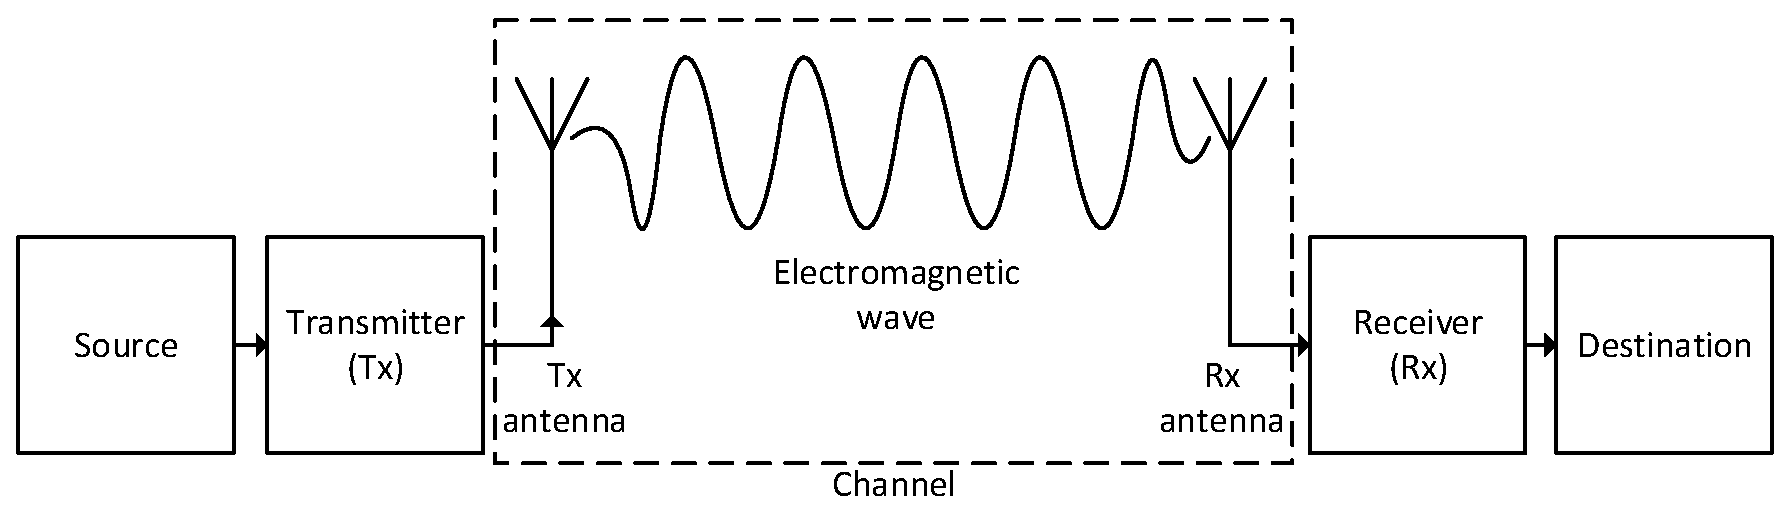
\includegraphics[width=\textwidth]{img/com_link.eps}
    \caption{Simple communication link.}
    \label{fig:com_link}
\end{figure}

\subsection{Mobile networks}
\label{sec:networks}

fsda fasdf df d \cref{sec:gsm,sec:3g,sec:lte}.

\subsubsection{Global System for Mobile communications}
\label{sec:gsm}
In 1982 the European Conference of Postal and Telecommunications Administrations (CEPT) founded the Groupe Spécial Mobile (GSM). Its purpose was to develop a new digital mobile communication system.  The new system had two requirements. First, it had to be efficient and technically better than previous wireless communication systems. It was clear at that time that analog systems would lack in user capacity, ease of use and number of additional services compared to digital system. Second, the previous analog systems were incompatible in different countries, so the new system should be standardized for whole Europe. \cite{molisch}

Developing GSM was a long process. Multiple proposals were developed by different companies. Proposals had covered nearly all possible technical solutions. Every proposed system was tested both in field and with a channel simulator. The decision was not made only based on technical aspects: also marketing and politics had influence. For example, for multiple access scheme, only Time Division Multiple Access (TDMA) was suitable. Signal processing needed for Code Division Multiple Access (CDMA) would have cost too much and was unreliable at the time. Frequency Division Multiple Access (FDMA) required antenna diversity at the mobile terminal. This would have been feasible but would have increased antenna sizes which was not desirable. However, the final developed TDMA system was a compromise. Reasons for this were political: standardizing one company's proposal would have given them a great competitive advantage. \cite{molisch}

First GSM systems were implemented in Europe after 1992. Soon it was realized that functionalities that originally had not been included in the standard were needed. These were developed by 1995. Later, General Packet Radio Service (GPRS) and the more efficient modulation of Enhanced Data rates for GSM Evolution (EDGE) have been included. \cite{molisch}
%%Lisää GPRS & EDGE data ratet vrt. alkuperäinen

GSM is the most successful mobile communication system worldwide. It had spread from Europe to all over the world, except Japan and Korea, where it was never implemented. Since GSM was now a worldwide standard, it was renamed Global System for Mobile communications. \cite{molisch}

GSM operates at three different carrier frequencies. Original systems use frequencies around 900\,MHz. Number of subscriptions increased which led to the addition of 1800\,MHz band. That band has more or less three times more bandwidth available than the original carrier. The new band also increased network capacity significantly. Third system operating at 1900\,MHz band is mainly used in the United States.  Table \ref{tab:gsm} below presents the key specifications and differences of the three versions of GSM. \cite{molisch}

\begin{table}[H]
    \centering
    \caption{Specifications of GSM carriers.} %lähde
    \label{tab:gsm}
    \begin{tabular}{|c|c|c|c|c|}
        \hline
         Carrier & Uplink frequency & Downlink frequency & Bandwith & Data rate \\%vai Capacity
         \hline
         GSM900 & 880-915\,MHz & 925-960\,MHz & & \\
         \hline
         GSM1800 & 1710-1785\,MHz & 1805-1880\,MHz & & \\
         \hline
         GSM1900 & 1850-1910\,MHZ & 1930-1990\,MHz & & \\
         \hline
    \end{tabular}
\end{table}

\subsubsection{Third generation mobile networks}
\label{sec:3g}
The success beyond expectations of GSM inspired the development of a new communication system. International Telecommunications Union (ITU) announced few goals for a standard called International Mobile Telecommunications (IMT-2000) for the third generation (3G) mobile communication system. The new system should have better performance, meaning better spectral efficiency and higher peak data rates: 2\,Mb/s indoor and 348\,kb/s outdoor. Same time, channel bandwidth should increase from 200\,kHz to 5\,MHz. Also new multimedia applications should be supported, which would require flexibility in choosing the data rates. Finally, the system should be backwards compatible with GSM. \cite{molisch}

In early 1990s, different European groups developed proposals for 3G within the European Telecommunications Standards Institute (ETSI). Proposed solutions ranged from TDMA and CDMA to new Orthogonal Frequency Division Multiplexing (OFDM). In 1998 two drafts were selected to form the European proposal for the new network standard: Wideband Code Division Multiple Access (WCDMA). First draft defined a Frequency Division Duplexing (FDD) mode which operates as the basic system. Second introduced a Time Division Duplexing (TDD) mode which supported high data rate applications. WCDMA usually refers to the radio access technology, and the complete 3G network is called Universal Mobile Telecommunication System (UMTS). \cite{molisch}

Europeans were not the only ones making proposals for the IMT-2000 family. Japanese also proposed a WCDMA system that was rather similar to the European, and thus merged. Besides the Europe-Japan collaboration, four other proposals had strong support, which made reaching an agreement for a single 3G system impossible within the ITU. As a compromise, ITU decided to declare all proposals as different modes of IMT-2000. Later Time Division Synchronous Code Division Multiple Access (TD-SCDMA) was an important part of 3G developments and then accepted to the IMT-2000 family. \cite{molisch}

The European/Japanese standard was further developed by the Third Generation Partnership Project (3GPP). Newer versions of the standard included improvements, such as High-Speed Packet Access (HSPA). It was first implemented for downlink and later realized for uplink also. Different UMTS technologies are compared in the table \ref{tab:3g} below. \cite{molisch} %%Täytä taulukko WCDMA vs TD-SCDMA vs HSPA %%kerro tekstissä taajuudet jne teknistä dadaa.

\begin{table}[H]
    \centering
    \caption{Comparison of different 3G technologies.} %lähteet
    \label{tab:3g}
    \begin{tabular}{|c|c|c|c|}
         \hline
         Standard &  Frequencies & Bandwidth & Peak data rate\\
         \hline
         WCDMA & & &\\
         \hline
         TD-SCDMA & & &\\
         \hline
         HSPA & & &\\
         \hline
    \end{tabular}
\end{table}

The number of different specifications had grown so much that it was a problem for 3GPP. Increased costs and delays in time to market nearly killed 3G. First UMTS networks were planned to start operating in 2002, but it took off only around 2005. Besides technical problems also lack of applications requiring high data rates in the market delayed the implementation. By 2009 these problems were solved and UMTS had become successful all around the world. \cite{molisch}

\subsubsection{Long-Term Evolution}
\label{sec:lte}
While WCDMA was being deployed and spreading out, 3GPP started to research a new, fourth generation (4G) network system. They supposed that data rates and spectral efficiencies of WCDMA would not be sufficient for the future applications and demands. The new standard was named Long-Term Evolution (LTE) and it was constructed from a scratch and differences to previous standards were significant. LTE uses Orthogonal Frequency Division Multiple Access (OFDMA) scheme, OFDM modulation and has a limited support for Multiple Input Multiple Output system (MIMO) antenna technology. Also its core network is purely packet-switched while GSM was circuit-switched and 3G a combination of the two. \cite{molisch}

For 4G network standard, IMT-Advanced, ITU announced requirements in 2008. Such systems should provide access to advanced mobile services and have capabilities for high quality multimedia applications. The performance requirements included better spectral efficiency, scalable bandwidth up to at least 40\,MHz and peak data rates of 1\,Gb/s. \cite{itur} However, LTE has peak data rate of 300\,Mb/s, which is not fulfilling the IMT-Advanced standard. Further development have extended the use of MIMO for better spectral efficiency. Newer release called LTE-Advanced is promising 1\,Gb/s peak data rates and is one candidate for IMT-Advanced cellular system. \cite{molisch} %%viittaus taulukkoon alla, täytä taulukko

\begin{table}[H]
    \centering
    \caption{LTE and LTE-Advanced fulfillment of IMT-Advanced \cite{parkvall_lte}.}
    \label{tab:lte}
    \begin{tabular}{|l|M{3cm}|M{3cm}|M{3cm}|}
        \hline
         & IMT-Advanced requirement & LTE & LTE-Advanced \\
        \hline
        Peak data rate & & & \\
        -Downlink & & & \\
        -Uplink  &  & & \\
        \hline
        Spectral efficiency & & & \\
        -Downlink & 15\,b/s/Hz & 16\, b/s/Hz & 16\, b/s/Hz*\\
        -Uplink  & 6.75\, b/s/Hz & 4\, b/s/Hz & 8.1\, b/s/Hz**\\
        \hline
        Bandwidth & At least 40\,MHz & Up to 20\,MHz & Up to 100\,MHz \\
        \hline
    \end{tabular}
    
    *For 4x4 MIMO antenna system. 8x8 could reach 30\,b/s/Hz.\\
    **For 2x2 MIMO antenna system. 4x4 could reach 16.1\,b/s/Hz.
\end{table}

4G systems should be backwards compatible with 3G and GSM. Also the transitions from older technology to newer one should be smooth, which requires two system to coexist and use the same frequency bands. LTE and LTE-Advanced operate on a number frequency bands. Due to the national frequency regulators, all bands are not available in all countries. Since some frequencies are already allocated to e.g.\ WCDMA or GSM, corresponding frequency bands are created and operators are anticipated to migrate. All frequency bands are listed in table \ref{tab:lte_bands} below. \cite{molisch, radio_electronics}

\begin{table}[H]
    \centering
    \caption{LTE frequency band allocation for FDD and TDD modes. \cite{radio_electronics}}
    \label{tab:lte_bands}
    \begin{tabular}{|c|c|c|}
        \hline
        \multicolumn{3}{|c|}{FDD bands} \\
        \hline
         Band & Uplink (MHz) & Downlink (MHz) \\
         \hline
         1 & 1920 - 1980 & 2110 - 2170\\
         \hline
         2 & 1850 - 1910 & 1930 - 1990\\
         \hline
         3 & 1710 - 1785 & 1805 - 1880\\
         \hline
         4 & 1710 - 1755 & 2110 - 2155\\
         \hline
         5 & 824 - 849 & 869 - 894\\
         \hline
         6 & 830 - 840 & 875 - 885\\
         \hline
         7 & 2500 - 2570 & 2620 - 2690\\
         \hline
         8 & 880 - 915 & 925 - 960\\
         \hline
         9 & 1749.9 - 1784.9 & 1844.9 - 1879.9\\
         \hline
         10 & 1710 - 1770 & 2110 - 2170\\
         \hline
         11 & 1427.9 - 1452.9 & 1475.9 - 1500.9\\
         \hline
         12 & 698 - 716 & 728 - 746\\
         \hline
         13 & 777 - 787 & 746 - 756\\
         \hline
         14 & 788 - 798 & 758 - 768\\
         \hline
         15 & 1900 - 1920 & 2600 - 2620\\
         \hline
         16 & 2010 - 2025 & 2585 - 2600\\
         \hline
         17 & 704 - 716 & 734 - 746\\
         \hline
         18 & 815 - 830 & 860 - 875\\
         \hline
         19 & 830 - 862 & 791 - 821\\
         \hline
         20 & 832 - 862 & 791 - 821\\
         \hline
         21 & 1447.9 - 1462.9 & 1495.5 - 1510.9\\
         \hline
         22 &  3410 - 3500 & 3510 - 3600\\
         \hline
         23 & 2000 - 2020 & 2180 - 2200 \\
         \hline
         24 & 1625.5 - 1660.5 & 1525 - 1559\\
         \hline
         25 & 1850 - 1915 & 1930 - 1995\\
         \hline
         26 & 814 - 849 & 859 - 894\\
         \hline
         27 & 807 - 824 & 852 - 869\\
         \hline
         28 & 703 - 748 & 758 - 803\\
         \hline
         29 & downlink only & 717 - 728 \\
         \hline
         30 & 2305 - 2315 & 2350 - 2360\\
         \hline
         31 & 452.5 - 457.5 & 462.5 - 467.5\\
         \hline
         \hline
         \multicolumn{3}{|c|}{TDD bands} \\
         \hline
         Band & \multicolumn{2}{|c|}{Allocation (MHz)}\\
         \hline
         33 & \multicolumn{2}{|c|}{1900 - 1920}\\
         \hline
         34 & \multicolumn{2}{|c|}{2010 - 2015}\\
         \hline
         35 & \multicolumn{2}{|c|}{1850 - 1910 }\\
         \hline
         36 & \multicolumn{2}{|c|}{1930 - 1990 }\\
         \hline
         37 & \multicolumn{2}{|c|}{1910 - 1930 }\\
         \hline
         38 & \multicolumn{2}{|c|}{2570 - 2620}\\
         \hline
         39 & \multicolumn{2}{|c|}{1880 - 1920 }\\
         \hline
         40 & \multicolumn{2}{|c|}{2300 - 2400}\\
         \hline
         41 & \multicolumn{2}{|c|}{2496 - 2690 }\\
         \hline
         42 & \multicolumn{2}{|c|}{3400 - 3600 }\\
         \hline
         43 & \multicolumn{2}{|c|}{3600 - 3800}\\
         \hline
         44 & \multicolumn{2}{|c|}{703 - 803}\\
         \hline
    \end{tabular}
\end{table}

\clearpage


\section{Mobile antennas}
\label{sec:mobile_antennas}

\subsection{Antennas in general}
\label{sec:general_antennas}
An antenna is the single most important part of a radio system. The purpose of an antenna is to transmit and receive radio waves. Thus, it is designed to transform guided electromagnetic waves to free space waves, and vice versa \cite{holopainen_phd}. As an electrical signal travels from one point to another via transmission line, e.g.\ coaxial cable or waveguide, the carried energy is bounded to the line or very nearby. Comparably, antennas work the other way: they are encouraging signals to propagate as far away from the antenna as possible, i.e.\ to radiate \cite{stutzman}.

\begin{figure}[H]
    \centering
    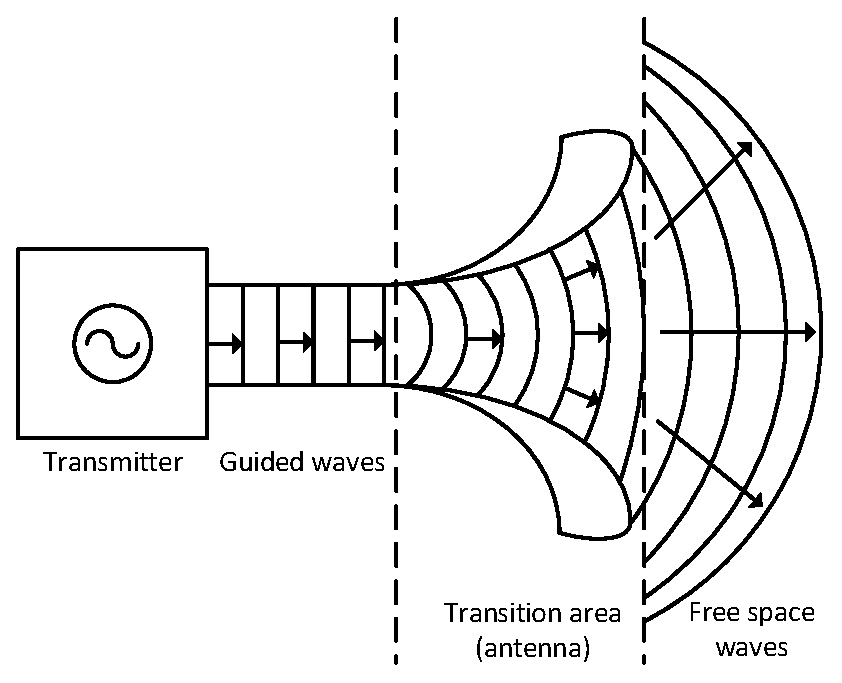
\includegraphics[width=0.7\textwidth]{img/antenna_principle.eps}
    \caption{Principle of antenna operating in transmission presented in \cite{saunders}.}
    \label{fig:antenna_principle}
\end{figure}

%how antennas radiate
Antennas radiate because of accelerated charges \cite{stutzman}. Acceleration causes disturbance that initiates electromagnetic fields to propagate away from the source of disturbance. The acceleration of charges occurs as change of speed or direction of the charge. As an example, a case of a single thin wire and single charge can be considered. Figure \ref{fig:charges} illustrates the following situations \cite{saunders, balanis}:
\begin{enumerate}
    \item Stationary charge will not create radiation, since there is no current (\ref{fig:no_move}).
    \item Charge moving with constant speed will not create radiation, if the wire is straight and infinitely long (\ref{fig:infinite}).
    \item Charge moving with constant speed creates radiation, if the wire is either curved (\ref{fig:curved}), bent (\ref{fig:bent}), discontinuous (\ref{fig:discont}), terminated (\ref{fig:terminated}) or truncated (\ref{fig:truncated}).
    \item Charge oscillating periodic motion creates radiation (\ref{fig:osc}).
\end{enumerate}

\begin{figure}[H]
    \centering
    \begin{subfigure}[b]{0.4\textwidth}
        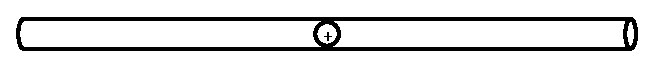
\includegraphics[width=\textwidth]{img/radiations_no_movement.eps}
        \caption{No radiation.}
        \label{fig:no_move}
    \end{subfigure}
    \begin{subfigure}[b]{0.4\textwidth}
        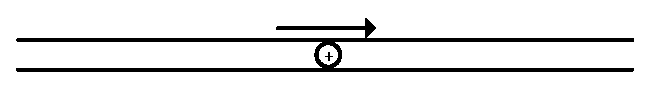
\includegraphics[width=\textwidth]{img/radiations_infinite.eps}
        \caption{No radiation.}
        \label{fig:infinite}
    \end{subfigure}
    
    \begin{subfigure}[b]{0.4\textwidth}
        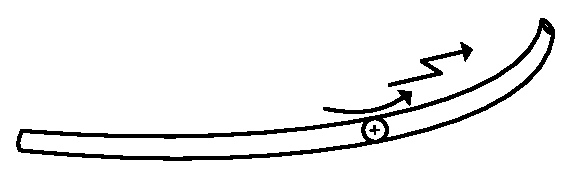
\includegraphics[width=\textwidth]{img/radiations_curved.eps}
        \caption{Radiates.}
        \label{fig:curved}
    \end{subfigure}
    \begin{subfigure}[b]{0.4\textwidth}
        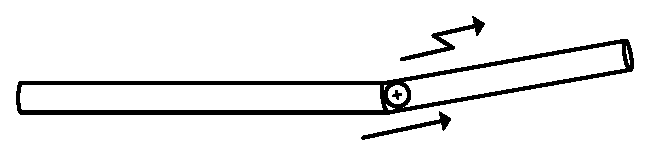
\includegraphics[width=\textwidth]{img/radiations_bent.eps}
        \caption{Radiates.}
        \label{fig:bent}
    \end{subfigure}
    
     \begin{subfigure}[b]{0.4\textwidth}
        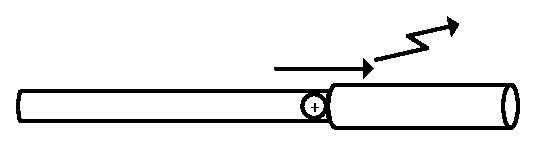
\includegraphics[width=\textwidth]{img/radiations_discont.eps}
        \caption{Radiates.}
        \label{fig:discont}
    \end{subfigure}
    \begin{subfigure}[b]{0.4\textwidth}
        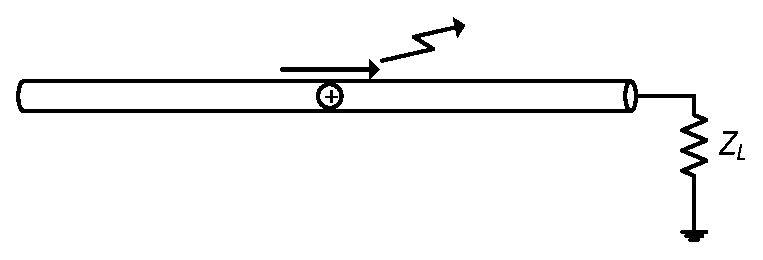
\includegraphics[width=\textwidth]{img/radiations_terminated.eps}
        \caption{Radiates.}
        \label{fig:terminated}
    \end{subfigure}
    
     \begin{subfigure}[b]{0.4\textwidth}
        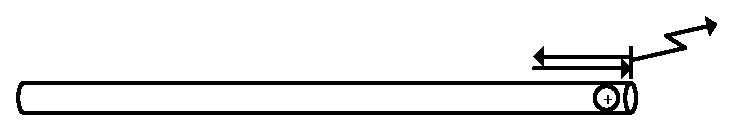
\includegraphics[width=\textwidth]{img/radiations_truncated.eps}
        \caption{Radiates.}
        \label{fig:truncated}
    \end{subfigure}
    \begin{subfigure}[b]{0.4\textwidth}
        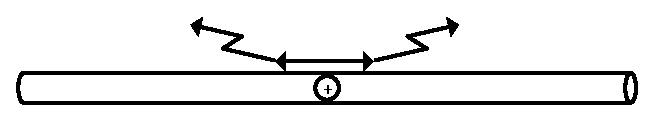
\includegraphics[width=\textwidth]{img/radiations_osc.eps}
        \caption{Radiates.}
        \label{fig:osc}
    \end{subfigure}
    
    \caption{Examples of charges producing radiation. Re-illustrated from \cite{saunders, balanis}.}
    \label{fig:charges}
\end{figure}

These described situations are the most elementary examples of radiation. In real world the normal case is steady-state charge oscillating, usually sinusoidally, and the oscillation frequency equals to the radiation frequency \cite{stutzman}. Once accelerated charges have started a wave, they are not needed anymore. Wave can sustain itself by closing electric field lines on themselves, since there are no charges present. %\cite{stutzman}

Maxwell discovered that fields surrounding a transmission line, are guided by the line itself \cite{stutzman}. In open-ended transmission line a standing wave is formed by the interaction between the incident wave and reflections. The standing wave has zero current at the end of the line and nulls every half wave length from there. The current flowing in transmission line wire are headed in opposite directions, which creates strong, constructive interference of electric and magnetic fields between the wires. Bending quarter-wave long parts from the ends of both wires outwards exposes the reinforced fields to open space. In the formed half-wavelength dipole antenna the currents are flowing to the same direction and the maximum of its current distribution lies in between the halves \cite{stutzman}. Thus, antenna is a structure that radiates. %\cite{stutzman}

%when used
Radiated waves propagate away from the antenna, to all directions, although not uniformly as antennas do not have any guiding structures in contrast to transmission lines \cite{stutzman}. Antennas are usually rather used than transmission lines when either the operating frequency is high or distance between transmitter and receiver is large. Increment of either of those increases costs and signal losses of transmission lines, which often makes antennas and wireless transmission preferable choice. %\cite{stutzman}


\subsection{Small antennas}
\label{sec:small_antennas}
Mobile antennas are typical examples of small antennas. Small antennas can be defined a few different ways \cite{modern_small_antennas}. \emph{Electrically small antennas (ESA)} are not necessarily small in size, but they are small compared to wavelength. An ESA can be surrounded with a sphere of radius $r\leq\frac{\lambda_0}{2\pi}$, where $\lambda_0$ is the free space wavelength at operating frequency. An antenna can also be \emph{physically small (PSA)} if its measured dimensions are small. PSAs do not have any exact definition, rather than a sensual view of smallness. For this thesis, the main focus is on electrically small antennas.

As it was mentioned previously in section \ref{sec:general_antennas}, antennas radiate on a certain frequency, called resonance frequency ($f_0$). The wavelength $\lambda_0$ is related to the frequency via propagation speed, which in free space is the speed of light $c$ \cite{stutzman}:
\begin{equation}
\label{eq:fcl}
    f_0 = \frac{c}{\lambda_0}.
\end{equation}
At resonance, a standing wave is formed at the antenna \cite{stutzman}. Since the resonance frequency is the same as the radiation frequency, the size of an antenna is related to the wavelength. For an electrically small antenna, the physical size of it is only a fraction of wavelength. Small electrical size results in small input resistance and large capacitive (or inductive for some antenna types) input reactance \cite{modern_small_antennas}. The input impedance of an antenna at resonance is (almost) purely resistive, and outside that frequency the impedance of an ESA is changing quickly and therefore being the main limiting factor for usable bandwidth \cite{holopainen_phd}. This characteristics makes wide band matching and thus achieving wide band performance difficult for electrically small antennas.

The three important characteristics of an electrically small mobile antenna are size, efficiency, and bandwidth, which are all interconnected \cite{holopainen_phd}. Wider bandwidth could be achieved with larger antenna, which is not desirable in a modern mobile phone. Decreasing efficiency might increase bandwidth, but it would also decrease handset's battery life. Thus, improving one of these parameters is possible by worsening the others. The important challenge in small antenna design is to find a good trade-off between the three parameters for each application.

\subsubsection{Requirements for mobile antennas}
\label{sec:requirements}
Antennas used in handsets and other handheld devices operate in demanding environment. Orientation of the phone is rather random, especially in standby mode. Signal between terminal and base station propagates in every way from line-of-sight to wide multipath arrival angles. Signal strength has to be adequate to counter fading from human head and hand. Hand-effect is a major problem for mobile antennas. Studies have shown that up $70\,\%$ of the radiated power might get absorbed into user's hands \cite{valkonen_phd}. Generally, the requirements for mobile antennas can be listed in the following way \cite{saunders, lehtovuori_phd}:
\begin{enumerate}
    \item \textit{Radiation pattern:} Due to the randomly changing orientation of the phone, omnidirectional pattern in azimuth is desirable, as well as wide beamwidth vertically. Though, the precise pattern is not that important given the propagation environment and the proximity of the user.
    \item \textit{Input impedance:} Considering the number of used frequency bands today, phones have wide operational bandwidths. Antenna should be well matched to the source at all required bands.
    \item \textit{Efficiency:} Since omnidirectional antennas have low gain, it is critical to have good efficiency in order to transform input power to radiation. Efficiency might be the most important figure-of-merit for mobile antennas.
    \item \textit{Size:} Mobile devices consist of many subsystems, and nowadays require multiple antennas. Together with the constrained physical size of the handset, the antennas should be as small as possible. However, small size creates challenges as other requirements cannot be neglected.
    \item \textit{Manufacturability:} Mobile phone antenna is useless if it is not robust against mechanical damages or cannot be mass produced with reasonable costs. Also, antennas should fit the appearance requirements of the consumer product. 
\end{enumerate}

The following \cref{sec:efficiency,sec:matching,sec:pattern,sec:bandwidth} explain the first three of these requirements in more detail.

\subsection{Antenna impedance \& efficiency}
\label{sec:efficiency}
An antenna can be modeled with an electrical equivalent circuit consisting of two resistances and one reactance (Figure \ref{fig:antenna_equivalent}) \cite{stutzman,balanis,saunders}. One of the resistances represents ohmic and other losses ($R_o$) and the other is radiation resistance, $R_r$. It models the power loss from the circuit due to radiation, i.e.\ radiated power. Antenna's input impedance is defined as \cite{stutzman, balanis}:
\begin{equation}
\label{eq:input_impedance}
    Z_a=R_a+\j X_a
\end{equation}
where antenna resistance $R_a=R_o+R_r$ and $X_a$ is antenna reactance, which models the energy stored in the near-field of the antenna. %\cite{stutzman}

\begin{figure}[H]
    \centering
    \begin{circuitikz}[wave/.style={decorate,decoration={snake,post length=1.4mm,amplitude=2mm,segment length=2mm},thick}]
        \draw 
            (0,0) to[sI] (0,2)
            (0,2) to[R, l_=$R_s$] (2,2)
            (2,2) to[european resistor, l_=$X_s$] (4,2)
            (6,2) to[R, l^=$R_r$] (6,0)
            (0,0) to[short] (4,0);
        \draw [densely dashed] (4,2.7) to[short] (4,-0.7);
        \draw 
            (4,2) to[R, o-, l_=$R_o$] (6,2)
            (4,0) to[european resistor, o-, l^=$X_a$, n=res] (6,0)
            (5,-0.3) node[label={below:Antenna}]{}
            (2,-0.3) node[label={below:Transmitter}]{};
        \draw [->,wave] (6.7,1.7)--(7.7,2) node[]{};
        \draw [->,wave] (6.7,0.3)--(7.7,0) node[]{};
    \end{circuitikz}
    \caption{Equivalent circuit for a generator connected to an antenna. \cite{saunders}}
    \label{fig:antenna_equivalent}
\end{figure}

In the electrical equivalent circuit, the antenna is connected to a generator. Some of the input power $\sub{P}{in}$ is dissipated in ohmic losses, and only a portion of it, $\sub{P}{rad}$ is radiated. Radiation efficiency describes how much of the power is radiated, in other words utilized. The radiation efficiency is given as \cite{pozar}:

\begin{equation}
\label{eq:efficiency}
    \sub{\eta}{rad} = \frac{\sub{P}{rad}}{\sub{P}{in}} = \frac{R_r}{R_r+R_o}.
\end{equation}

Efficiency can also be approximated with system's $S$-parameters. As radiated power is considered as power lost from system, all $S$-parameters of an $N$-port system are required when determining the radiated power. For lossless system, efficiency for port $i$ can be expressed as \cite{lehtovuori_phd}:
\begin{equation}
\label{eq:eff_aprx}
    \sub{\eta}{rad} = 1-\sum_{j=1}^{N}|S_{ij}|^2
\end{equation}
where $S_{ij}$ are the scattering parameters expressing the power flow from port $j$ to port $i$. For other than lossless systems this works only as an approximation due to e.g. substrate or ohmic losses \cite{lehtovuori_phd}.

Good efficiency may be the most important property for any antenna. In transmission, that means a smaller transmit power is needed for the wanted field strength. In reception, a higher SNR can be achieved as it is proportional to efficiency. Therefore, an efficient antenna can improve link quality and battery life of handset \cite{molisch}. In an ideal situation, $\sub{\eta}{rad}=1$. As mobile antennas operate on wide range of frequencies, this is impossible to realize. %\cite{molisch}


\subsection{Radiation characteristics}
\label{sec:pattern}
Radiation pattern shows the far-field radiation properties of an antenna \cite{balanis, stutzman}. It tells the strength and phase of radiation in certain direction with respect to an isotropic radiator of same energy \cite{balanis}. Isotropic radiator is physically unrealizable, but it is used as reference of radiation charactics due its definition: lossless antenna radiating equally to all directions \cite{balanis}. More realistic type is directional antenna \cite{balanis}, which radiates significantly more efficiently in some direction than in others. Special type of this pattern is referred as omnidirectional \cite{balanis}, which has nondirectional pattern in a given plane (usually azimuth plane) and directional in an orthogonal plane (usually elevation plane).

Usually the pattern is expressed as a function of the directional coordinates: azimuth angle $\phi$ and elevation angle $\theta$. Strengths of radiated electric or magnetic fields in the far-field are referred to field patterns, while the power density of them is power pattern. Often radiation patterns are normalized to their maximum values \cite{stutzman}:
\begin{equation}
\label{eq:f_norm}
    F(\theta,\phi)=\frac{E_\theta}{E_\theta(\mathrm{max})}
\end{equation}
where $E_\theta$ is the $\theta$-component of the electrical field and $E_\theta(\mathrm{max})$ is its maximum value. For any radiating element, field patterns can be expressed in a general form \cite{stutzman}:
\begin{equation}
\label{eq:f_gen}
    F(\theta,\phi) = g(\theta,\phi)f(\theta,\phi)
\end{equation}
where $g(\theta,\phi)$ and $f(\theta,\phi)$ are element and pattern factors, respectively. Pattern factor is an integral over the current distribution in space and element factor is the pattern of an infinitesimal current in the distribution \cite{stutzman}.

Generally, for a good communications link, it is useful to know how an antenna concentrates the radiated energy. Directivity describes this property. Normally, the word \textit{directivity} refers to the maximum directivity ($\sub{D}{max}$) of an antenna, but the parameter is actually dependent of the observation point. It is defined as the ratio of radiation intensity in a direction to the average intensity. Directivity in a certain direction can be expressed with normalized power pattern \cite{stutzman}:
\begin{equation}
\label{eq:dir}
    D(\theta, \phi) = \sub{D}{max}|F(\theta,\phi)|^2.
\end{equation}

Thus, directivity is purely directional characteristic determined by the power pattern of an antenna. As antennas are parts of a radio system, besides their ability to focus radiation to certain direction, also their capabilities of transforming power at input terminals to radiation is practical to know. The feature combining all this information is called antenna's gain. Since all of the input power is not radiated, and especially electrically small antennas are very inefficient, gain might be more useful than directivity in case of mobile antennas. Gain is defined as \cite{stutzman}:
\begin{equation}
    \label{eq:gain}
    G(\theta,\phi) = \sub{\eta}{rad}D(\theta,\phi).
\end{equation}

Mobile antennas typically have more or less omnidirectional pattern \cite{ying_mobile_antennas}, due to the fact, that user cannot know where the nearest base station is. Since omnidirectional pattern is nondirectional in one plane, antennas of that type usually have low gain which makes efficiency even more important parameter for mobile antennas.

\subsection{Impedance matching}
\label{sec:matching}
As the primary objective of an antenna is to convert waves bounded to transmission line to free space waves, antenna has to be matched to the source in order to avoid reflections. Matching also improves Signal-to-Noise Ratio (SNR) of the system and reduces amplitude and phase errors \cite{pozar}. Reflections occur in the connection point of transmission line and antenna, and large reflections prevent maximizing radiated power in transmission or utilized power in receiving. Maximum power is obtained when antenna is conjugate matched to the source impedance $Z_s=R_s+\j X_s$ (or to load impedance, respectively) \cite{stutzman}:
\begin{align}
\label{eq:matching1}
    Z_s^* &= Z_a\\
\label{eq:matching2}
    R_s-\j X_s &= R_a+\j X_a.
\end{align}
For perfectly matched antenna, reflection coefficient is zero. Reflection coefficient $\Gamma$ is defined followingly \cite{stutzman}: 
\begin{equation}
\label{eq:reflection_coeff}
    \Gamma = \frac{Z_a-Z_s^*}{Z_a+Z_s}.
\end{equation}

In an ideal situation, perfect matching can be obtained at a single frequency. This is stated by Bode-Fano criterion for different load topologies. For parallel $RC$-load, the criterion is given as \cite{pozar}:
\begin{equation}
    \int_0^\infty\ln\frac{1}{|\Gamma(f)|}df\leq\frac{\pi}{RC}
\end{equation}
where $\Gamma(f)$ is the reflection coefficient as a function of frequency and $R$ and $C$ are the resistance and capacitance of the load, respectively. The criterion describes an upper limit of performance. Further analysis on this, which is out of the scope of this thesis, results few conclusions \cite{pozar}:
\begin{itemize}
    \item broader bandwidth can be achieved only if reflection coefficient increases.
    \item reflection coefficient can reach 0 only at discrete frequencies, i.e. having bandwidth of 0.
    \item if load impedance increases, matching level decreases. Therefore circuits with higher quality factor ($Q$) are harder to match than low-$Q$ circuits.
\end{itemize}

Matching can be achieved in several different ways, as presented in \cite{pozar}, and probably the simplest possible is \textit{L-section} matching network of two lumped elements. Figure \ref{fig:l-match} shows the two possible layouts for L-section. In both configurations, the reactive elements can have any inductor-capacitor combination, in order to match the antenna. The exact matching circuit depends on the antenna impedance. With low frequencies, up to about 2\,GHz \cite{holopainen_phd}, or small circuit size, L-section matching is feasible. Limitations of L-section come in the way when frequency or circuit size increases.

\begin{figure}[h]
    \centering
    \begin{subfigure}[b]{0.4\textwidth}
        \begin{circuitikz}
            \draw
                (0,0) to[short, o-] (1,0)
                (1,0) to[european resistor, l_=$\j X$] (3,0)
                (3,0) to[european resistor, l_=$\j B$] (3,-2)
                (3,0) to[short, -o] (4,0)
                (4,0) to[short] (5,0)
                (5,0) to[european resistor, l^=$Z_a$] (5,-2)
                (0,-2) to[short, o-o] (4,-2)
                (4,-2) to[short] (5,-2);
        \end{circuitikz}
        \caption{Parallel susceptance first.}
        \label{fig:l-match1}
    \end{subfigure}
    \begin{subfigure}[b]{0.4\textwidth}
        \begin{circuitikz}
            \draw
                (0,0) to[short, o-] (1.5,0)
                (1.5,0) to[european resistor, l_=$\j B$] (1.5,-2)
                (1.5,0) to[european resistor, l_=$\j X$] (3.5,0)
                (3.5,0) to[short, -o] (4,0)
                (4,0) to[short] (5,0)
                (5,0) to[european resistor, l^=$Z_a$] (5,-2)
                (0,-2) to[short, o-o] (4,-2)
                (4,-2) to[short] (5,-2);
        \end{circuitikz}
        \caption{Series reactance first.}
        \label{fig:l-match2}
    \end{subfigure}
    \caption{The two layouts for L-section matching circuit \cite{pozar}. Elements are either capacitors or inductors.}
    \label{fig:l-match}
\end{figure}

Usually applications, such as mobile antennas, require wider band of frequencies. Although perfect wideband matching is impossible, antennas can be wideband matched to an adequate level, but it probably increases complexity of the system \cite{pozar}. Clearly, complexity is an undesired matter, since simpler matching solutions are usually smaller, cheaper and more reliable. In case of wideband matching, matching network might have to be adjustable in order to operate properly in the whole band. Figure \ref{fig:3elem_match} shows examples of different topologies of three elements, that are used with mobile antennas \cite{lehtovuori_cce_bw}.

\begin{figure}[H]
    \centering
    \begin{subfigure}[b]{0.4\textwidth}
        \begin{circuitikz}
            \draw
                (0,0) to[short, o-] (2,0)
                (2,0) to[european resistor] (2,-2)
                (2,0) to[european resistor] (4,0)
                (4,0) to[european resistor] (4,-2)
                (4,0) to[short] (5,0)
                (5,0) to[european resistor, l^=$Z_a$] (5,-2)
                (0,-2) node[]{}
                (0,-2) to[short,o-] (5,-2);
        \end{circuitikz}
        \caption{$\Pi$-topology}
        \label{fig:p-match}
    \end{subfigure}
    \begin{subfigure}[b]{0.4\textwidth}
        \begin{circuitikz}
            \draw
                (0,0) to[european resistor, o-] (2,0)
                (2,0) to[european resistor] (4,0)
                (2,0) to[european resistor] (2,-2)
                (4,0) to[short] (5,0)
                (5,0) to[european resistor, l^=$Z_a$] (5,-2)
                (0,-2) node[]{}
                (0,-2) to[short,o-] (5,-2);
        \end{circuitikz}
        \caption{T-topology.}
        \label{fig:t-match}
    \end{subfigure}
    
    \begin{subfigure}[b]{0.4\textwidth}
        \begin{circuitikz}
            \draw
                (0,0) to[short, o-] (2.5,0)
                (1,0) to[L] (1,-2)
                (2,0) to[C] (2,-2)
                (2.5,0) to[european resistor] (4.5,0)
                (4.5,0) to[short] (5,0)
                (5,0) to[european resistor, l^=$Z_a$] (5,-2)
                (0,-2) node[]{}
                (0,-2) to[short,o-] (5,-2);
        \end{circuitikz}
        \caption{F-topology.}
        \label{fig:f-match}
    \end{subfigure}
    \begin{subfigure}[b]{0.4\textwidth}
        \begin{circuitikz}
            \draw
                (0,0) to[C, o-] (2,0)
                (2,0) to[L] (4,0)
                (4,0) to[european resistor] (4,-2)
                (4,0) to[short] (5,0)
                (5,0) to[european resistor, l^=$Z_a$] (5,-2)
                (0,-2) node[]{}
                (0,-2) to[short,o-] (5,-2);
        \end{circuitikz}
        \caption{$\Gamma$-topology.}
        \label{fig:g-match}
    \end{subfigure}
    \caption{Four different matching networks consisting of three lumped elements. Blocks can be either capacitors or inductors \cite{lehtovuori_cce_bw}.}
    \label{fig:3elem_match}
\end{figure}


Besides matching with reactive elements, also transmission line stubs can be used \cite{pozar}. Stub can be either shorted or open-ended, and in parallel or in series with the feed line. One advantage of \textit{single-stub tuning} is that it can be manufactured along with transmission line media. Parallel stubs are useful with microstrip lines and series stubs with coplanar waveguides or slotlines.

While matching with a single stub, the matching level depends on distance from the antenna and the length of the stub. By choosing the length of the stub correctly, any reactance or susceptance can be obtained. %\cite{pozar}

A major disadvantage with single-stub tuning is the distance between antenna and stub, especially when adjustable matching is desired. When matching for a single frequency, this should not be a problem. However, using a \textit{double-stub tuner} might help with tunable matching solution. It has two stubs at fixed locations, which makes the distance between the stubs and from the antenna constants. The first stub may even be connected directly to the antenna. Although, double-stub tuner is not able to match all antenna impedances. %\cite{pozar}


\subsection{Bandwidth}
\label{sec:bandwidth}
Bandwidth expresses the operational frequency range of an antenna \cite{balanis}. Bandwidth can be described as percentage from a center frequency (e.g.\ resonance frequency of a dipole) or range from lower to upper limit (broadband antennas), where different parameters (e.g.\ gain, efficiency, matching) are still at acceptable level. Since antenna characteristics vary from not-at-all frequency dependent to critically affected by frequency, bandwidth cannot be clearly characterized. Usually it is specified for each application.

Bandwidth can be divided to pattern and impedance bandwidths \cite{balanis}. Pattern bandwidth is associated with gain, side lobe level, and beamwidth while impedance bandwidth relates to input impedance, matching, and radiation efficiency.

Mobile terminals require wide operational bandwidth, and small antennas are typically providing narrow bandwidth. As explained in the previous sections, there is a contradiction between these two requirements, which can be solved by finding a good trade-off between them. Bandwidth can be increased at the expense of antenna size or efficiency, and fortunately, some methods provide more benefits than damage \cite{holopainen_phd}. Multi-resonant matching circuits provide an efficient way to improve bandwidth. Adding resonators can double or triple the available bandwidth, but at the same time the complexity and losses of the whole system increase. Besides multiple resonators, wider bandwidth can be achieved with frequency tunable matching circuits. If the operational band can be split into sub-bands, that are not simultaneously used, digitally tunable capacitors (DTC) can be used. As well as with multi-resonators, using DTCs also increase complexity and losses in the system. Example of a matching circuit with DTC is used in \cite{ilvonen_pier} and shown in Figure \ref{fig:dtc_match}. Third way to increase bandwidth is to sacrifice efficiency. Accepting worse matching level might nearly double the bandwidth \cite{holopainen_phd}, and efficiency would weaken mainly at the borders of the frequency band.


\begin{figure}[H]
\centering
\begin{circuitikz}
    \draw (-1,0) node[label={above:feed}] {};
    \draw (-1,0) to[short, o-] (0,0);
    \draw (0,0) to[L, l^=$L_2$] (2,0);
    \draw (2,0) to[C, l^=$C_1$] (4,0);
    \draw (4,-2) to[vC, l^=DTC] (4,0);
    \draw (4,-2) node[ground]{};
    \draw (4,0) to[short] (6,0);
    \draw (6,0) to[L, l_=$L_1$] (6,-2);
    \draw (6,-2) node[ground]{};
    \draw (6,0) to[short] (8,0);
    \draw (8,0) to[short] (8.5,0.5);
    \draw (8,0) to[short] (8.5,-0.5);
\end{circuitikz}
    \caption{Example of a matching network of three lumped elements and a DTC presented in \cite{ilvonen_pier}.}
    \label{fig:dtc_match}
\end{figure}

\subsection{Typical antenna structures in mobile phones}
\label{sec:antenna_types}

\subsubsection{Dipoles and monopoles}
\label{sec:dipole}

Probably the most fundamental antenna type is dipole, which by the simplest is a transmission line with both wires bent at one end \cite{stutzman}. Dipole is often used as an example of an antenna especially in educational purposes due to its simple structure. As dipoles are resonating antennas, their operational frequency depends on their length. The most widely used one is half-wave long dipole.  By nature, dipoles are narrow band antennas, but wider bandwidth can be achieved e.g.\ by using larger wire width \cite{stutzman,balanis}. However, even if dipoles are electrically small, they are usually physically large structures, which is not favorable for mobile and handheld devices. Nevertheless, dipoles have also good features, like high efficiency and omnidirectional radiation pattern, that are wanted from mobile antennas.

Besides dipoles being physically too large for mobile applications, mobile antennas are surrounded by very nearby objects, that are harmful to the antenna. Normally, these objects are ground planes that are large compared to the antenna. Conductive ground planes affect antenna's performance, especially impedance and radiation pattern \cite{stutzman}. However, monopole antennas are designed to operate in the presence of a ground plane. Monopole is basically a dipole cut in half, and fed against a ground plane \cite{stutzman}. Monopole's impedance is half of dipole's, and hence, the radiated power is also half. This yields lower average radiation intensity which gives higher directivity. Operational frequency of a monopole of course depends on the length of the antenna, similarly to dipoles, but their smaller size makes monopoles more suitable for mobile devices.

\subsubsection{Microstrip antennas}
\label{sec:microstrip}

Microstrip antennas (MSA) are an alternative to wire antennas. For example, dipoles can be printed as microstrip lines. Typical microstrip antenna has a printed patch on top of a substrate with a ground plane below it \cite{stutzman}. MSAs are very low profile, since substrate is thin and the patch itself normally has thickness of $0.05\lambda_0$ or less. One advantage of microstrip antennas is that they can be included in microwave integrated circuits, which decreases costs, and provides controlled-dimension construction. Patches can also be printed on flexible substrates, which enables better use of available space \cite{stutzman}.

Microstrips radiate with broad beam broadside to the patch as the ground plane prevents the formation of back lobes. Challenges of patch antennas are that they are resonant antennas, which leads to narrow bandwidth. Also after fabrication, antenna cannot be re-adjusted easily. Due to the narrowband nature of this antenna type, and possibly large size, it is not very popular antenna for cellular phones \cite{stutzman}. However, Global Positioning System (GPS) is a standard feature in new mobile phones and it operates on a narrow band, and thus, microstrips with large dielectric constant substrate to reduce size are used for that purpose \cite{stutzman}.

\subsubsection{Loops and slots}
\label{sec:loop}
Especially in receiving mode, loop antennas are a popular substitute for monopoles due to their resilience against noise \cite{balanis}. Loop antennas have poor radiation resistance, which is the reason why they are not commonly used in transmission. That can be improved by increasing the number of the turns, which of course also increases losses \cite{stutzman}. Radiation pattern of a loop antenna equals to that of magnetic dipole's.  Also, loop antenna can be mounted at any position to the mobile phone. Radiation characteristics differ a little between different orientations

Slot antennas are variants of loops. Usually an antenna of this type is a slot in a ground plane \cite{stutzman}. 

\subsubsection{Planar antennas}
\label{sec:planar}

Since space for antennas is very limited in mobile phones, traditional dipoles or monopoles might be too large. However, monopoles can easily be modified to fit the size requirements, as \cite{planar_antennas, balanis} presents. Bending the antenna forms a structure called an inverted L antenna (ILA). Replacing wires with a strip changes the structure to a planar inverted L antenna (PILA), which results wider bandwidth. PILAs are, however, sensitive to changes in height ($h$) or length ($l$) of the antenna. Height lower than $0.1\lambda_0$ is considered critical since above that the antenna is rather top-loaded monopole than a PILA \cite{planar_antennas}. Also, antenna's matching improves if $h/l$-ratio is greater than $4/3$ \cite{planar_antennas}. Good matching can be maintained by adding a parasitic grounding strip near the feed point to form a planar inverted F antenna (PIFA). Even though the overall dimensions required for good performance, especially at low frequencies, might seem quite large, PIFAs and PILAs are suitable for cellular phones due to their low-profile structure and large achievable bandwidth \cite{balanis}.  

\subsubsection{Capacitive coupling elements}
\label{sec:cce}
As all the previously presented antennas are of self-resonant type, capacitive coupling elements (CCE) are categorized as nonresonant antennas. CCEs were first introduced in \cite{vainikainen_resonator_analysis} as a possible replacement for self-resonant antennas in mobile phones. A great advantage of CCEs is that the size of an antenna can be reduced significantly, considering that self-resonant antennas require rather large amount of space at low frequencies. 

The concept of capacitive coupling elements is explained in \cite{vainikainen_resonator_analysis, villanen_cce}. The basic idea behind them is to combine the wavemodes of the antenna and the chassis. This would result enhanced bandwidth for the mobile terminal. For strong coupling to the dominating characteristic wavemodes of the chassis, the maxima of electric fields of the antenna and the chassis must be close to each other. Moreover, the volume of the antenna should be used as efficiently as possible to maximize the field strength around the antenna element. PIFAs for example, are not optimal structures for this purpose. 

In contrary to self-resonant antennas, coupling elements are not the main radiators of the system, as presented in \cite{villanen_cce}. The dominant wavemode of the chassis is much stronger than the same wavemode excited by the coupling element, which makes the ground plane the main radiator.

\begin{comment}
\subsubsection{Summary of antenna structures}
\label{sec:structures}

%\begin{sidewaystable}[H]
\begin{table}[H]
    \centering
    \caption{Comparison and summary of typical antenna structures in mobile phones.}
    \begin{tabular}{|c|c|c|c|c|}
        \hline
        Antenna type & Size & Frequencies & Efficiency & Example\\
        \hline
        Dipole & & & &\\
        \hline
        Monopole & & & &\\
        \hline
        Microstrip & & & &\\
        \hline
        Loop & & & &\\
        \hline
        Slot & & & &\\
        \hline
        PIFA & & & &\\
        \hline
        PILA & & & &\\
        \hline
        CCE & & & &\\
        \hline
    \end{tabular}
\end{table}
%\end{sidewaystable}
\end{comment}

\subsection{Multiantenna systems}
\label{sec:multiant}
Mobile phones today several radio systems for different applications \cite{20ant}, and the operating frequencies of them range from hundreds of megahertz to dozens of gigahertz. They wide range of required frequencies usually demands multiple antennas. Generally, these multiantenna systems are multiport systems, which can be distinguished in a few different ways \cite{multiantenna_mimo_book}. The most intuitive one is a multielement antenna, in which each port is connected to physically distinct antenna elements (Figure \ref{fig:mea}). If a single antenna element is fed from several ports, the different antennas can be separated by different polarizations or radiation patterns (Figure \ref{fig:mma}). Additionally, a multiantenna system can also be a combination of these different types.

\begin{figure}[H]
    \centering
    \begin{subfigure}[b]{0.49\textwidth}
        \begin{circuitikz}
            \draw (0,0) node[antenna]{};
            \draw (0,0) node[label={below:Port 1}] {};
            \draw (1.5,0) node[antenna]{};
            \draw (1.5,0) node[label={below:Port 2}] {};
            \draw (4,0) node[antenna]{};
            \draw (4,0) node[label={below:Port $N$}] {};
            \draw (2.75,0) node[label={below:...}] {};
        \end{circuitikz}
        \caption{Multiple separate antennas.}
        \label{fig:mea}
    \end{subfigure}
    \begin{subfigure}[b]{0.49\textwidth}
        \begin{tikzpicture}
            \draw plot[thick,smooth, tension=.7] coordinates {(-1.17,0.17) (-1,0.83) (-1,1.17) (0.5,1) (1.33,1.17) (1.67,0.83) (1.67,0.17) (0.83,-0.67) (0,-0.17) (-1,-0.67) (-1.17,0.17)};
            \draw (-2,1.5) node[label={above:Port 1}] {};
            \draw (-2,1.5) -- (-1,0.83);
            \draw (-2,-1.5) node[label={below:Port 2}] {};
            \draw (-2,-1.5) -- (-1,-0.67);
            \draw (1.5,-1.5) node[label={below:Port $N$}] {};
            \draw (1.5,-1.5) -- (0.83,-0.67);
            \draw (-0.25,-1.5) node[label={below:...}] {};
            \draw (0,0) node[label={Antenna}] {};
        \end{tikzpicture}
        \caption{Single antenna with multiple ports.}
        \label{fig:mma}
    \end{subfigure}
    \caption{Illustrations of multiantenna systems \cite{multiantenna_mimo_book}.}
    \label{fig:multiantennas}
\end{figure}

Multiantenna systems, especially multielement antenas, are also known as multiple input, multiple output (MIMO) communication systems. They can enhance the capacity and bandwidth in wireless transmission \cite{multiantenna_mimo_book}, and exploit the spatial dimension of the channel, which has benefits such as robustness against fading and interference, and improve the signal power \cite{mimo_cellular_networks}. Use of multiple antennas enables transmission of several data streams simultaneously, even at the same frequency by combining diversity or beamforming techniques \cite{volakis}.

For a general communication link, the signal undergoes a multipath process, where the signal is reflected or scattered from various objects on the propagation path. Due to this effect, the electromagnetic waves are received from several directions, and this causes fading that lowers the signal strength \cite{saunders,volakis}. MIMO systems take advantage of this fading, as they collect energy from all the incoming streams, and sum them up. If the antennas are uncorrelated, the fading can be overcome \cite{volakis}.

Antenna diversity can indeed improve the performance of a communications system, if besides good input matching, also the mutual coupling of the antennas is minimized. Isolation of antennas is required for better efficiency, which improves the quality of the link \cite{high_order_mimo}. Envelope correlation coefficient (ECC, $\rho_e$) expresses this information \cite{ecc_paper,mimo_sibille}. ECC is the correlation between the envelopes of the signals for any two antennas of the multiantenna system \cite{mimo_sibille, high_order_mimo}. It is defined by and calculated from the field patterns of the antennas. Calculating ECC from the fields is a demanding task, and in \cite{ecc_paper} an equation to gather the information from the $S$-parameters has been derived:
\begin{equation}
\label{eq:ecc}
    \rho_e = \frac{|S_{11}^*S_{12}+S_{21}^*S_{22}|^2}{(1-(|S_{11}|^2+|S_{21}|^2))(1-(|S_{22}|^2+|S_{12}|^2))}.
\end{equation}

This equation is valid for lossless systems, but can be used as an approximation for lossy structures, similarly to (\ref{eq:eff_aprx}). ECC is used to evaluate the MIMO capability of an multiantenna system, and a coefficient below 0.5 is considered as good performance \cite{reduce_ecc,reduce_ecc2}.


\clearpage

\section{Antennas in metal-covered handsets}
\label{sec:metal_cover}

\subsection{Handsets with metal rim}
\label{sec:metal_rim}
Using metal rim on the sides of a handset improves robustness and strength of the device, and also makes the appearance of the phone modern \cite{ban_dual_loop, hsu_compact, yuan_slot}. However, it affects the performance of antennas significantly. As the rim is made of metal, i.e.\ conductive material, it couples with the internal antennas and harms their radiation performance \cite{ban_dual_loop}. Presence of metal near the antenna weakens the impedance matching by adding large capacitance to antenna's input impedance, and makes it difficult to obtain the same matching level again by adjusting antenna parameters. Since matching level drops, also radiation efficiency and bandwidth decrease \cite{ban_dual_loop, hsu_compact, yuan_slot}.

As smart phones have become more and more popular, another trend has been the increasing size of the touchscreen \cite{ban_low_profile}. This alone complicates the positioning of antennas inside the phone, since the physical size of the phone should stay reasonable. Adding the metal rim is not making it any easier. Figure \ref{fig:metal_rim} shows possible areas for antennas in a typical smart phone with metal rim \cite{hsu_compact}. Areas in above and below the display are used for planar inverted F antennas (PIFA) or monopoles, with the display as ground plane. Due to the negative effects of the metal rim on PIFAs and monopoles, slot and loop antennas integrated to the metal rim are an attractive choice \cite{hsu_compact, ban_dual_loop}.

\begin{figure}[H]
\centering
    \begin{subfigure}[b]{0.4\textwidth}
        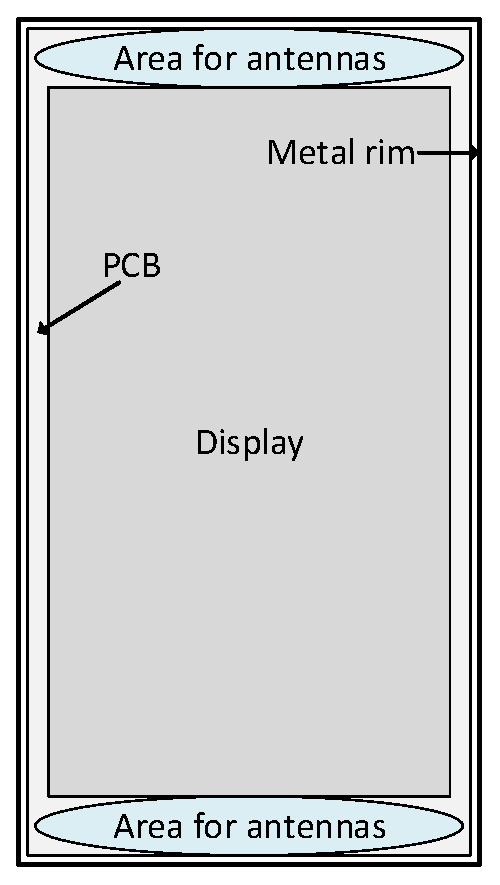
\includegraphics[width=0.9\textwidth]{img/metal_rim.eps}
        \caption{Typical locations of antennas in metal-rimmed handsets presented in \cite{ban_low_profile}.}
        \label{fig:metal_rim}
    \end{subfigure}
    \hspace{20pt}
    \begin{subfigure}[b]{0.4\textwidth}
        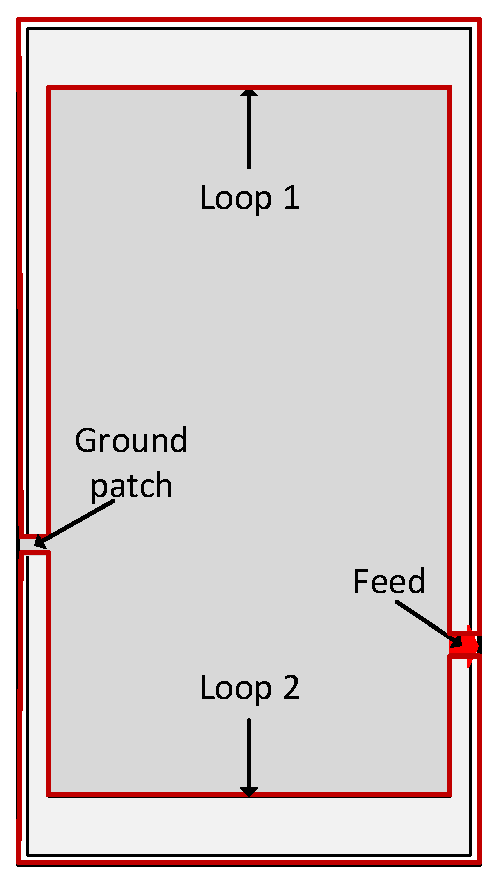
\includegraphics[width=0.9\textwidth]{img/dual_loop.eps}
        \caption{Example of a dual-loop antenna in metal-framed phone used in \cite{ban_dual_loop, stanley_lte_mimo}.}
        \label{fig:dual_loop}
    \end{subfigure}
    \caption{Proposed configurations in previous studies.}
    \label{fig:metal_rim_examples}
\end{figure}

As the display is acting as ground plane, the metal rim can be grounded with a small patch \cite{ban_dual_loop, stanley_lte_mimo}. Placing feed to another patch forms two loops between the display and the metal rim, as Figure \ref{fig:dual_loop} illustrates. This technique allows to keep the metal rim unbroken to maximize the strength of the phone. The length of the loop can be chosen such that different wave modes are excited. Since one feed-ground patch pair creates two loops of different lengths, both having own excited loop modes, this design can cover multiple frequency bands. %\cite{ban_dual_loop, stanley_lte_mimo}

Different resonant modes can be obtained also with slots in the ground plane \cite{yuan_slot}. Combining slots with loops a large number of resonance modes can be achieved \cite{hsu_compact}. Each element supports several modes that can be excited simultaneously to obtain wide bandwidth. However, slots and loops require quite large space, which is already limited. Monopole antenna in the side metal itself saves space inside the phone for other applications \cite{lee_monopole}. Cutting gaps to the metal rim constructs a monopole antenna, which couples with the rest of the rim to cover a wide set of frequencies \cite{chen_metal_frame}. %\cite{hsu_compact, yuan_slot, lee_monopole, chen_metal_frame}

\subsection{Full metal-covered handsets}
\label{sec:full_cover}
From the metal rim on the sides of the phone, the next step is metallic back cover. Similarly to handsets with metal rim, metallic back cover improves robustness but deteriorates the performance of antennas. However, the harmful effects of full metal back cover are so strong, that many of the antenna solutions in the recent studies have slots in the cover (Figure \ref{fig:metal_covers}). In those studies antennas are either PIFAs, or monopoles or the slots themselves \cite{wu_pier, son_wideband_mimo, wu_tunable, zhong_pier}. 

Few studies have still shown promising antenna designs for handsets with full metal back cover. These designs are based on PIFAs or L-shaped strips, but they require a part of the metal rim to be removed \cite{chen_compact_lte, wu_pier}. These modifications make the handset not fully metal-covered, but as the metallic back cover is the main challenge in these cases, the proposed solutions are usable as they have achieved at least 40\,\% efficiency in the operating bands. %\cite{chen_compact_lte, wu_pier}

\begin{figure}[H]
\centering
    \begin{subfigure}[b]{0.3\textwidth}
        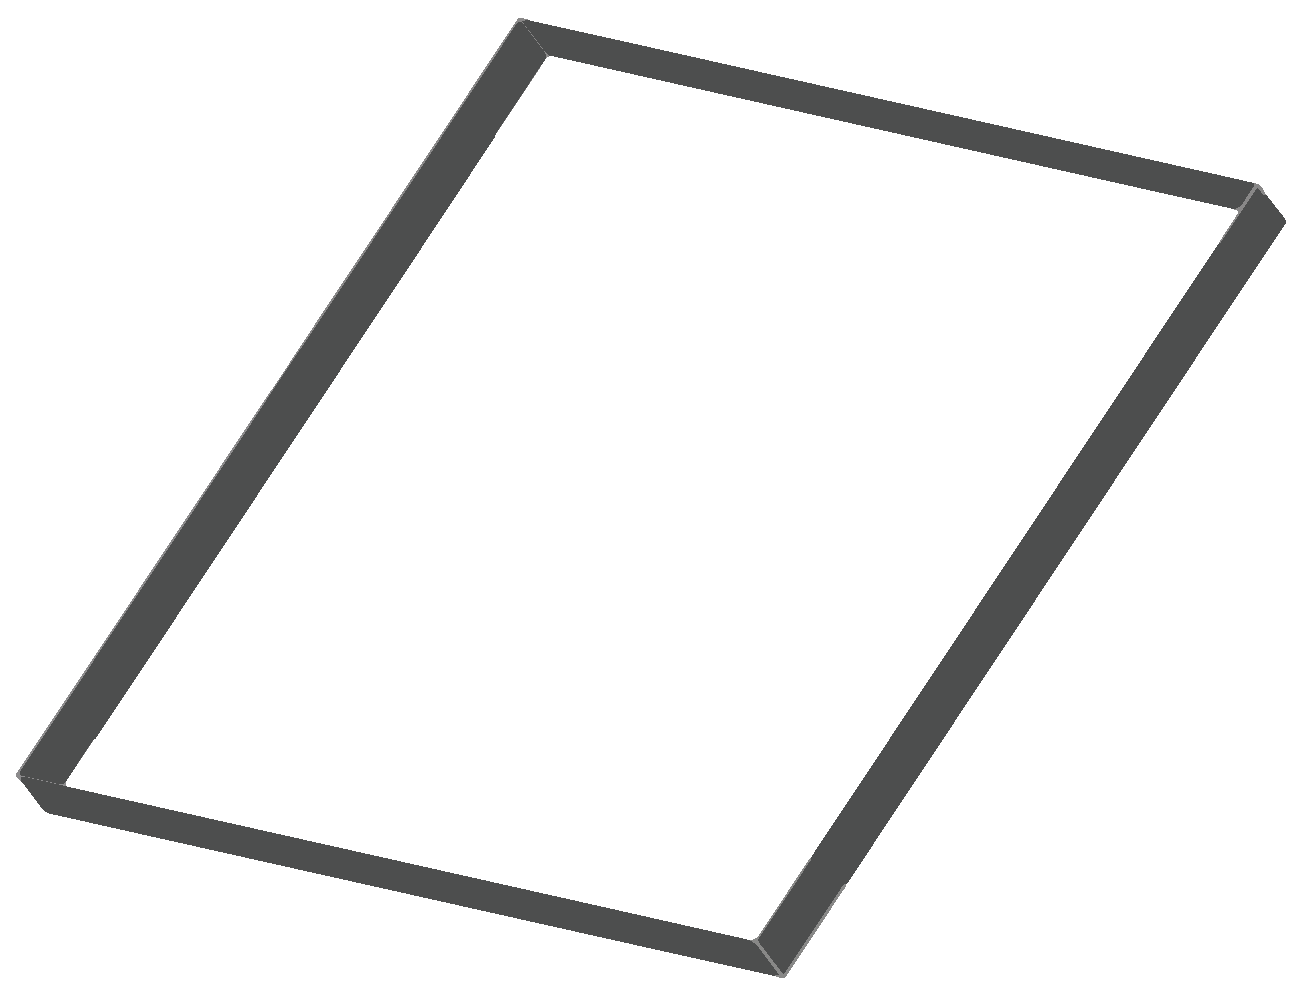
\includegraphics[width=\textwidth]{img/metal_rim2.eps}
        \caption{Metal rim.}
        \label{fig:rim}
    \end{subfigure}
    \begin{subfigure}[b]{0.3\textwidth}
        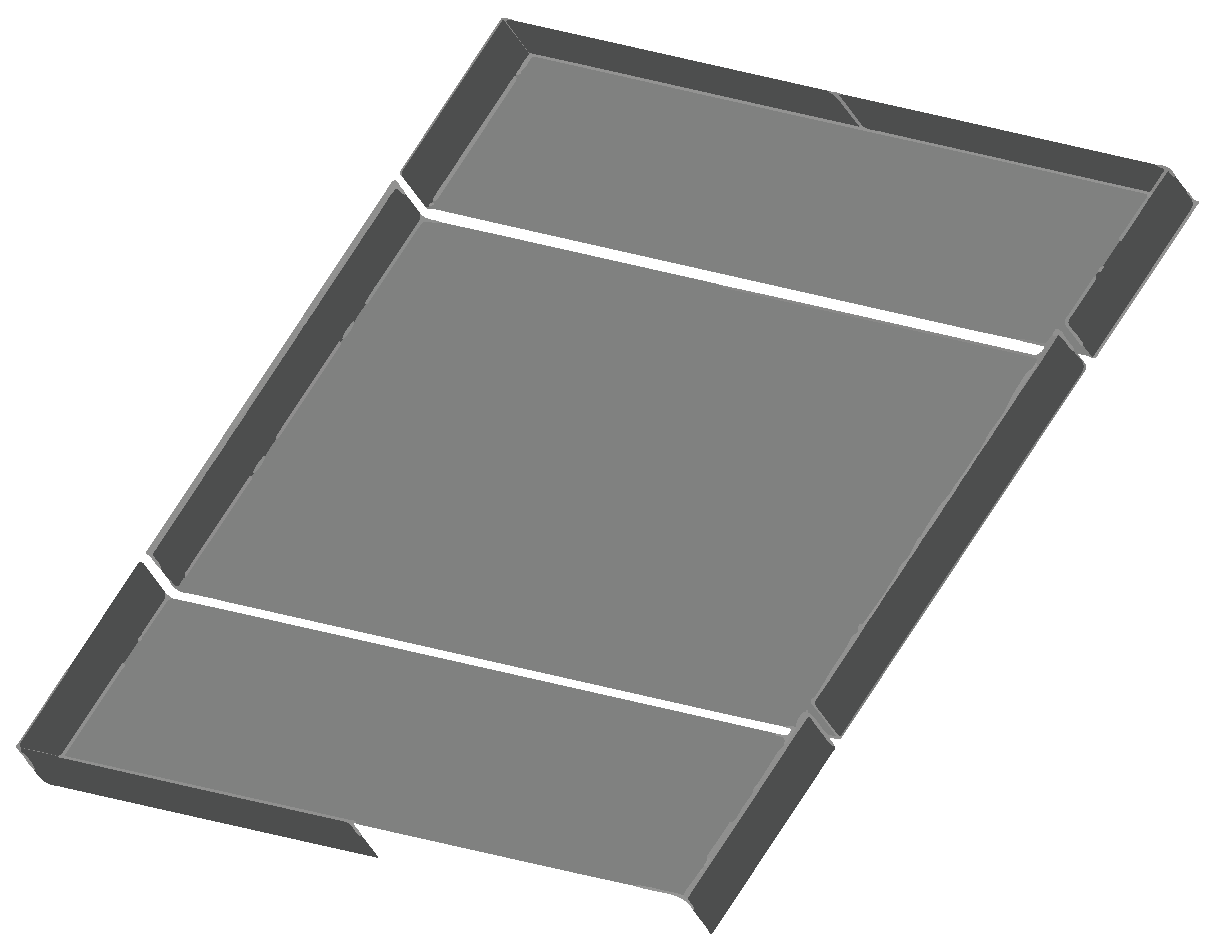
\includegraphics[width=\textwidth]{img/metal_cover_slots.eps}
        \caption{Examples of slots.}
        \label{fig:cover_slots}
    \end{subfigure}
    \begin{subfigure}[b]{0.3\textwidth}
        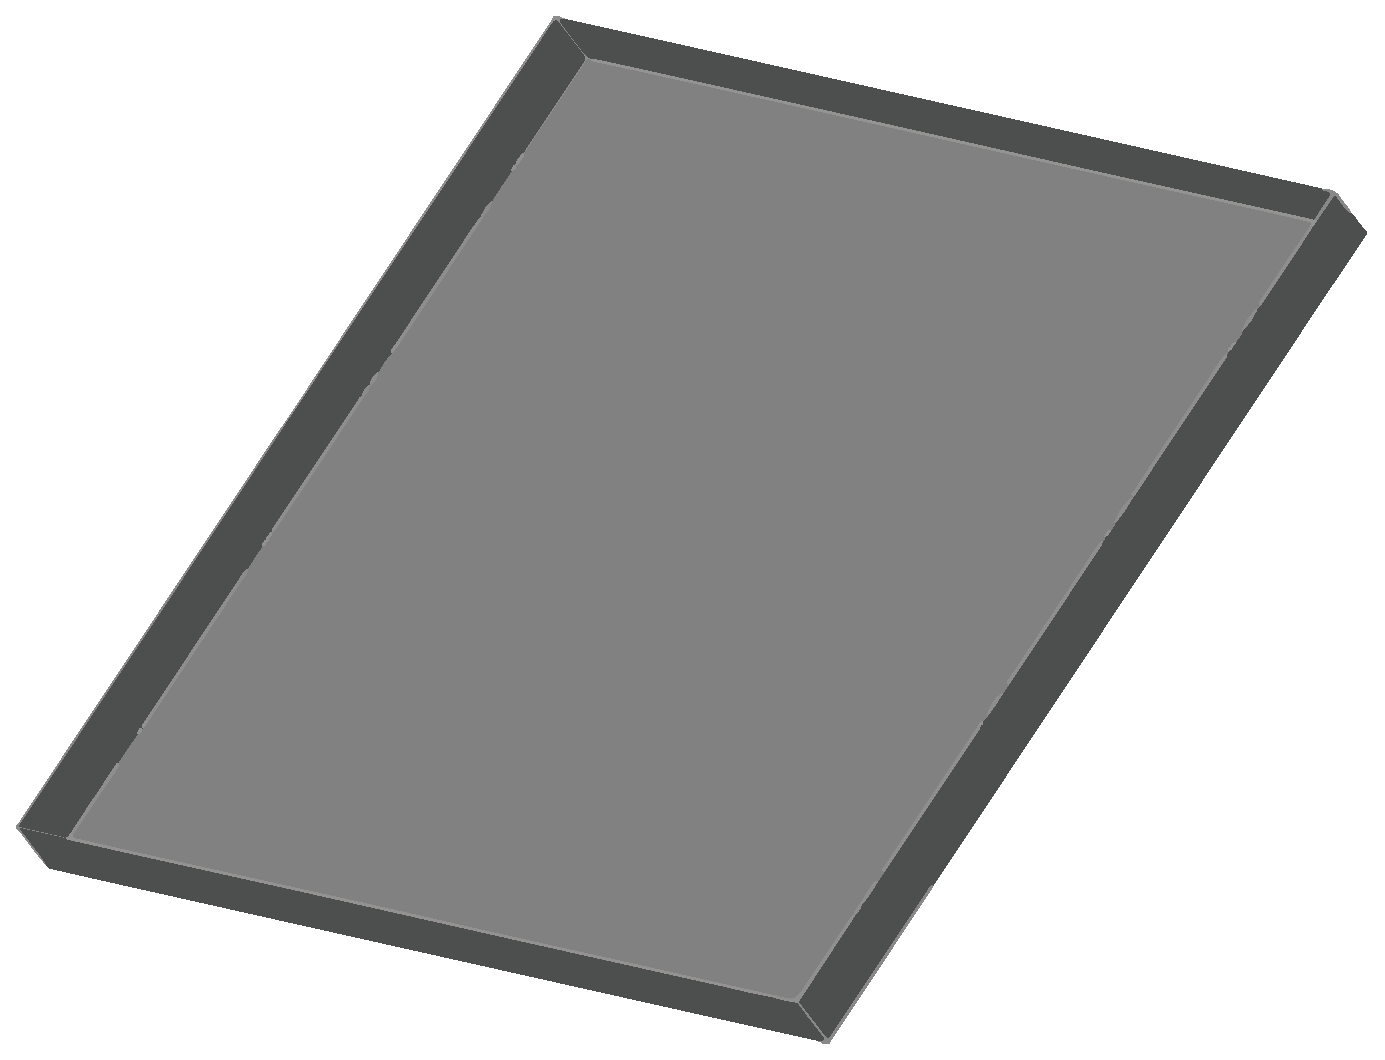
\includegraphics[width=\textwidth]{img/metal_cover_full.eps}
        \caption{Full metal cover.}
        \label{fig:full_cover}
    \end{subfigure}
    \caption{Re-illustrated examples of metal-covering of mobile phone presented in\cite{chen_compact_lte}.}
    \label{fig:metal_covers}
\end{figure}



\subsection{Key aspects in previous studies}
\label{sec:key_aspects}
More interesting matter in the previously studied antenna solutions is the technical details like operational frequencies and matching techniques, rather than positioning of antennas. As can be expected of today's mobile devices, all solutions are for LTE networks. Still, only antennas proposed in \cite{stanley_lte_mimo, son_wideband_mimo, chen_compact_lte, chen_metal_frame} support LTE bands operating at $700-800\,\mega\hertz$. These solutions tend to have average of $40\,\%$ efficiency in the low band. 

As majority of proposed solutions operate at frequencies $800-906\,\mega\hertz$ and $1.7-2.7\,\giga\hertz$, the performance of antennas in these ranges is obviously better. Typical efficiencies for lower frequencies are around $50-70\,\%$ on average and for the high band $60-80\,\%$ on average \cite{ban_dual_loop,chen_compact_lte,son_wideband_mimo,chen_metal_frame,zhong_pier}. Effect of user's hand or head is also measured in \cite{zhong_pier, chen_metal_frame,ban_dual_loop}. The effect is significant since efficiencies drop to average of $10-30\,\%$ in all supported bands. 

Handsets with metal covers and/or frames create a challenging operational environment for antennas. Besides the physical structure of an antenna, matching circuits have a major impact on final performance. Typically matching is done with lumped elements, and common amount of them is two or three for each antenna \cite{stanley_lte_mimo, zhong_pier, wu_pier}. Matching circuits improve isolation between elements leading to better element efficiency, as well as efficiency of the whole system. Even though wide band matching is desirable, it might be hard to achieve with fixed matching network. As resonance tends to occur in narrow peaks, digitally tunable capacitors (DTC) are used in antennas presented in \cite{chen_compact_lte,wu_tunable} to obtain good matching level over the whole band. To improve matching even further, few designs use band-stop \cite{lee_monopole, wu_pier} or band-pass \cite{chen_metal_frame} filters, or reactive loading \cite{chen_compact_lte, chen_metal_frame} to improve antenna's bandwidth. %\cite{stanley_lte_mimo, zhong_pier, lee_monopole, wu_pier, wu_tunable, chen_compact_lte}

The common feeding mechanism in different solutions is single-feed \cite{wu_tunable, chen_metal_frame, lee_monopole, chen_compact_lte}. That is, especially for designs with one element, but also for multiple elements. Designed slot or hybrid antennas have only one feeding point, and signal couples from fed element to others \cite{son_wideband_mimo,hsu_compact,zhong_pier,yuan_slot}. Also dual-loop antennas presented in \cite{stanley_lte_mimo,ban_dual_loop} have just one feed for both loops. However, in that case both loops are fed. Multiple feeds are used only in designs that have also other elements than slots or loops, or have the same antenna structure copied to the other end of the phone. Clearly, in those situations each element or structure is single-fed, but total number of feeds is plural \cite{stanley_lte_mimo, son_wideband_mimo}.

In LTE networks, one way to increase bandwidth and throughput is applying MIMO techniques in data transmission. However, MIMO operations are not that much studied for metal-covered phones. First design, seen in \cite{son_wideband_mimo}, has two similar antenna structures in both ends of the phone consisting complex monopole and planar inverted F antennas. This structure provides full MIMO capability for all operating frequencies, although antennas' efficiencies are only ca. $20\,\%$ at the lowest supported frequency of $746\,\mega\hertz$. The other MIMO solution proposed in \cite{stanley_lte_mimo} has a dual-loop antenna between ground plane and side metal frame, and a capacitive coupling element (CCE) antenna. Since the CCE antenna operates only on upper frequencies ($1710-2690\,\mega\hertz$) and does not cover the lower band, the design does not have full MIMO capability. %\cite{stanley_lte_mimo, son_wideband_mimo}


\begin{sidewaystable}[H]
%\begin{table}[H]
\centering
\caption{Comparison of previously studied antennas in metal-covered phones.}
\begin{tabular}{|M{0.08\textheight}|M{0.13\textheight}|M{0.09\textheight}|M{0.15\textheight}|M{0.13\textheight}|M{0.14\textheight}|M{0.16\textheight}|}
    \hline
    \textbf{Antenna} & \textbf{Antenna type} & \textbf{Size [$\milli\meter^2$]} & \textbf{Frequencies [$\mega\hertz$]} & \textbf{Efficiency [\%]} & \textbf{Matching network} & \textbf{Metal cover style}\\
    \hline
    \cite{ban_dual_loop} & Dual-loop & $10\times70$, $5\times70$ & $824-960$, $1710-2690$ & $60-80$ & N/A & Unbroken metal rim\\
    \hline
    \cite{hsu_compact} & U-shaped loop + T-shaped slot & $64\times8$ & $791-960$, $1710-2690$, $3410-3800$ & $50-90$ & N/A & Unbroken metal rim\\
    \hline
    \cite{yuan_slot} & Slot & $56.5\times15.5$ & $824-960$, $1710-2170$ & $60-80$ & N/A & Unbroken metal rim\\
    \hline
    \cite{stanley_lte_mimo} & Dual-loop + CCE & $10\times70$, $10\times70$, $12\times6$ & $698-960$, $1710-2690$ & $50-90$ & $\Pi$-topology for both antennas & Unbroken metal rim\\
    \hline
    \cite{lee_monopole} & Monopole & $50\times6.5$ & $824-960$, $1710-2690$ & $75-85$ & F-topology + band-stop filter & Metal rim\\
    \hline
    \cite{chen_metal_frame} & Monopole & $70\times5$ & $698-960$, $1710-2690$ & $50-70$ & 4 elements + band-pass filter + reactive loading & Metal rim\\
    \hline
    \cite{wu_pier} & Coupled monopoles & $20.5\times5$ & $1560-1690$, $2410-2490$, $4950-6510$ & average $40$ or $70$ & Band-stop filter & Full metal housing, with opening in the corner\\
    \hline
    \cite{son_wideband_mimo} & Monopole + IFA hybrid & $64\times16$, $64\times16$ & $746-960$, $1710-2170$, $2300-2400$ & $20-70$ & N/A & Metal back cover with slots\\
    \hline
    \cite{wu_tunable} & ILA & $35\times8$ & $824-960$, $1710-2170$ & $30-55$ & 2 elements + DTC & Full metal cover with slots\\
    \hline
    \cite{zhong_pier} & Slot & $65+20\times1$, $65\times1$, $40\times1$, $48\times1$ & $824-960$, $1560-1690$, $1710-2170$, $2410-2490$ & $40-65$ & 2 elements & Full metal cover with slots\\
    \hline
    \cite{chen_compact_lte} & Loop & $64\times8$ & $700-960$, $1710-2170$ & average $45$ or $60$ & 3 elements + 2 DTCs & Full metal housing with opening at the end of the phone\\
    \hline
\end{tabular}
%\end{table}
\end{sidewaystable}

\clearpage

%\section{Tutkimusaineisto ja -menetelmät}
\section{Design process \& methods}
\label{sec:objectives}
After introducing the former results of metal-covered handsets, the focus moves now to the new results achieved in this thesis work. This section presents the targets of this thesis in more detail, as well as the methods for answering the research question and solving the defined problems. The last part of this section contains the results from the first, preliminary simulations to gather information for the actual antenna design process.

\subsection{Design objectives \& strategy}
\label{sec:strategy}
The objective of this thesis is to study feasible antenna structures for metal-covered mobile phones. The phone should have two similar cellular antennas (main and diversity) for MIMO operation. Additionally, two antennas to operate on GPS and Wi-Fi frequencies are to be designed. To clarify, from now on, main antenna refers to the first cellular antenna to be designed, and diversity antenna to the second one, regardless how their final performances will compare to each other. Table \ref{tab:design_goals} below presents the goals and requirements for this project.

\begin{table}[H]
    \centering
    \caption{Criteria for the antennas to be designed.}
    \label{tab:design_goals}
    \begin{tabular}{|l|c|}
        \hline
         \textbf{Parameter} & \textbf{Value} \\
         \hline
         Reflection coefficient & $S_{11} < -5\,\db$\\
         \hline
         Cellular efficiency & $\eta > 30\,\%$\\
         \hline
         Isolation between main and diversity antenna & $S_{21} < -15\,\db$\\
         \hline
         GPS/Wi-Fi efficiency & $\eta > 40\,\%$\\
         \hline\hline
         \textbf{Frequencies} & \\
         \hline
         Main cellular antenna & $0.704-0.960\,\giga\hertz, 1.71-2.69\,\giga\hertz$\\
         \hline
         Diversity cellular antenna & $0.704-0.960\,\giga\hertz, 1.71-2.69\,\giga\hertz$\\
         \hline
         GPS antenna & $1.56-1.61\,\giga\hertz$\\
         \hline
         Wi-Fi antenna & $2.4-2.484\,\giga\hertz, 5.15-5.875\,\giga\hertz$\\
         \hline
    \end{tabular}
\end{table}

Electromagnetic (EM) simulations were made in CST Microwave Studio \cite{cst} (later CST). It was used to create antenna and phone models, and to calculate system's $S$-parameters. Simulations were focused on antenna's initial matching, i.e. $S_{ii}$ for each antenna. The procedure of testing different antenna structures was pretty straightforward: first a model was built, then simulated, and finally the obtained results were analyzed. Analysis focuses on the frequencies of the resonances, their bandwidths, and matching levels. If the combination of these three parameters looks promising (e.g.\ sufficient levels and rather wide band), a matching circuit is constructed to enhance the performance. Based on the previous findings, the model was modified aiming to wide impedance matching, and then simulated again. The first tests were done with a simple model and a simple antenna design. While the antenna structures got better, the model of the phone was also modified to be more realistic.

Antennas were designed in order of significance. The cellular antennas were considered more important as they operate on the lowest frequencies, and therefore require the largest space. Thus, they were studied first. Development process of the antennas began with the main antenna, and when it was operating properly, the same process was applied to design the diversity antenna. The final step was to add solutions for GPS and Wi-Fi antennas. Figure \ref{fig:ant_order} illustrates the proceeding order. 

The basic research strategy was first to find solution for the main antenna to operate on the low band (LB, $704-960\,\mega\hertz$). Lower band was designed first, since it is harder to reach the determined matching levels and efficiencies at lower frequencies. Results from the previous studies have shown weaker performance at those areas. Also, the required antenna structures are larger, which makes them more critical to be prioritized due to the already limited available space. After a reasonable performance was achieved at that band, the model was configured to support also the high band (HB, $1.71-2.69\,\giga\hertz$). Accordingly, the design of GPS/Wi-Fi antennas was started from the lowest frequency, i.e.\ GPS ($1.56-1.61\,\giga\hertz$), after which, the Wi-Fi frequencies ($2.4-2.484\,\giga\hertz$ and $5.15-5.875\,\giga\hertz$) were added. The process flow of designing one antenna is visualized in Figure \ref{fig:ant_design}.

Before moving on the next antenna, the design constraints had to be checked. One antenna was iterated until the targets were reached (Figure \ref{fig:step}). When the antenna under development was performing according to the requirements, or at least at a decent level, the design of a another antenna was started.

Designing antennas was not limited only in antenna structures. In order to reach the goals presented above, matching networks were to be designed as well. Finding usable circuit topologies was done simultaneously with EM simulations. Optenni Lab \cite{optenni} and NI AWR Design Environment \cite{awr} (later AWR) were used for this purpose. The $S$-parameter file obtained from CST-simulations was given to and read by these programs. Optenni Lab searches for the best matching circuit according to given frequency band settings and amount of circuit elements. Resulted circuits were modified and fine-tuned in AWR, to reach the defined design objectives. Also, in AWR the ideal circuit elements were later replaced with models of actual components to obtain more realistic results.

\begin{figure}[H]
    \centering
    \begin{subfigure}[b]{\textwidth}
        \begin{tikzpicture}[node distance=2cm]
            \node (main) [ant] {Main antenna};
            \node (div) [ant, right of=main, xshift=2cm] {Diversity antenna};
            \node (gps1) [ant, right of=div, xshift=2cm] {GPS/Wi-Fi antenna 1};
            \node (gps2) [ant, right of=gps1, xshift=2cm] {GPS/Wi-Fi antenna 2};
            \draw [arrow] (main) -- (div);
            \draw [arrow] (div) -- (gps1);
            \draw [arrow] (gps1) -- (gps2);
        \end{tikzpicture}
        \caption{Design order of the required antennas.}
        \label{fig:ant_order}
    \end{subfigure}
    
    \begin{subfigure}[b]{\textwidth}
        \begin{tikzpicture}[node distance=2cm]
            \node (ant) [ant] {New antenna};
            \node (que) [query, right of=ant, xshift=2cm] {Antenna type};
            \node (lb) [block, right of=que, xshift=0.5cm, yshift=-1.5cm] {LB};
            \node (hb) [block, right of=lb, xshift=0.5cm] {HB};
            \node (mc) [block, right of=hb, xshift=0.5cm] {MC};
            \node (gps) [block, right of=que, xshift=0.5cm, yshift=1.5cm] {GPS};
            \node (wifi24) [block, right of=gps, xshift=0.5cm] {2.4\,GHz};
            \node (wifi5) [block, right of=wifi24, xshift=0.5cm] {5\,GHz};
            \draw [arrow] (ant) -- (que);
            \draw [arrow] (que) |- node[anchor=north] {cellular} (lb);
            \draw [arrow] (lb) -- (hb);
            \draw [arrow] (hb) -- (mc);
            \draw [arrow] (que) |- node[anchor=south] {GPS/Wi-Fi} (gps);
            \draw [arrow] (gps) -- (wifi24);
            \draw [arrow] (wifi24) -- (wifi5);
            \draw [arrow] (wifi5) -- (mc);
            \draw [arrow] (mc) -- +(0,-1) -| (ant);
        \end{tikzpicture}
        \caption{Design process of an antenna.}
        \label{fig:ant_design}
    \end{subfigure}
\end{figure}  

\begin{figure}[H]
    \centering
    \ContinuedFloat
    \begin{subfigure}[b]{\textwidth}
        \begin{tikzpicture}[node distance=2cm]
            \node (ant) [ant] {Antenna to design};
            \node (que) [query, right of=ant, xshift=2cm] {Targets reached?};
            \node (ant2) [ant, right of=que, xshift=3cm] {Next antenna};
            \draw [arrow] (ant) -- (que);
            \draw [arrow] (que) -- node[anchor=south] {yes} (ant2);
            \draw [arrow] (que) -- +(0,-2.5)-| (ant)  node[near start,sloped,below] {no} ;
        \end{tikzpicture}
        \caption{A single step of the whole process.}
        \label{fig:step}
    \end{subfigure}
    \caption{Flowcharts illustrating the design procedure.}
    \label{fig:flowcharts}
\end{figure}


\subsection{Electromagnetic model of the mobile phone}
\label{sec:phone}
Besides the antennas, also the phone had to be modeled electromagnetically. For this project it was specified to use a mechanically accurate model, shown in Figure \ref{fig:cad}. However, this model is too detailed for research purposes, and thus it will be modified, which is explained more in Section \ref{sec:sim_realistic}. The model anyway consists of metallic back cover and side frame, plastic structure, and some subsystems of a phone. Metallic parts, and all of the subsystems and other parts were modeled as perfect electric conductors (PEC) to reduce simulation times. The plastic rim was the only non-metallic part of the model.
\begin{figure}[H]
    \centering
    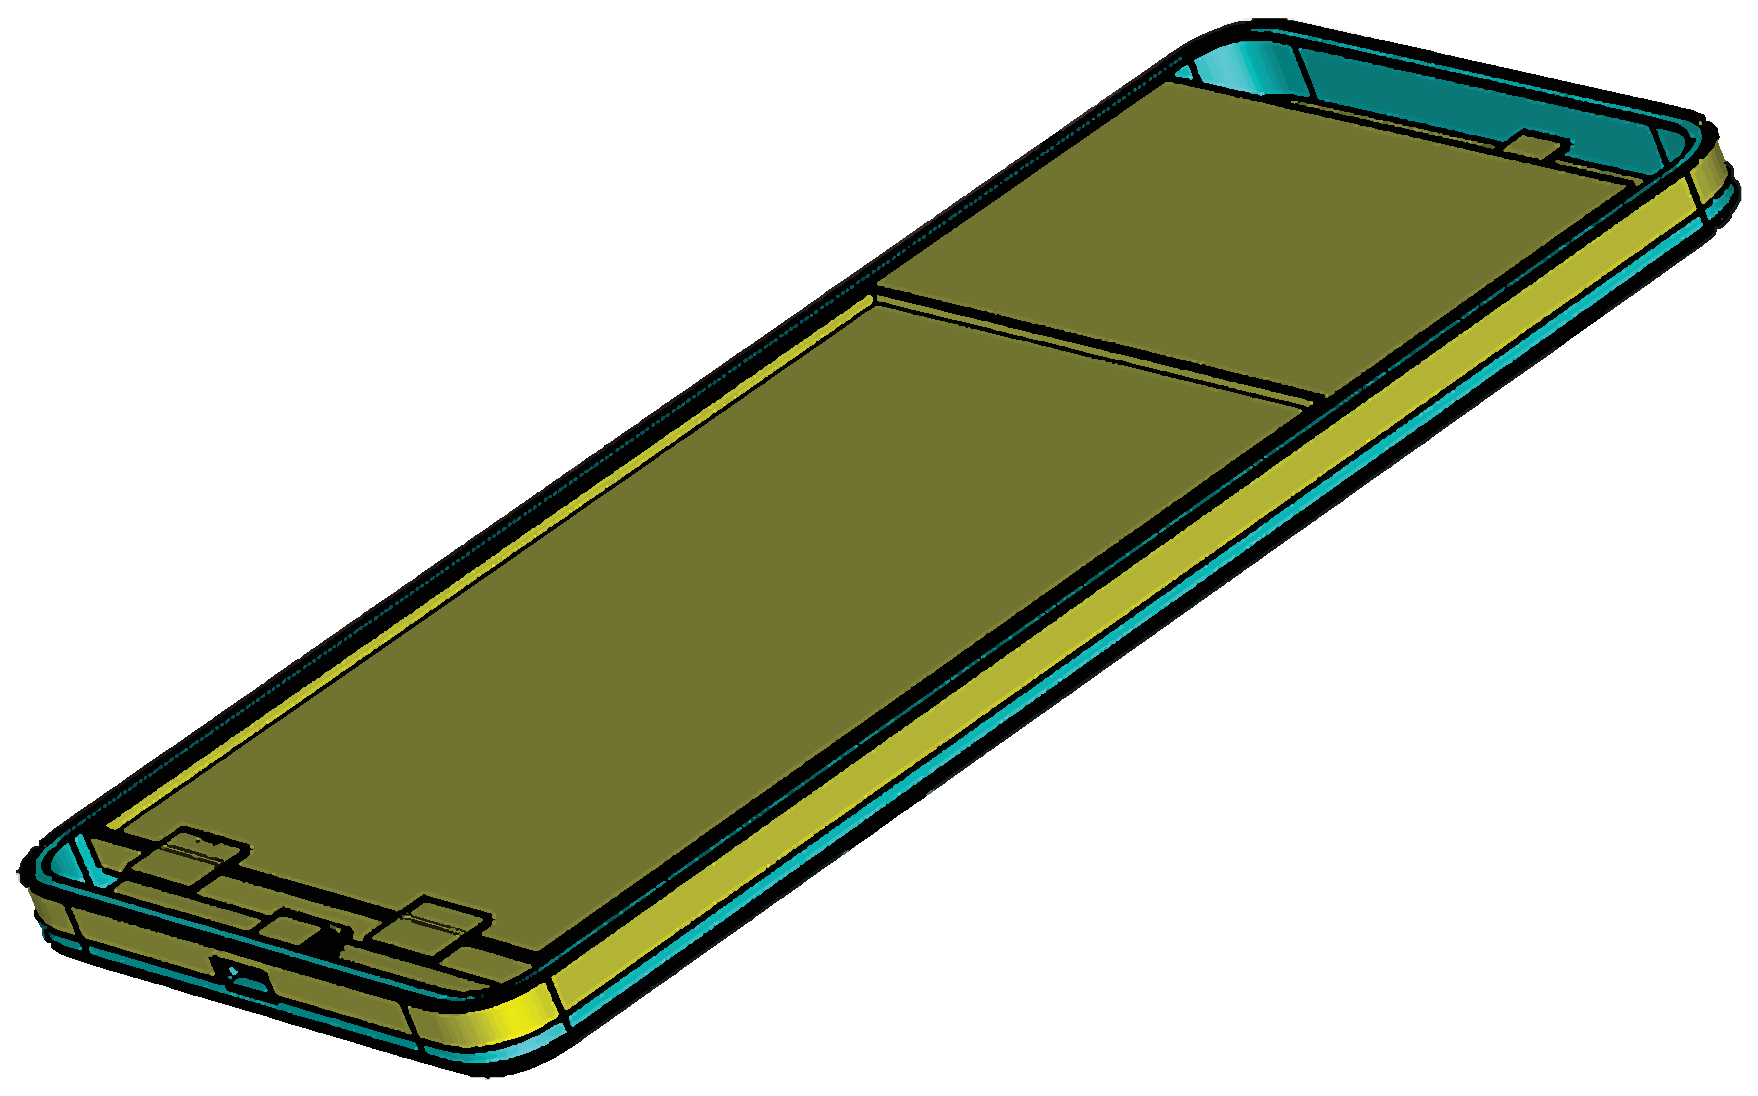
\includegraphics[width=0.6\textwidth]{img/cad.eps}
    \caption{3D-model of a smart phone.}
    \label{fig:cad}
\end{figure}

Before the precise model was taken into use, simulations were first done with a plain model. Basically, that was a PEC-sheet for back cover, and a FR4-substrate with a another PEC-sheet to model the display. Figure \ref{fig:basic_structure} illustrates that model, with the key dimensions of the phone marked into it. The antennas were built to the empty sides of the model, and eventually they would be integrated to the side frame of the accurate model. The simple model was used until a promising structure for the main antenna was found. 
\begin{figure}[H]
    \centering
    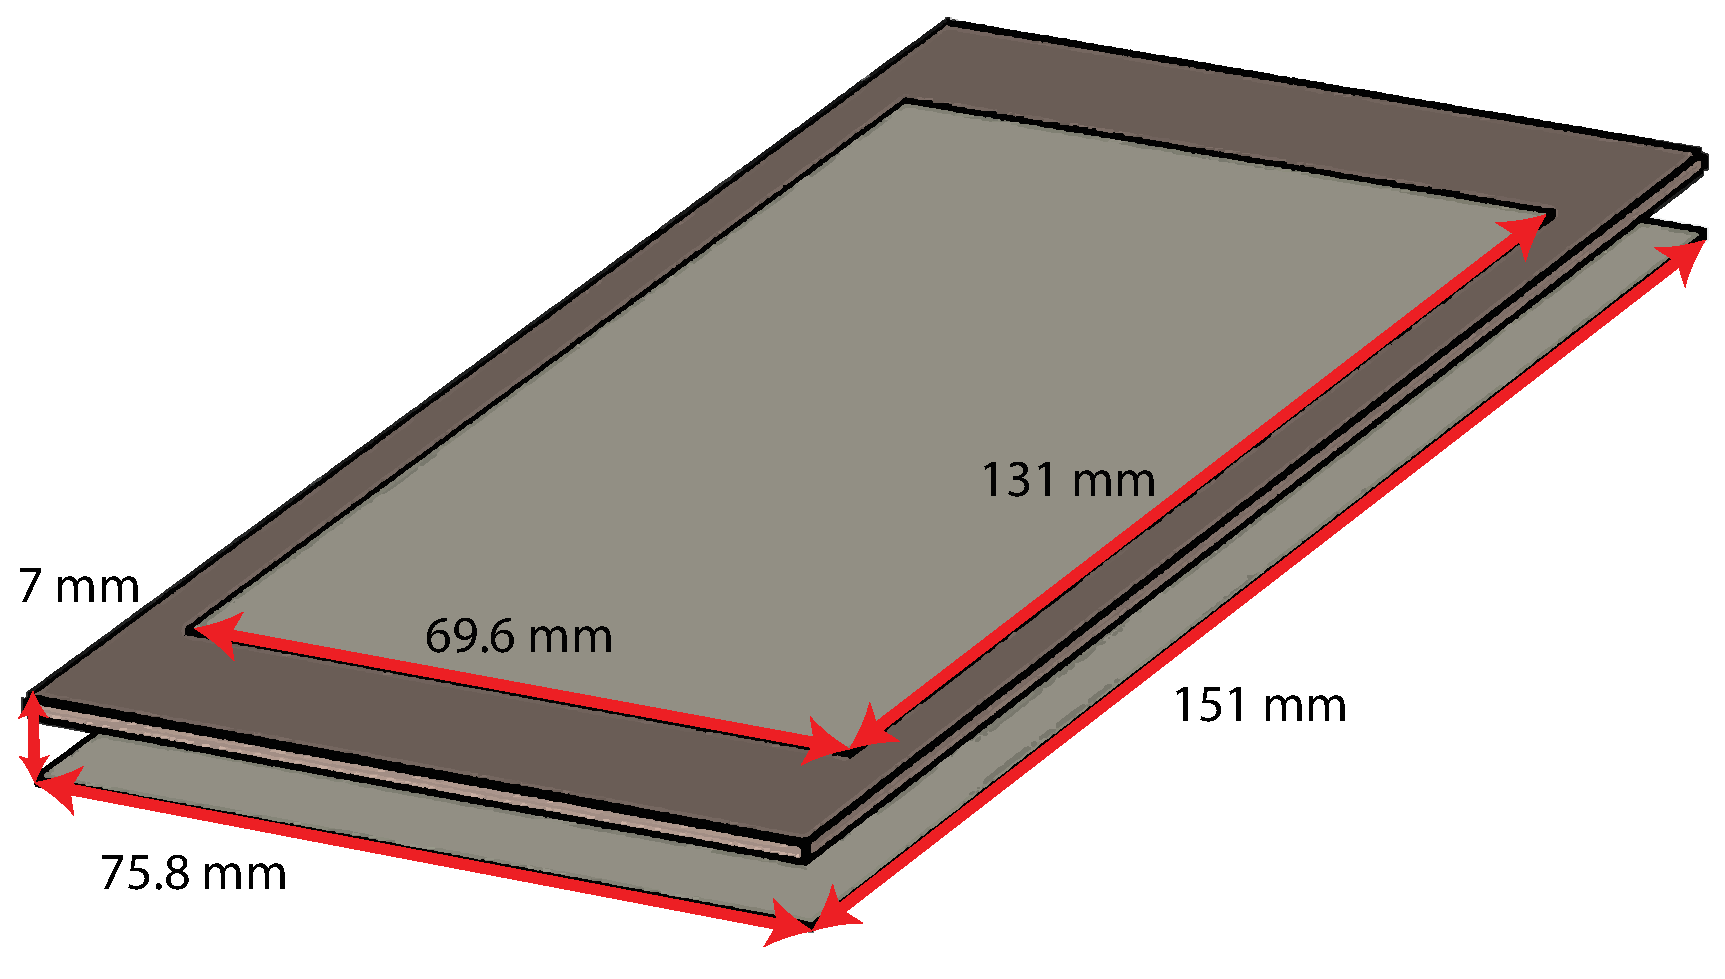
\includegraphics[width=0.6\textwidth]{img/basic_structure.eps}
    \caption{Simplified, basic model of a mobile phone to be used in simulations.}
    \label{fig:basic_structure}
\end{figure}

\subsection{Preliminary antenna study}
\label{sec:pre_study}
The first simulations with the plain model were about gathering knowledge on how different structures perform in the presence of the metal cover. Gaining this information was critical since antennas in metal-covered mobile phones are not that much studied, as was presented in Section \ref{sec:metal_rim}. This preliminary study (later also pre-study) focuses on different dimensions of antennas, their locations, shapes, feed positions, and the metal cover itself. The structures of antenna elements were kept as simple as possible in order to follow the effects of each parameter in an efficient way. 


\subsubsection{Effect of the metal cover}
\label{sec:metal_effect}
The main point of interest, as well as the main challenge, is the metal cover and how it affects the antenna's performance. To demonstrate the challenge of this design project, simulations to test the effect of the metal were run. Since this test was just an example, simulation model was kept simple. A long, L-shaped antenna completely covering one long side and one short side, with a little square on the corner was used in this test. Models are shown in Figure \ref{fig:metal_vs_nometal_model}.

\begin{figure}[H]
    \centering
    \begin{subfigure}[b]{0.49\textwidth}
    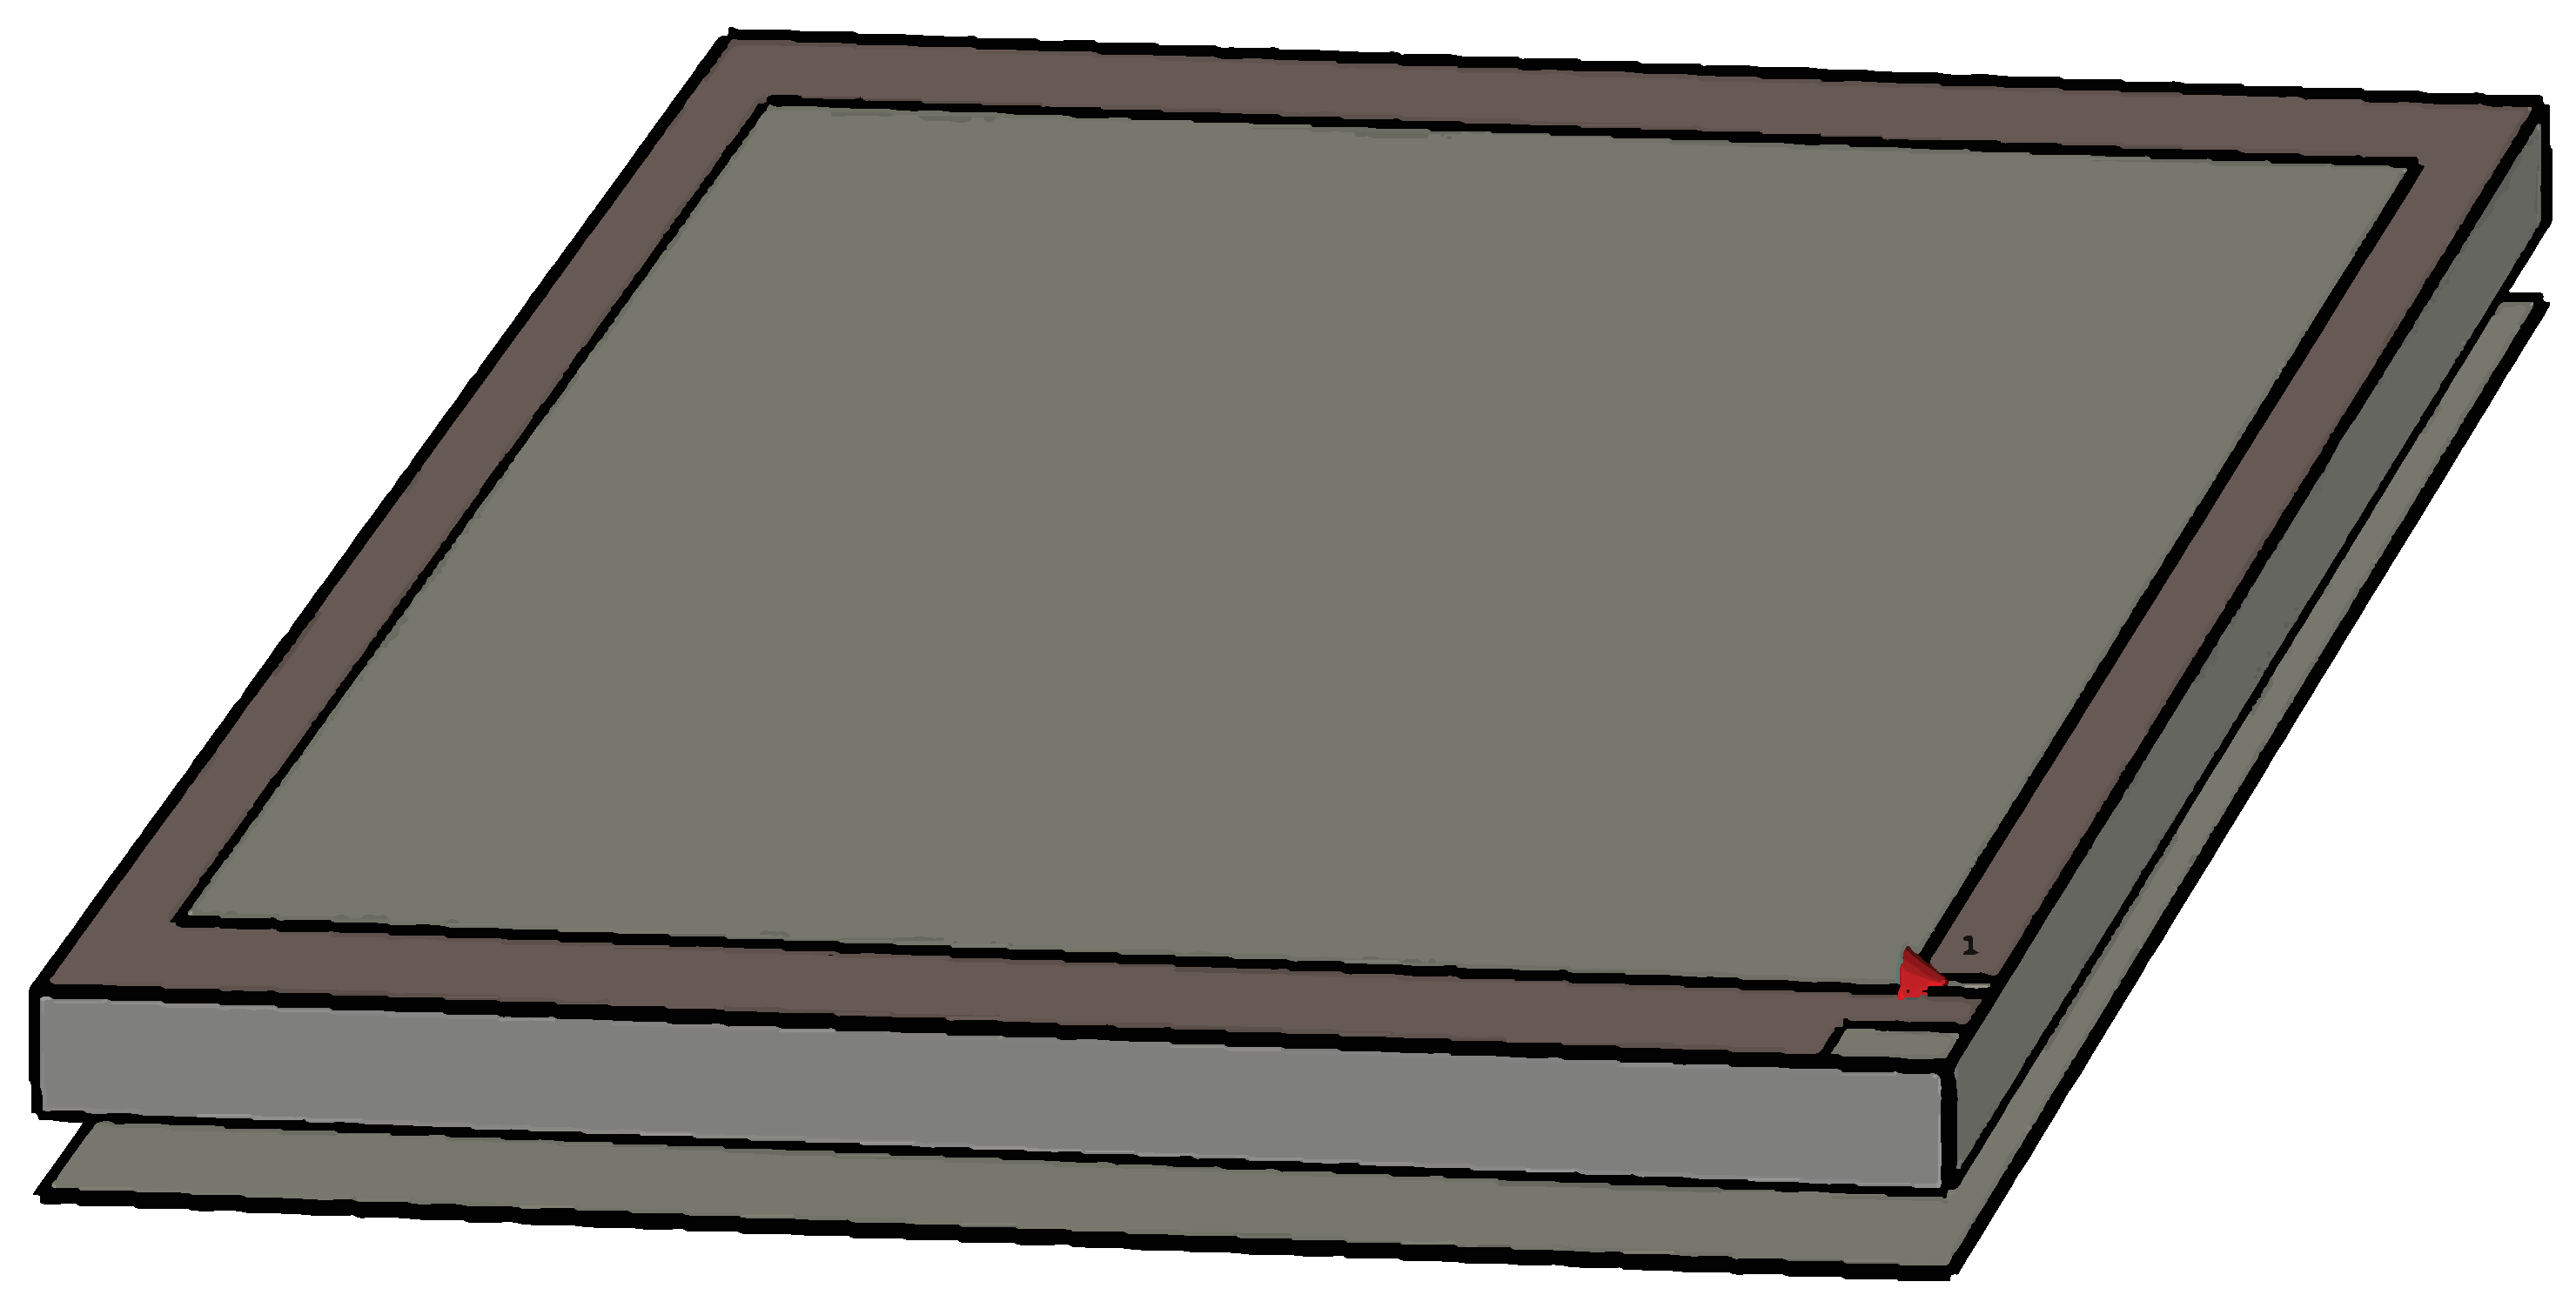
\includegraphics[width=\textwidth]{img/metal_cover.eps}
    \caption{With metal cover.}
    \label{fig:metal_cover}
    \end{subfigure}
    \begin{subfigure}[b]{0.49\textwidth}
    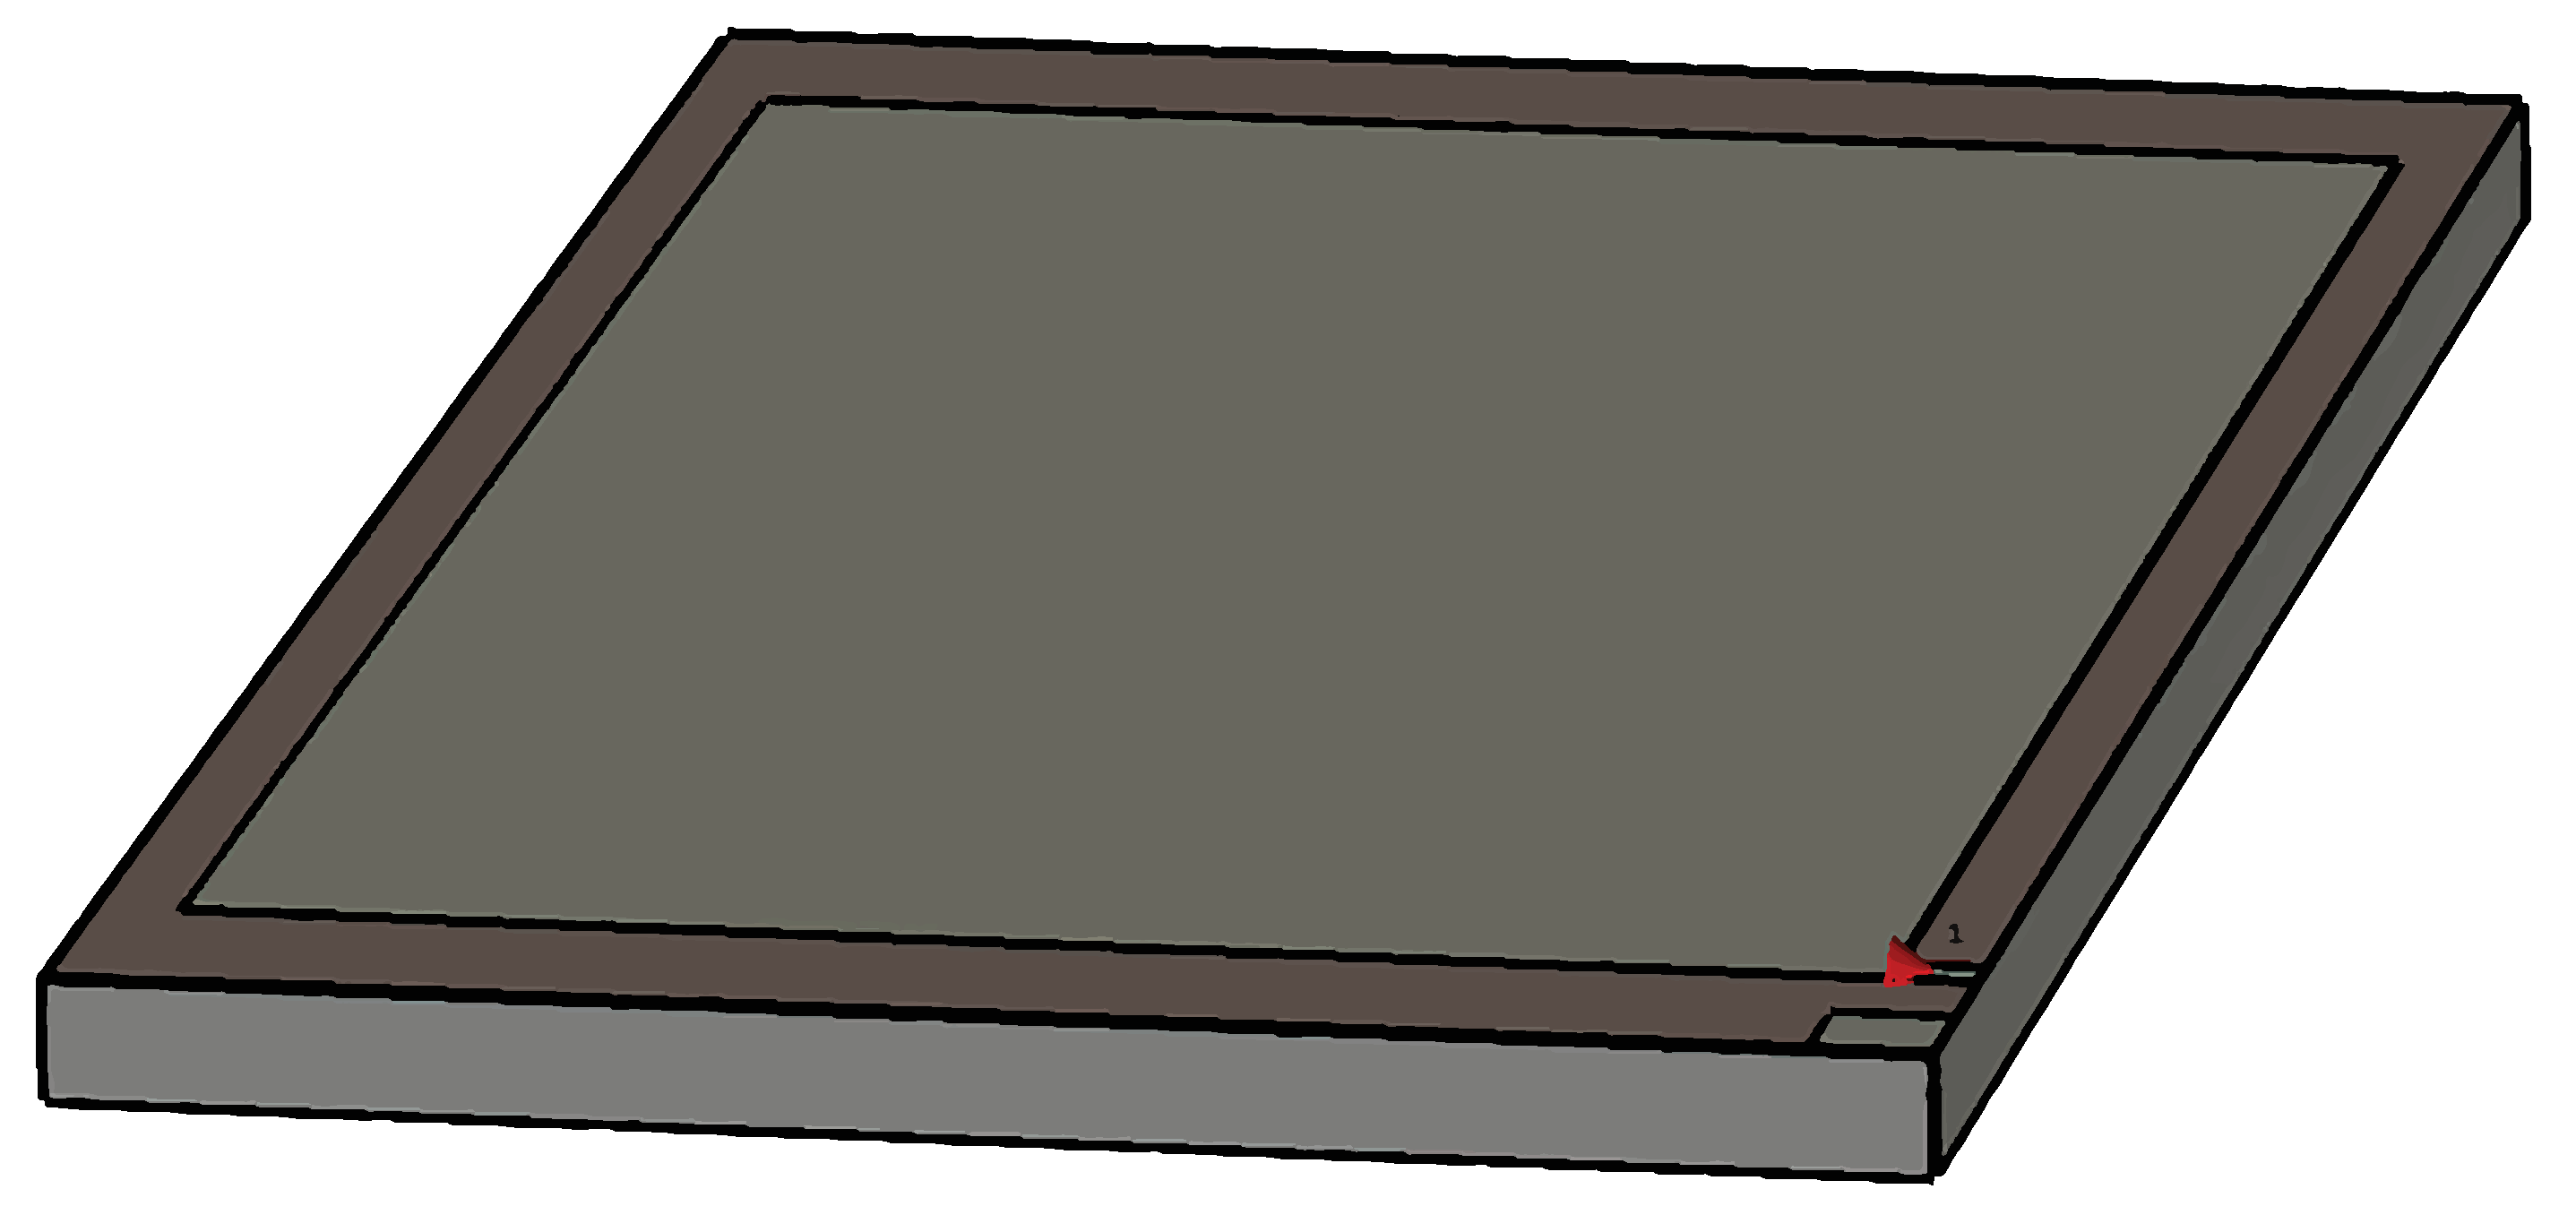
\includegraphics[width=\textwidth]{img/no_metal_cover.eps}
    \caption{Without metal cover.}
    \label{fig:nometal_cover}
    \end{subfigure}
    \caption{Simulation models used to test the effect of metal cover. Antenna element is on the side of the phone.}
    \label{fig:metal_vs_nometal_model}
\end{figure}

Figure \ref{fig:metal_vs_nometal} shows clearly the effect of the metal cover. At the low band, the results reveal a major difference. The aim of the matching level $-5\,\db$ is almost achieved when the metal cover is taken away without any external matching networks. With the metal cover the antenna resonates more with narrower peaks and has no desired matching level at any frequency. 

Figure \ref{fig:metal_vs_nometal_matched} presents the same simulations with a four-element matching circuit designed with Optenni Lab. The software was set to generate matching circuits of four components, with $-5\,\db$ target efficiency. This time the difference is even larger. Without metal cover the desired matching level is exceeded by far. In contrary, adding matching circuit to the other case is not much of help. Even though the level is now more constant in the band, it is far from acceptable, and the difference of these cases is about $8\,\db$.

\begin{figure}[H]
    \centering 
    \begin{subfigure}[b]{0.49\textwidth}
        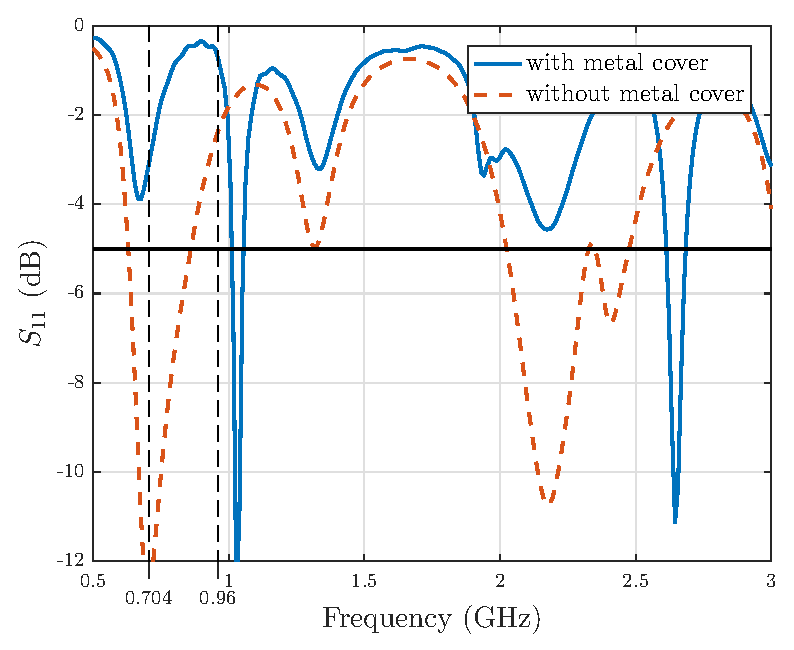
\includegraphics[width=\textwidth]{img/metal_vs_nometal.eps}
        \caption{Without matching circuit.}
        \label{fig:metal_vs_nometal}
    \end{subfigure}
    \begin{subfigure}[b]{0.49\textwidth}
        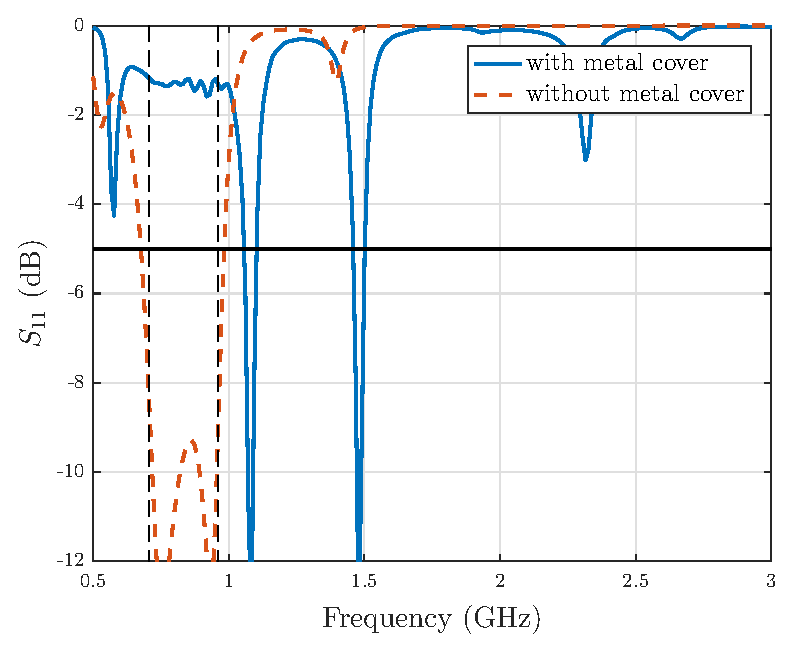
\includegraphics[width=\textwidth]{img/metal_vs_nometal_matched.eps}
        \caption{Matched antennas.}
        \label{fig:metal_vs_nometal_matched}
    \end{subfigure}
    \caption{Effect of the metal back cover on antenna performance.}
    \label{fig:metal_vs_nometal_results}
\end{figure}



\subsubsection{Size of an antenna}
\label{sec:antenna_size}
As mentioned earlier in Section \ref{sec:strategy}, antennas were designed and developed in the EM simulator. Each simulated design provided information that was useful for the following iterations. 

The first interesting metric to investigate was the size of the antenna. This meant length ($l$) and width ($w$) of the antenna since all elements were considered as thin metallic sheets. The tested antennas were $2\,\milli\meter$ wide metal strips either on the long or the short side of the phone (see Figures \ref{fig:ant_length_long} and \ref{fig:ant_length_short}, respectively). In both cases everything else was kept constant except the length of antenna. 

\begin{figure}[H]
    \centering
    \begin{subfigure}[b]{0.49\textwidth}
        \includegraphics[width=\textwidth]{img/length_long.eps}
        \caption{Antenna located on the side of the phone.}
        \label{fig:ant_length_long}
    \end{subfigure}
    
    \begin{subfigure}[b]{0.49\textwidth}
        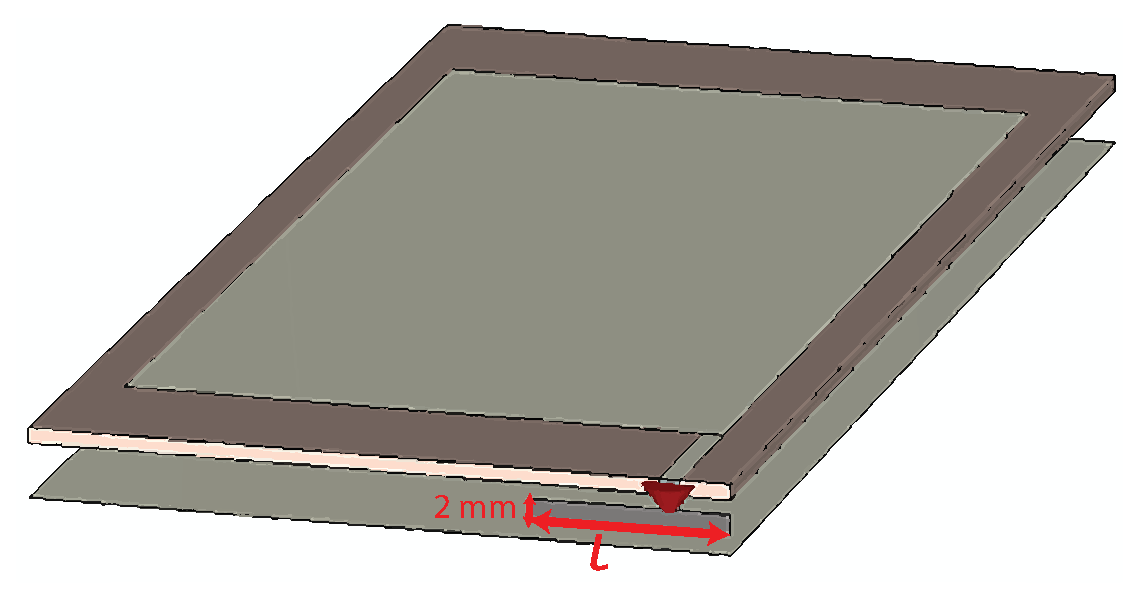
\includegraphics[width=\textwidth]{img/length_short.eps}
        \caption{Antenna located at the end of the phone.}
        \label{fig:ant_length_short}
    \end{subfigure}
    \caption{Models used to test the effect of antenna's length.}
    \label{fig:ant_length_model}
\end{figure}

Figure \ref{fig:ant_length_result} shows the effect of antenna length with five different values in both cases. Especially in the low band, none of these antennas is suitable. Anyhow, few observations can be made from these simulations. Looking at Figure \ref{fig:ant_length_long_res} reveals that resonance of the longest antenna is the weakest and shorter antennas are better matched near the low band. Shortest tested antenna, having length of $20\,\milli\meter$, has the most promising performance in the high band.

Effects of antenna's length are quite similar, if antenna is placed on the top end of the phone, like Figure \ref{fig:ant_length_short_res} presents. Again, none of the tested lengths fits for the low band, but this time the length does not make as clear difference. Each of the tested lengths has strong resonances near the low band at slightly different frequencies. Comparing the two cases at the low band, it seems that antenna located at the end of the phone operates better, and larger elements are slightly better than smaller ones.

\begin{figure}[H]
    \centering
    \begin{subfigure}[b]{0.49\textwidth}
        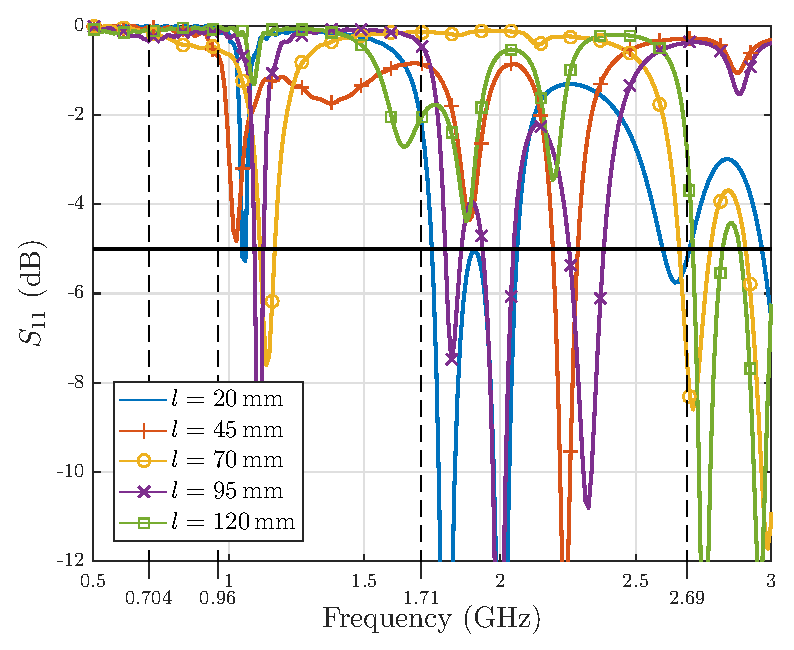
\includegraphics[width=\textwidth]{img/ant_length_long_res.eps}
        \caption{Antenna located on the side of the phone.}
        \label{fig:ant_length_long_res}
    \end{subfigure}
    \begin{subfigure}[b]{0.49\textwidth}
        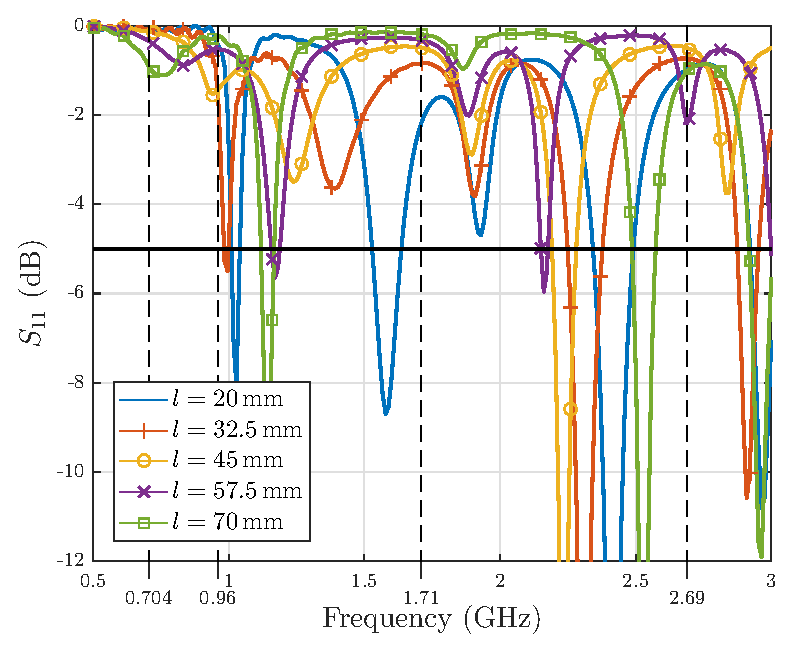
\includegraphics[width=\textwidth]{img/ant_length_short_res.eps}
        \caption{Antenna located on the top of the phone.}
        \label{fig:ant_length_short_res}
    \end{subfigure}
    \caption{The effect of antenna's length.}
    \label{fig:ant_length_result}
\end{figure}

The other issue affecting the size of an antenna besides length is its width. Impact of width is tested with the same structure that was used to test the effect of length, when the antenna is placed on the top of the phone. Antenna's length was also $70\,\milli\meter$ in this case. As Figure \ref{fig:width_res} presents, the effect of the width is quite minimal. Wider element gives a little bit better bandwidth in the both desired operational bands, but difference is not significant. Nevertheless the similarity of the results, larger bandwidth is more achievable with wider elements. Only it must be remembered, that the space for antennas is very limited on the sides of the phone, and thus, antennas cannot be much wider.

\begin{figure}[H]
    \centering
    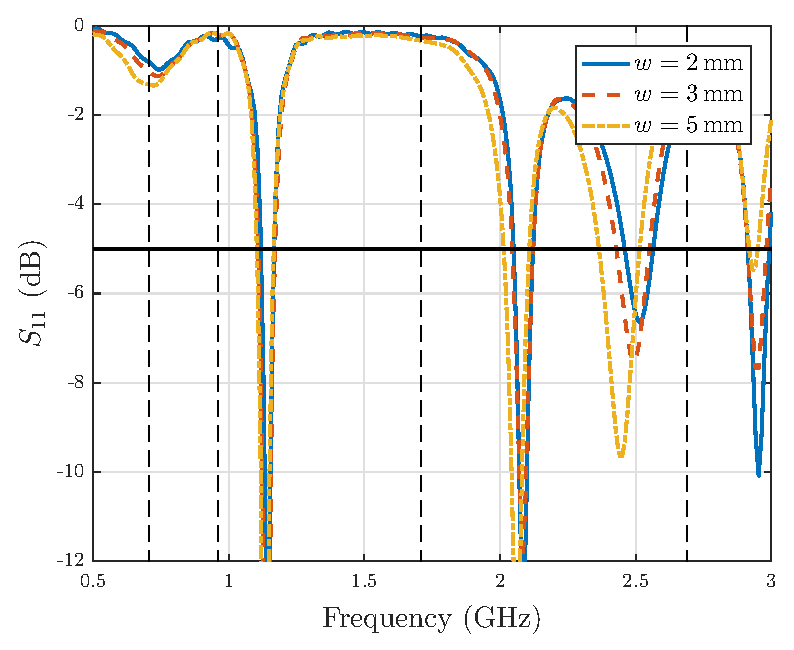
\includegraphics[width=0.5\textwidth]{img/width_res.eps}
    \caption{Effect of the width of an antenna.}
    \label{fig:width_res}
\end{figure}


\subsubsection{Location of the feed}
\label{sec:feed}
Besides the size of an antenna, another interesting parameter is the location of the feed. This is tested with the same structure that was used to test the impact of the metallic back cover except for the small block on the corner, shown in Figure \ref{fig:metal_cover} earlier. Feeds are located in two ways: either on the long or the short side, like in Figures \ref{fig:ant_length_long} and \ref{fig:ant_length_short}, respectively. The feed is placed between the antenna and the ground plane, or the display in this case, and four different locations are tested on each side. The first position is in the corner of the ground plane, and the last is in the center of it. Between these are two positions at equal distances, denoted as ground 1/3 and ground 2/3.

Figures \ref{fig:feed_pos_side_res} and \ref{fig:feed_pos_top_res} show the simulation results for feed on the long side and feed on top, respectively. Both of these graphs yield the same conclusion: for the low band, feed provides more promising operation when located at the corner of the ground plane. For the high band, feed location is the most promising when it is shifted away from the corner, and is located on the top side of the phone.

\begin{figure}[H]
    \centering
    \begin{subfigure}[b]{0.49\textwidth}
        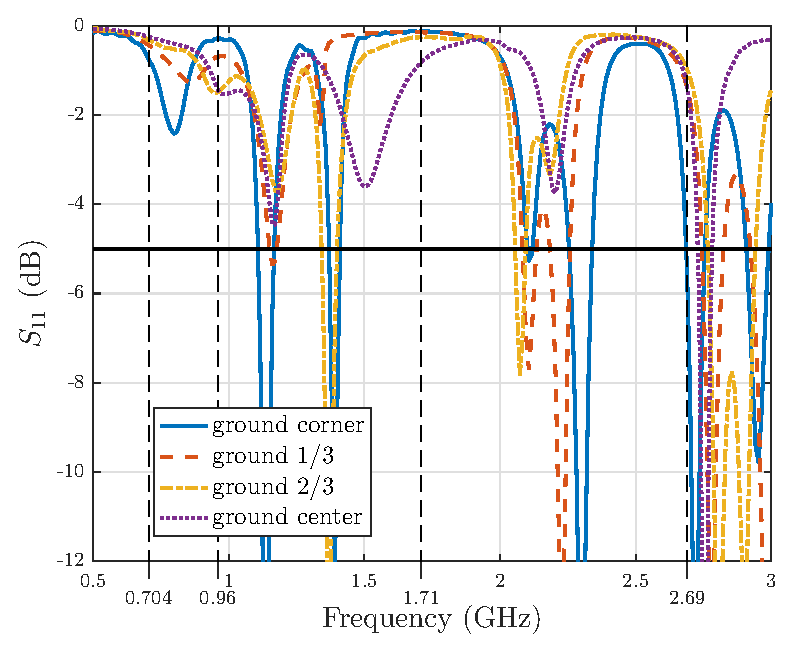
\includegraphics[width=\textwidth]{img/feed_pos_side_res.eps}
        \caption{Antenna located on the side of the phone.}
        \label{fig:feed_pos_side_res}
    \end{subfigure}
    \begin{subfigure}[b]{0.49\textwidth}
        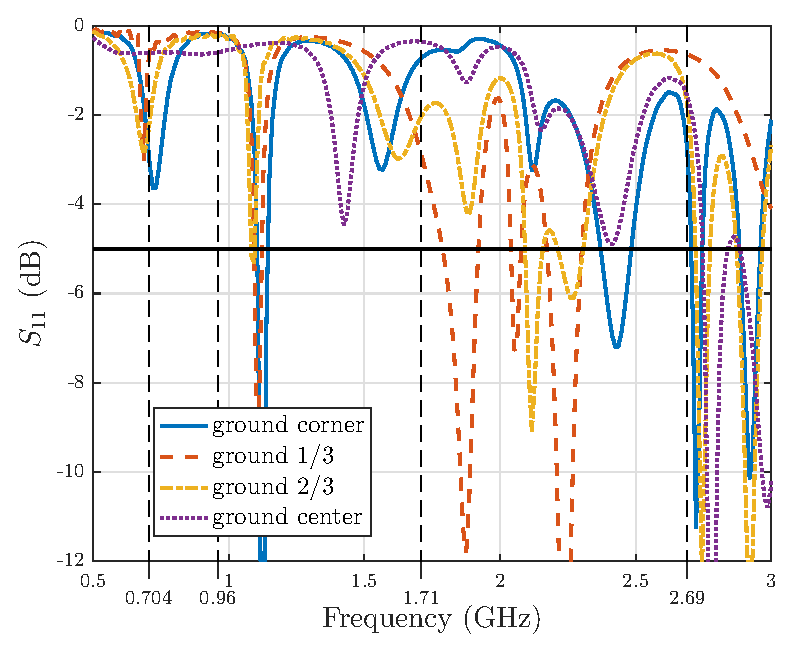
\includegraphics[width=\textwidth]{img/feed_pos_top_res.eps}
        \caption{Antenna located on the top of the phone.}
        \label{fig:feed_pos_top_res}
    \end{subfigure}
    \caption{The effect of the location of the feed.}
    \label{fig:feed_effect}
\end{figure}


\subsubsection{Position and shape of an antenna}
\label{sec:position_shape}

Positioning the antenna is as well worth testing. In this test, a $70\,\milli\meter$ long element is bent over a corner to form an L-shaped structure. The total length of this element is the same as was one option in testing the effect of length, to have comparability. The antenna is positioned in one corner of the phone in four different ways presented in Table \ref{tab:l_structures}. The lengths on each side are kept the same, and positioning is changed by rotating the element. The feed is placed in the corner of the ground plane, and is oriented along either the long or the short side. Figure \ref{fig:l_shape_model} illustrates the model. In this illustration feed is placed on the long side of the phone.

Results are presented in Figure \ref{fig:l_shape_res}. The nature of each curve is very similar, especially other structures but 1, that are almost identical below ca. $2.3\,\giga\hertz$. As these three structures have quite strong resonance above $1\,\giga\hertz$, the blue curve of structure 1 is showing promising wideband performance. Although the good band is just above the low band, where performance of each setup is very weak, this test shows that wide band matching might be achievable with L-shaped elements in the corners.

\begin{table}[H]
    \centering
    \caption{Antenna parameters used while testing L-shaped antenna structures.}
    \label{tab:l_structures}
    \begin{tabular}{|M{0.22\textwidth}|M{0.22\textwidth}|M{0.22\textwidth}|M{0.22\textwidth}|}
        \hline
        \textbf{Antenna structure} & \textbf{Antenna length on the long side ($l_1$)} & \textbf{Antenna length on the short side ($l_2$)} & \textbf{Feed orientation}\\
        \hline
         Structure A & $50\,\milli\meter$ & $20\,\milli\meter$ & On the long side\\
         \hline
         Structure B & $50\,\milli\meter$ & $20\,\milli\meter$ & On the short side\\
         \hline   
         Structure C & $20\,\milli\meter$ & $50\,\milli\meter$ & On the short side\\
         \hline
         Structure D & $20\,\milli\meter$ & $50\,\milli\meter$ & On the long side\\
         \hline
    \end{tabular}
\end{table}

\begin{figure}[H]
    \centering
    \begin{subfigure}[b]{0.49\textwidth}
        \includegraphics[width=\textwidth]{img/L_shape.eps}
        \caption{Model of L-shaped antenna.}
        \label{fig:l_shape_model}
    \end{subfigure}
    \begin{subfigure}[b]{0.49\textwidth}
        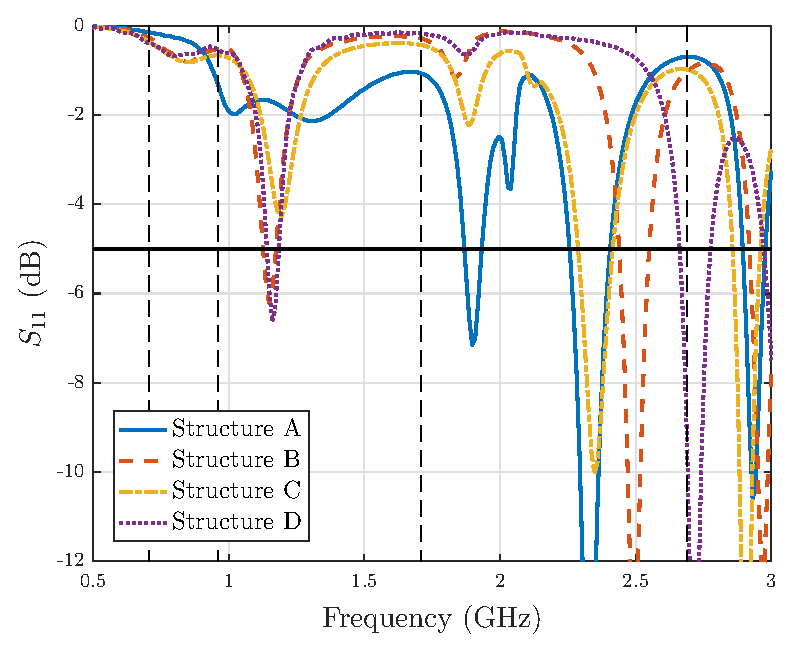
\includegraphics[width=\textwidth]{img/L_shape_res.eps}
        \caption{Results from simulations.}
        \label{fig:l_shape_res}
    \end{subfigure}
    \caption{Simulated L-shaped antennas.}
    \label{fig:l_shape}
\end{figure}

So far all investigated antennas have been either straight, rectangular sheets or L-shaped elements. Modifying the shape more might enable to excite different resonant modes. Figure \ref{fig:shape_models} shows six shapes of different complexity implemented on the top of the handset. All the tested structures are fed from the same corner of the ground plane. To make it clear, the antennas of shapes 4, 5, and 6 (\Cref{fig:shape4,fig:shape5,fig:shape6}, respectively) are $0.5\,\milli\meter$ apart from the cover.

\begin{figure}[H]
    \centering
    \begin{subfigure}[b]{0.49\textwidth}
        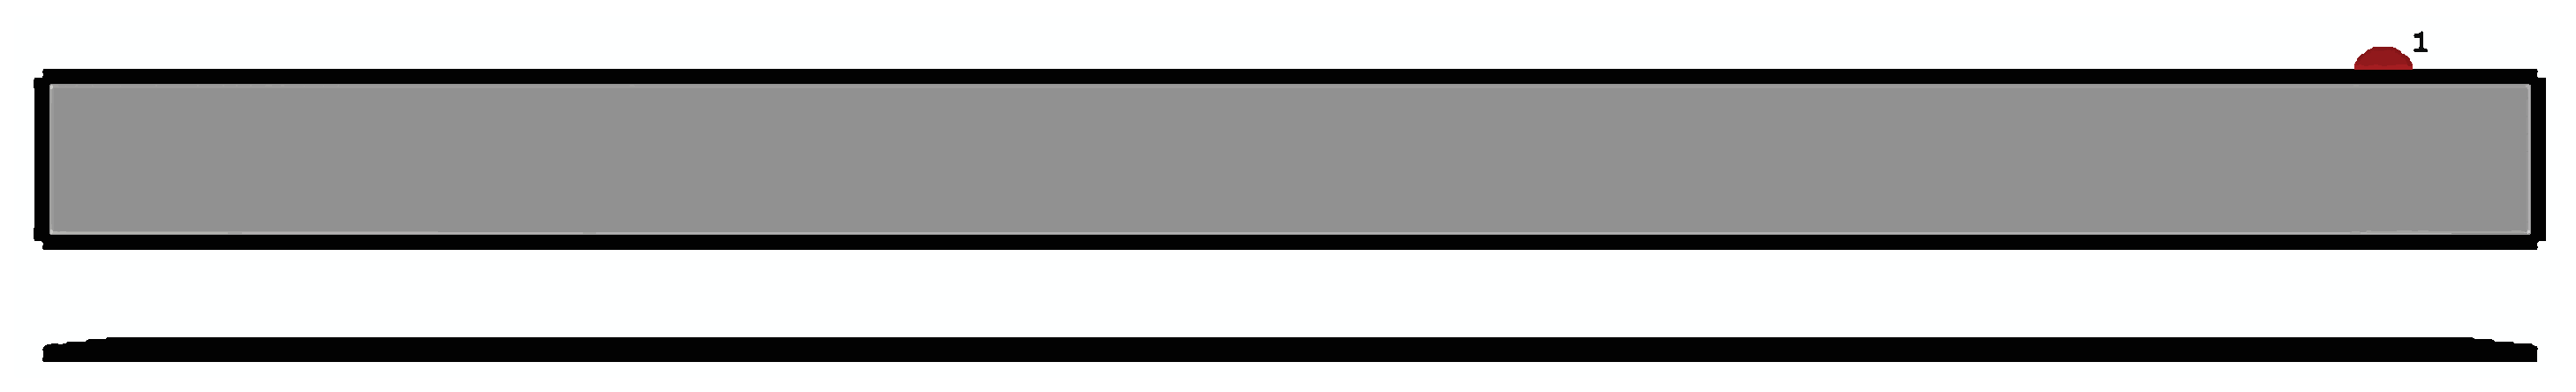
\includegraphics[width=\textwidth]{img/shape1.eps}
        \caption{Shape 1.}
        \label{fig:shape1}
    \end{subfigure}
    \begin{subfigure}[b]{0.49\textwidth}
        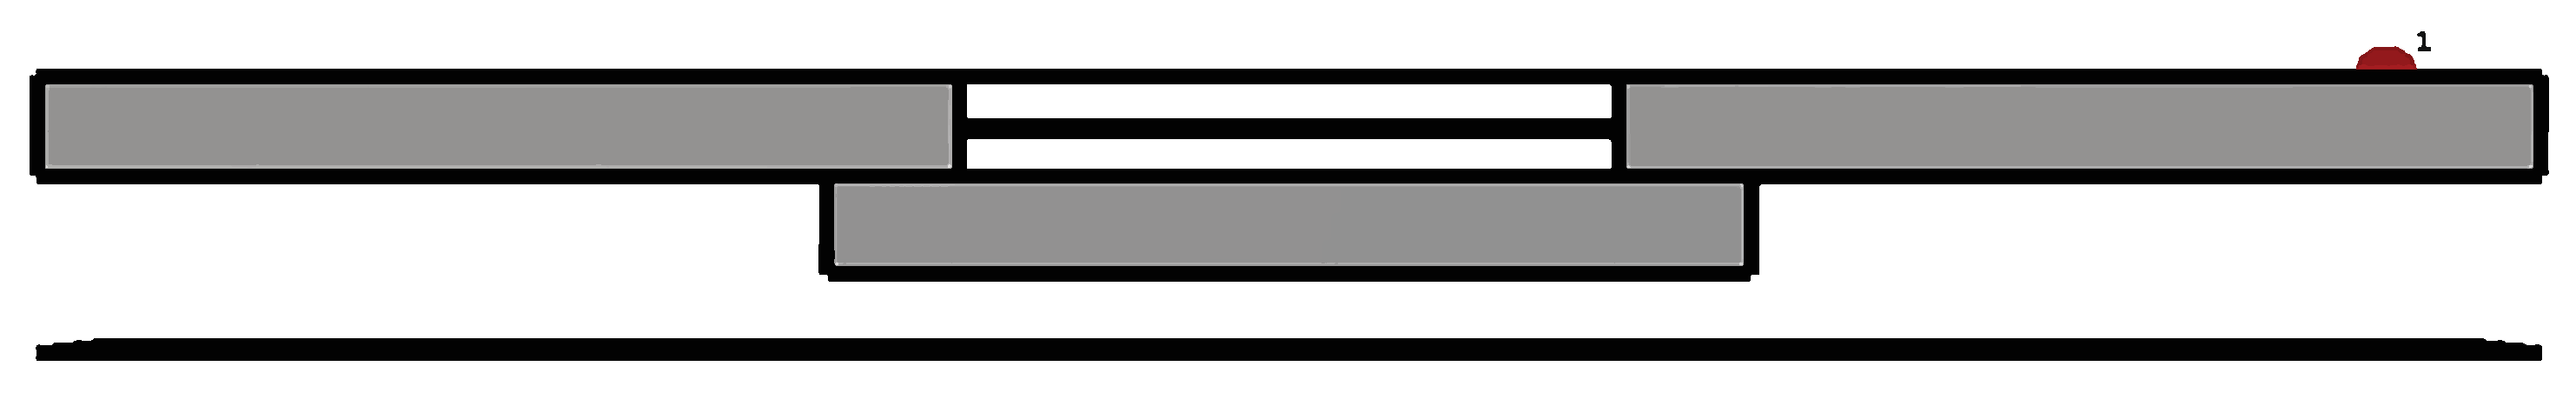
\includegraphics[width=\textwidth]{img/shape2.eps}
        \caption{Shape 2.}
        \label{fig:shape2}
    \end{subfigure}
    
    \begin{subfigure}[b]{0.49\textwidth}
        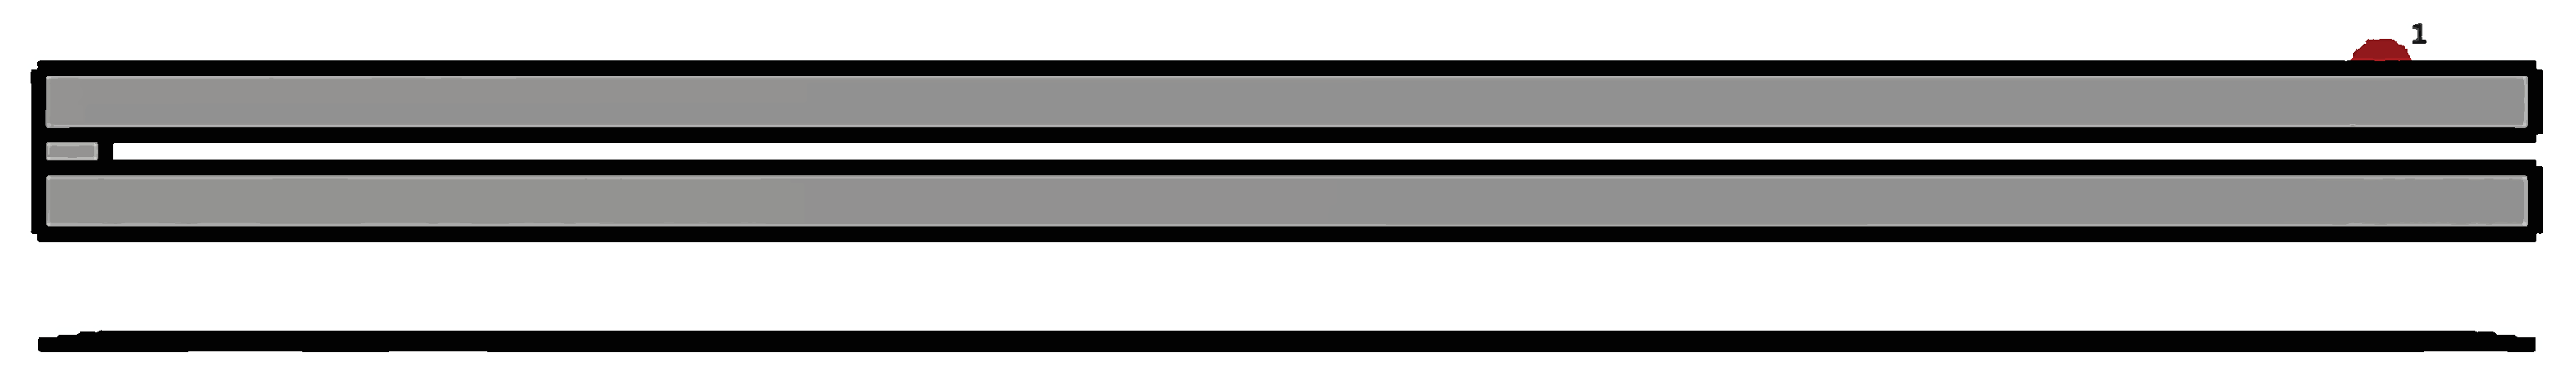
\includegraphics[width=\textwidth]{img/shape3.eps}
        \caption{Shape 3.}
        \label{fig:shape3}
    \end{subfigure}
    \begin{subfigure}[b]{0.49\textwidth}
        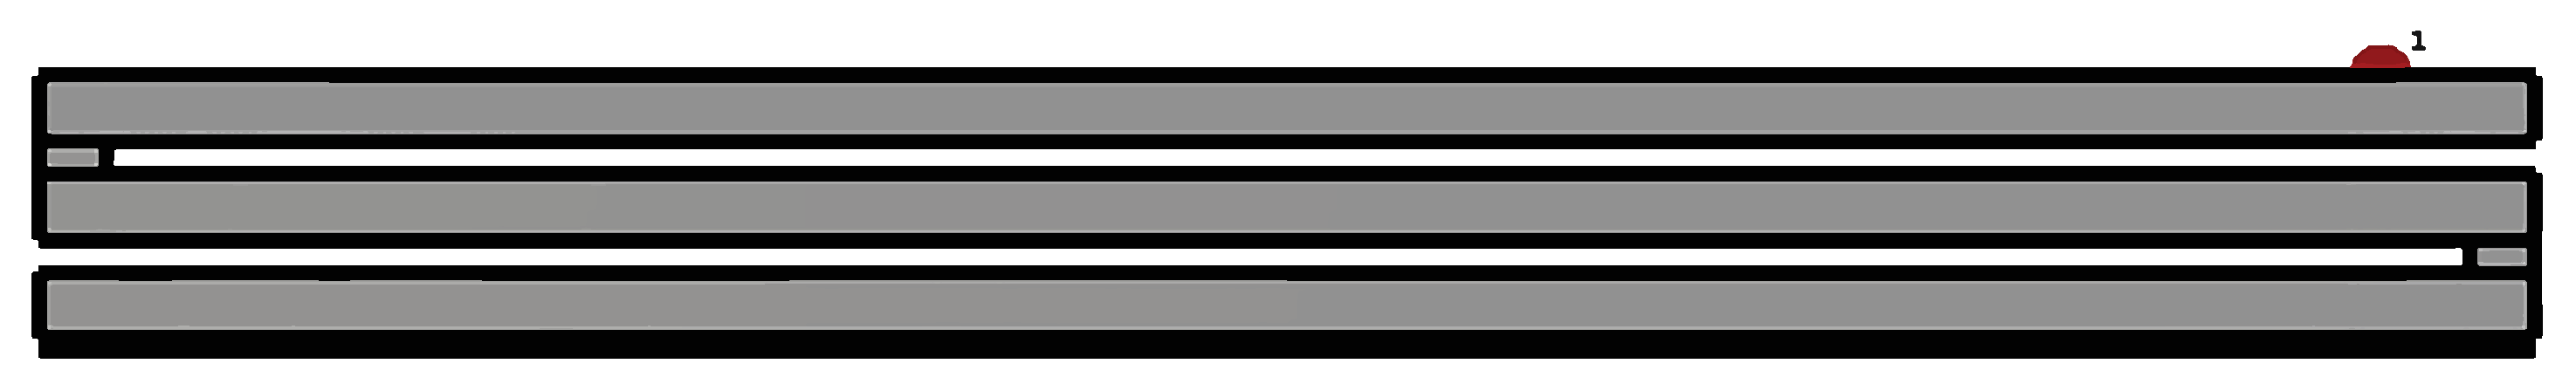
\includegraphics[width=\textwidth]{img/shape4.eps}
        \caption{Shape 4.}
        \label{fig:shape4}
    \end{subfigure}
    
    \begin{subfigure}[b]{0.49\textwidth}
        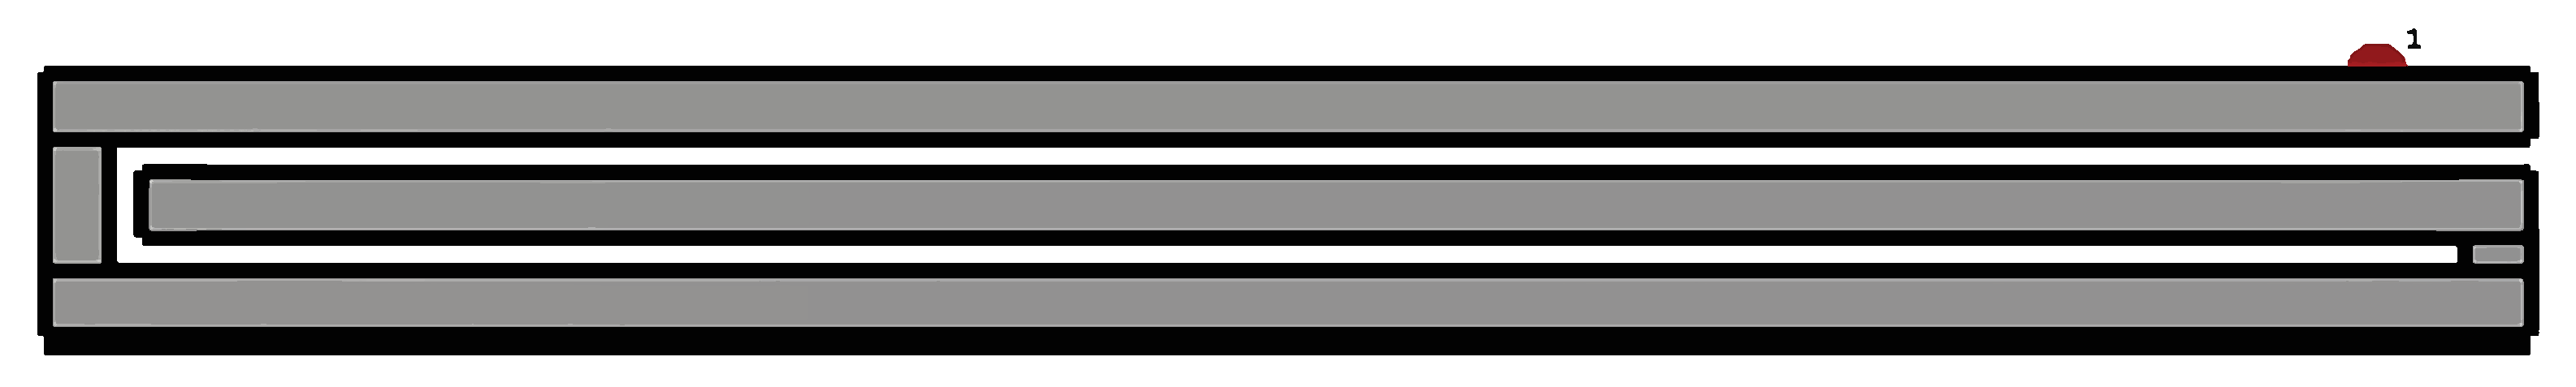
\includegraphics[width=\textwidth]{img/shape5.eps}
        \caption{Shape 5.}
        \label{fig:shape5}
    \end{subfigure}
    \begin{subfigure}[b]{0.49\textwidth}
        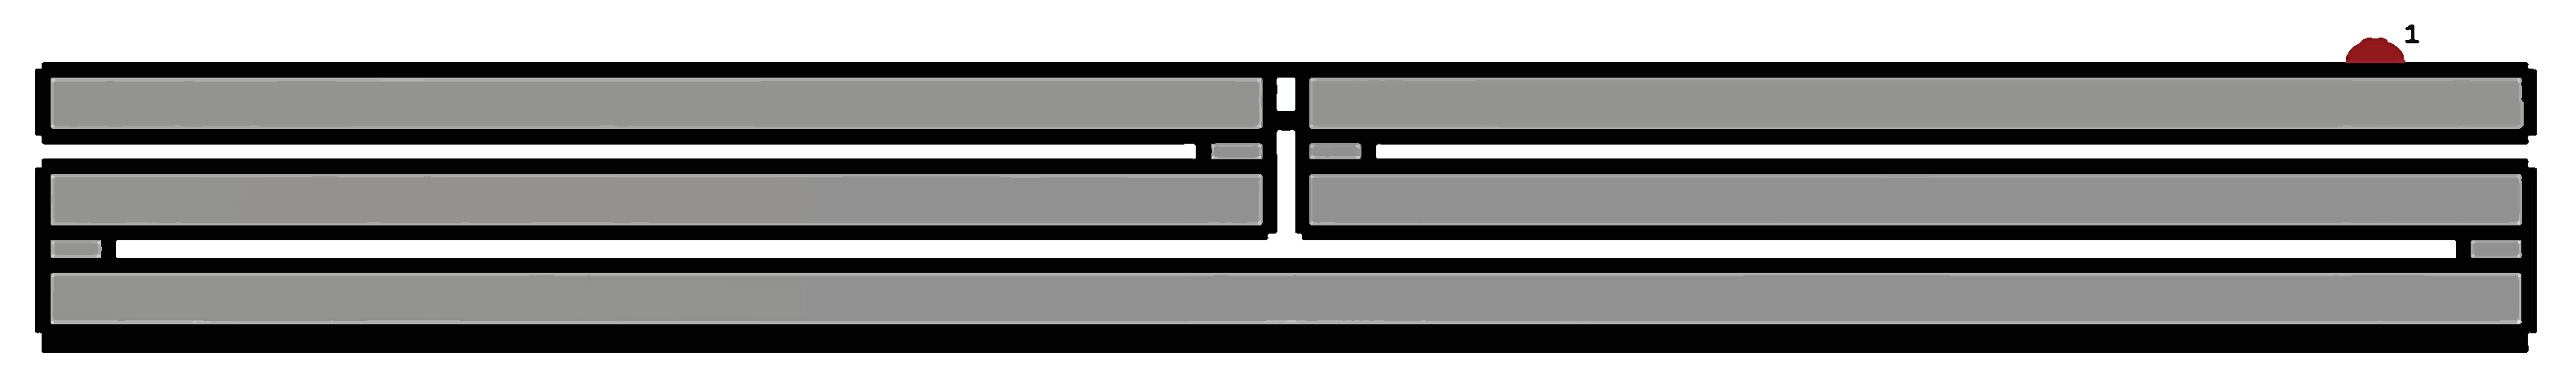
\includegraphics[width=\textwidth]{img/shape6.eps}
        \caption{Shape 6.}
        \label{fig:shape6}
    \end{subfigure}
    \caption{Different shapes for antenna located at the end of the phone.}
    \label{fig:shape_models}
\end{figure}

Results in Figure \ref{fig:shape} show that for the low band, shape 4 has the best matching and quite good bandwidth. The two most simple shapes, 1 and 2, produce almost identical results, and in the lowest frequencies they are somewhat wideband, though the matching level is poor. These simpler structures also operate better in the high band than other tested antennas.

\begin{figure}[H]
    \centering
    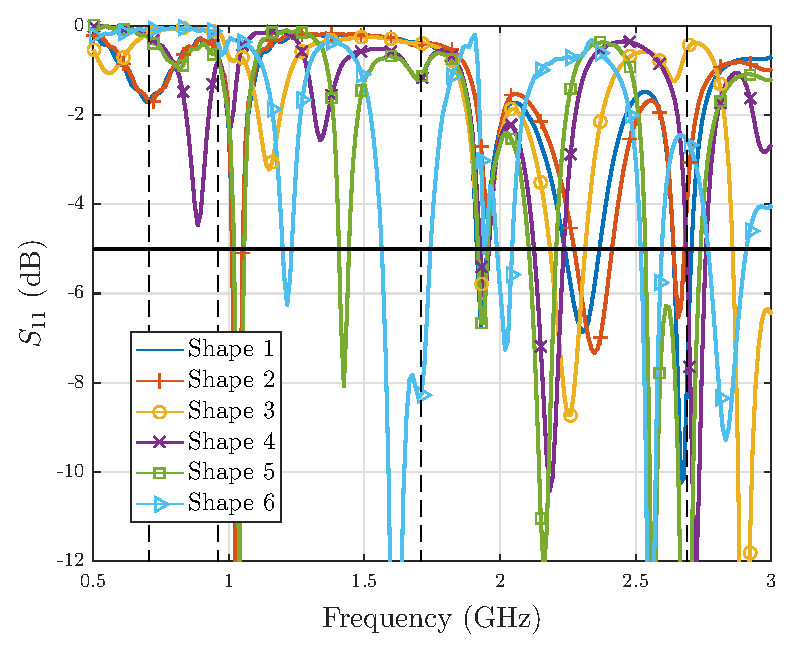
\includegraphics[width=0.5\textwidth]{img/shape.eps}
    \caption{Effect of different antenna shapes. Antennas are located at the end of a phone.}
    \label{fig:shape}
\end{figure}

As was shown in earlier Figure \ref{fig:metal_rim}, typical locations for antennas are the areas above and below the display of the phone. Therefore, an antenna element is placed in that area, illustrated in Figure \ref{fig:front_model}, and compared to a similar element located at the end of the phone, like shown in Figure \ref{fig:shape1}. Figure \ref{fig:front_res} shows that the difference between these two locations is minimal. The shapes of the responses are nearly identical in the low frequencies, and they follow the same pattern in the higher band. Matching levels at the low band are bad, but the bandwidth is quite wide. In the high band, the element on the front gives good matching on two sub-bands, and is promising in the rest of the band also.

\begin{figure}[H]
    \centering
    \begin{subfigure}[b]{0.49\textwidth}
        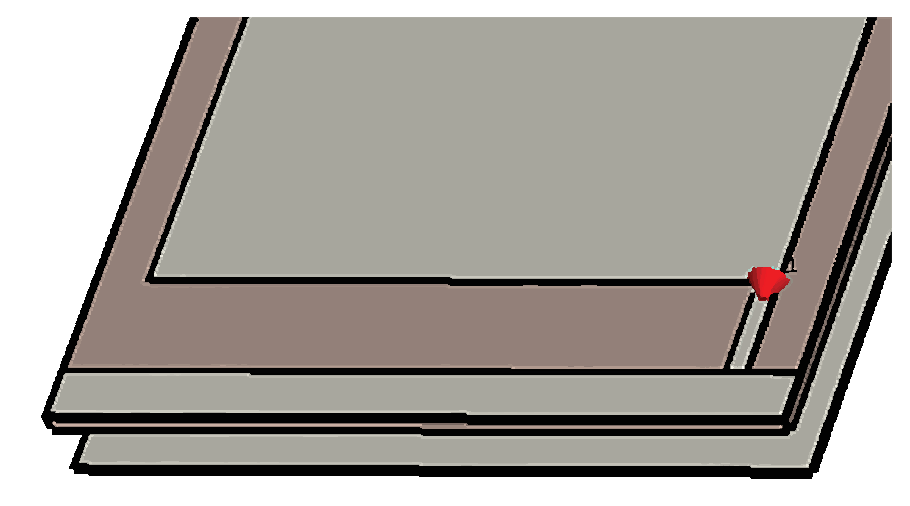
\includegraphics[width=\textwidth]{img/front.eps}
        \caption{Model of frontside antenna element.}
        \label{fig:front_model}
    \end{subfigure}
    \begin{subfigure}[b]{0.49\textwidth}
        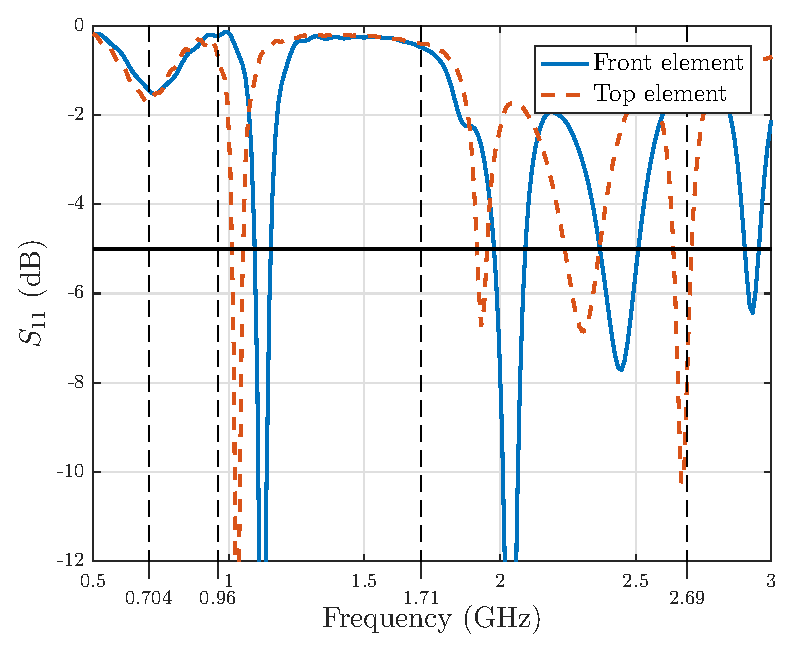
\includegraphics[width=\textwidth]{img/front_res.eps}
        \caption{Results from simulations.}
        \label{fig:front_res}
    \end{subfigure}
    \caption{Antenna element on the front side of the phone.}
    \label{fig:front_elem}
\end{figure}

In addition to straight elements, slots can be added to elements to introduce new wave modes. This test has the same antenna as presented in Figure \ref{fig:metal_cover}, with one or two slots on the sides. The first slot on the long side, at $20\,\milli\meter$ from the end, and second is on the short side at the same distance from the end of the element. Both slots are $2\,\milli\meter$ wide. The added slot is shown in Figure \ref{fig:slot}.
\begin{figure}[H]
    \centering
    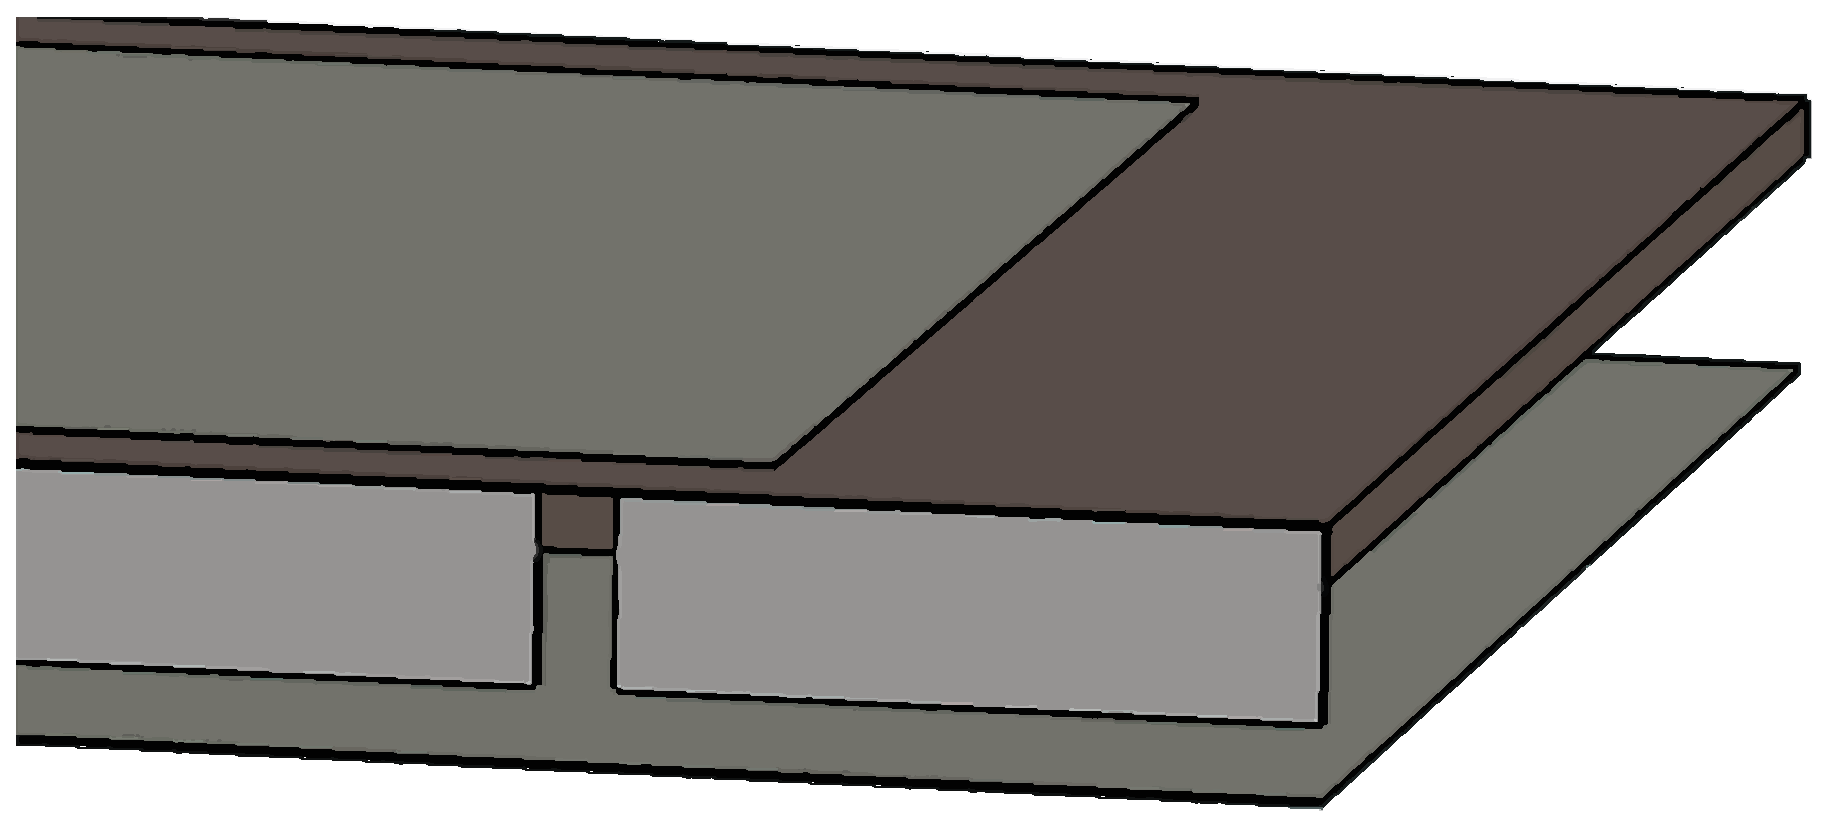
\includegraphics[width=0.5\textwidth]{img/slot.eps}
    \caption{Antenna element with slot in it.}
    \label{fig:slot}
\end{figure}

Adding one slot creates strong and very narrow peak resonance at the low band, as can be seen from Figure \ref{fig:slot_res}. The second slot gives slightly wider bandwidth, but decreases matching level compared to zero or one slot.

\begin{figure}[H]
    \centering
    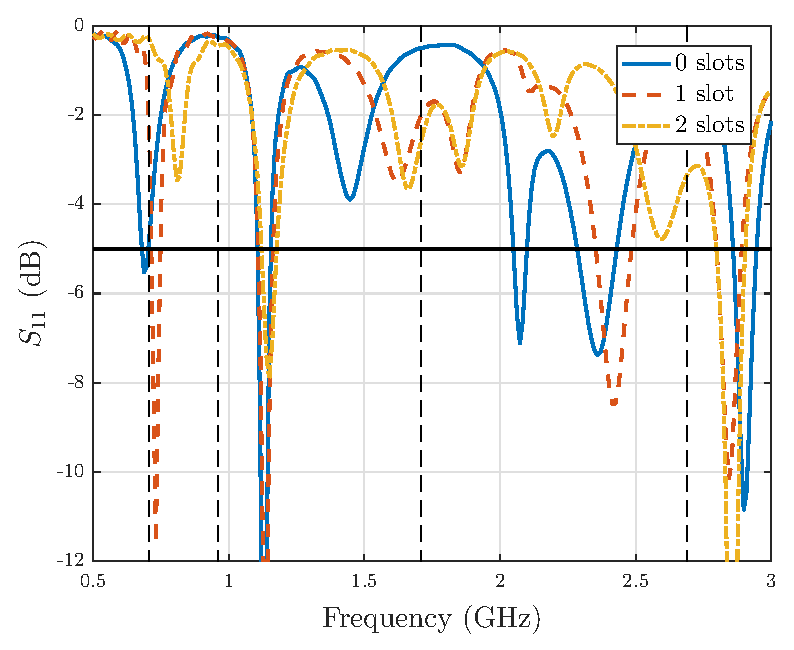
\includegraphics[width=0.5\textwidth]{img/slot_res.eps}
    \caption{Effect of slots in the antenna element.}
    \label{fig:slot_res}
\end{figure}

\subsubsection{Ground plane}
\label{sec:ground_plane}
Last thing to investigate is the effect of ground plane. So far phone's display has been used as a ground plane, but since the back cover is also large metallic plate, that could be used as well as a ground. The test setup is the same as was used to the effect of metal cover, shown in Figure \ref{fig:metal_cover}. Only feed is moved between the iterations. Figure \ref{fig:ground_plane} shows the impact. When feed is moved to locate between the back cover and the antenna element, the response is slightly more resonating, but has wider bandwidths and generally better matching levels. One possible explanation for this behavior might rely on the sizes of the two planes. When display is used as a ground plane, the larger back cover interacts with the EM-fields stronger and therefore is more harmful for the antennas. If feed is grounded to the back cover, then the disturbing element is smaller and negative effects are not as strong.

\begin{figure}[H]
    \centering
    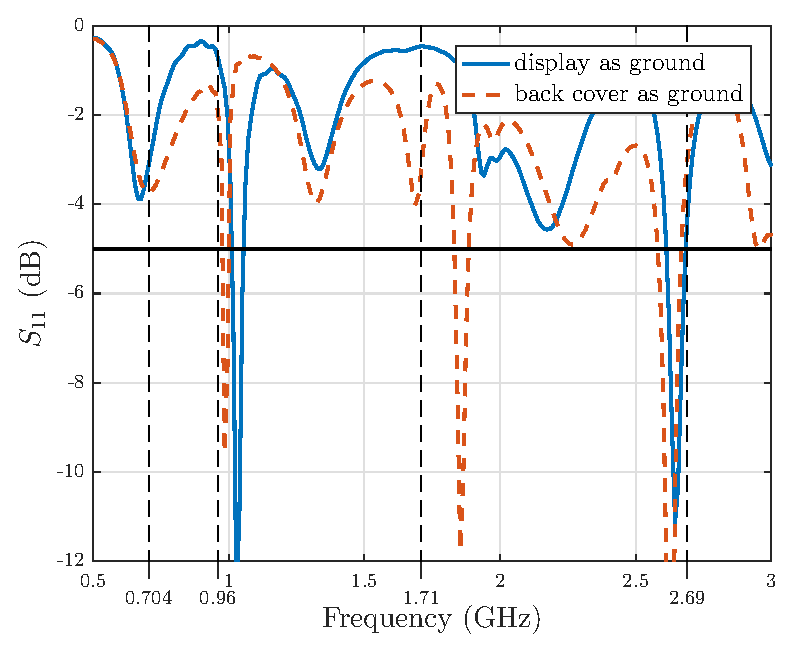
\includegraphics[width=0.5\textwidth]{img/ground_vs_display.eps}
    \caption{Effect of using display or back cover as ground plane.}
    \label{fig:ground_plane}
\end{figure}

\subsubsection{Summary of the pre-study}
\label{sec:pre_study_summary}
The conclusions made from all these presented simulation results are collected and summarized in Table \ref{tab:dimension_summary} below. 

\begin{table}[H]
    \centering
    \caption{Summary of how changing dimensions affect antenna's performance.}
    \label{tab:dimension_summary}
    \begin{tabular}{|p{0.28\textwidth}|p{0.33\textwidth}|p{0.33\textwidth}|}
        \hline
        \textbf{Changed parameter} & \textbf{Impact at LB} & \textbf{Impact at HB}\\
        \hline
        Element length on the side of the phone & Resonances are outside the band. & Shorter elements operate better.\\
        \hline
        Element length at the end of the phone & Longer elements operate better. & Smaller elements operate slightly better.\\
        \hline
        Element on the front side of the phone & No major difference. & Matching levels are slightly improved.\\
        \hline
        Element width & Wider element slightly increases bandwidth. & Wider element slightly increases bandwidth.\\
        \hline
        Location of the feed & Feed close to a corner of the display gives wider band. & No major difference if feed is at the long side. At the end its better to closer to the center of the ground.\\
        \hline
        Ground plane & Improved matching levels & More resonance frequencies and better matching levels.\\
        \hline
        Shape of the element & Simpler is better. & L-shape resonates less than more complex shapes.\\
        \hline
        Slots & Slots create narrow resonances. & Matching levels decrease with slots.\\
        \hline
    \end{tabular}
\end{table} 

\clearpage

%\section{Simulaatiot}
\section{Antenna simulations}
\label{sec:simulations}
This section contains the majority of the work for this thesis. The design problem is approached with two models of various complexity, and the antenna structure is developed in an organized way. Different subsections explain and present the results of different phases of the simulation process. Finally, all pieces are put together and the complete structure is formed.


\subsection{Conceptualizing the main antenna}
\label{sec:conceptualizing}
After the pre-studies, the actual concept for the main antenna is based on the design introduced in \cite{kimmo}. The findings from the pre-study also support the chosen approach. The main antenna should be located mainly on the short side of the phone and construct of simple shapes. Its elements should be rather short and they can be bended over the corner of the phone. Also, it is noticed that slots might improve bandwidth, and thus, could be used to cover both defined frequency sets. 

So, the main antenna is decided to consist of three elements. Two of them are L-shaped strips bending over the corners of the phone. The third element is a U-shaped sheet on the frontside of the phone, above the display. Back cover is used as a ground plane since it is earlier found to be better choice than the display. At first, this structure is single-fed, and the feed is connected between the U-shaped element and the ground plane. Figure \ref{fig:main_concept} shows the structure of this concept, and Figure \ref{fig:main_location} gives a better view of the location of the antenna.

\begin{figure}[H]
    \centering
    \begin{subfigure}[b]{0.49\textwidth}
        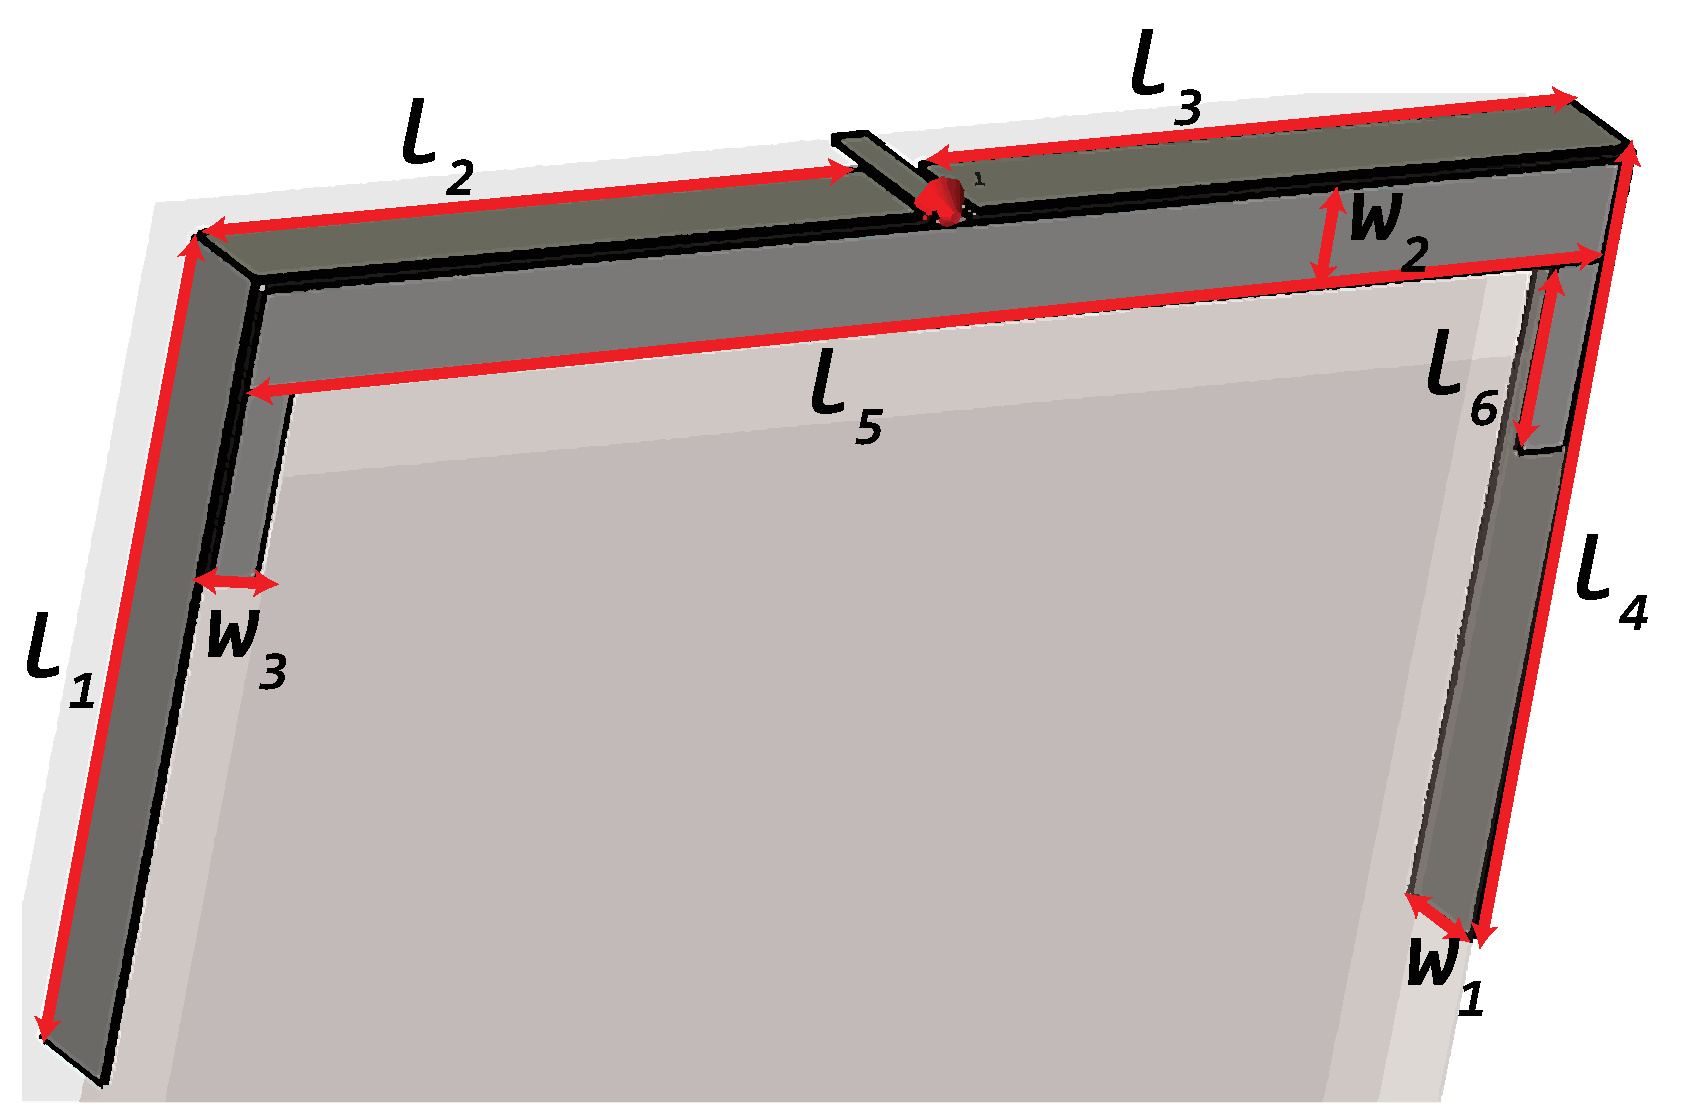
\includegraphics[width=\textwidth]{img/main_concept.eps}
        \caption{Structure.}
        \label{fig:main_concept}
    \end{subfigure}
    \begin{subfigure}[b]{0.49\textwidth}
        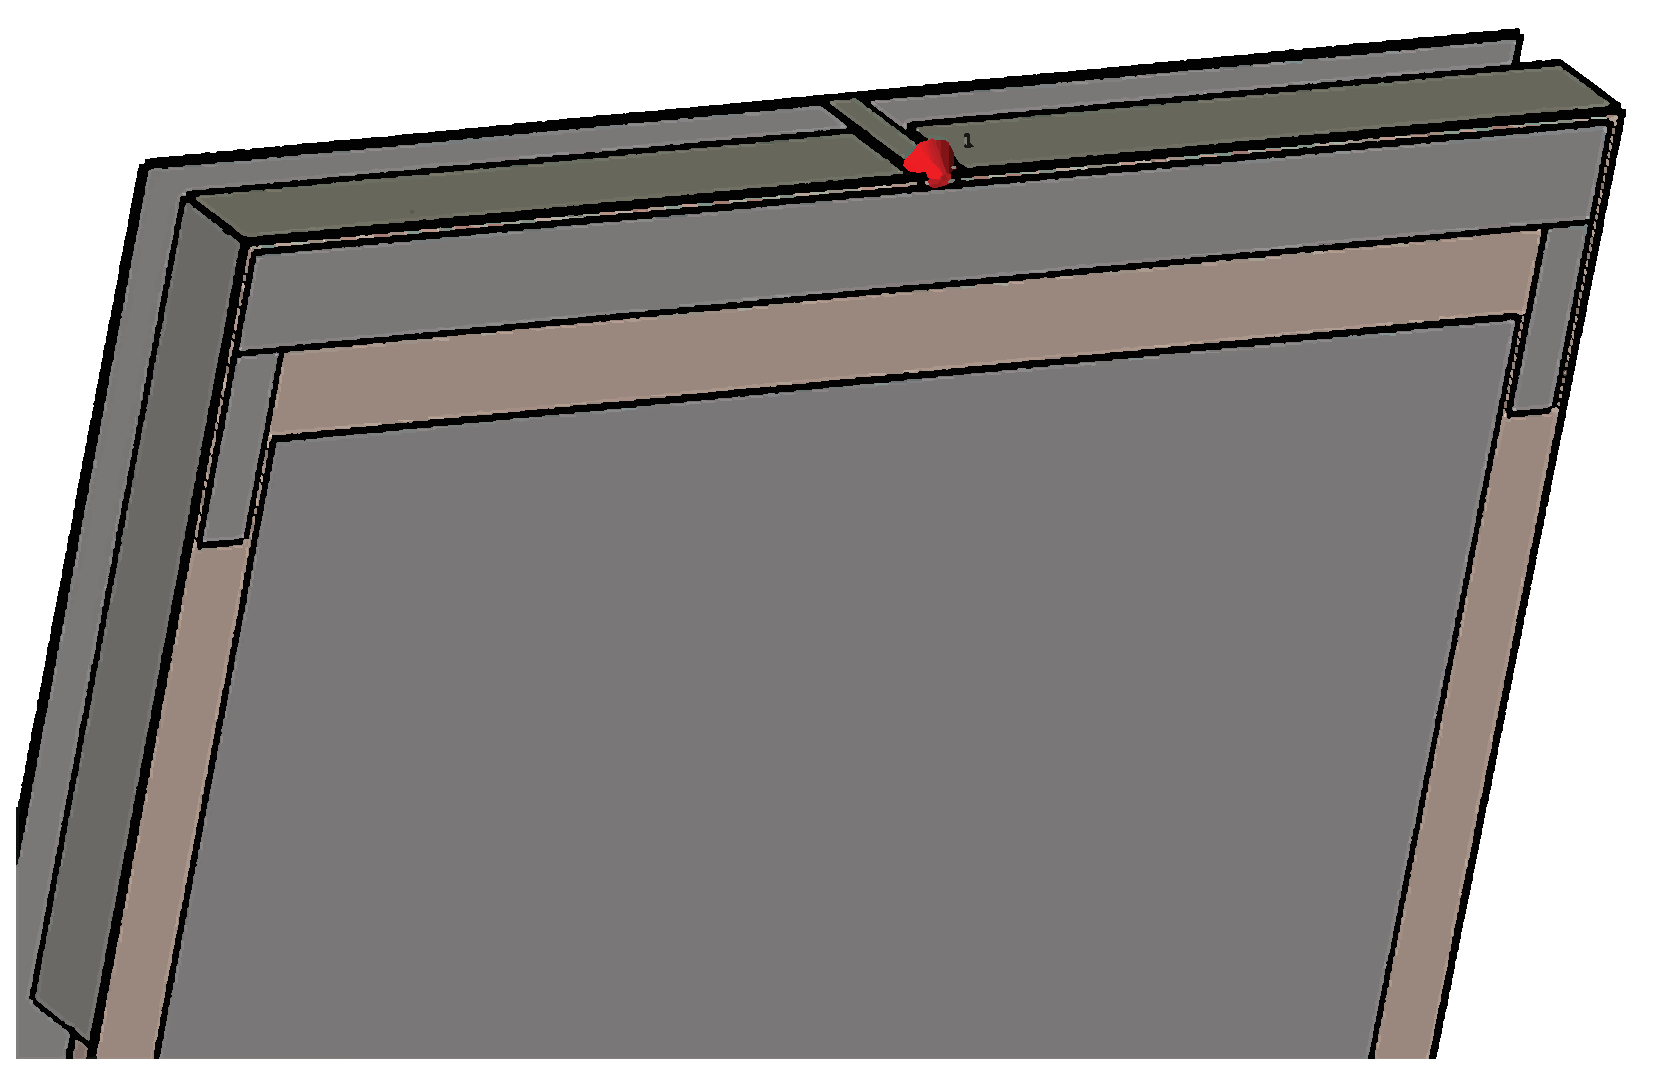
\includegraphics[width=\textwidth]{img/main_location.eps}
        \caption{Location.}
        \label{fig:main_location}
    \end{subfigure}
    \caption{The concept for the main antenna.}
    \label{fig:main_antenna1}
\end{figure}

The underlying idea of this structure is to have a strong mutual coupling between the three antenna elements, which would hopefully improve the operational bandwidth of the system. The elements are placed very close to each other to have better coupling effect. The gap between the U-shaped and the L-shaped elements is only $0.5\,\milli\meter$. The same gap width is also used between the barbs of the U-antenna and the display, and to separate the L-elements from the feed pin.


\subsubsection{Initial concept}
\label{sec:initial_concept}
The concept is improved and modified further via a number of simulation iterations. Between the different simulation rounds, the structures and dimensions are modified the same way as it is done in the preliminary study. The main values of interest are highlighted in Figure \ref{fig:main_concept}, and their initial values can be seen from Table \ref{tab:initial_concept}. Besides these parameters, also the location of the feed and the different gaps between the elements are tested. 
\begin{table}[H]
    \centering
    \caption{Initial values for the main antenna concept.}
    \label{tab:initial_concept}
    \begin{tabular}{|c|c|}
        \hline
        \textbf{Dimension} & \textbf{Value [$\milli\meter$]} \\
        \hline
        $l_1$ & 40\\
        \hline
        $l_2$ & 36.5\\
        \hline
        $l_3$ & 36.5\\
        \hline
        $l_4$ & 40\\
        \hline
        $l_5$ & 75\\
        \hline
        $l_6$ & 9.5\\
        \hline
        $w_1$ & 5\\
        \hline
        $w_2$ & 5\\
        \hline
        $w_3$ & 2.55\\
        \hline
    \end{tabular}
\end{table}

Already the first simulation in Figure \ref{fig:concept_ini} shows very promising results. Shape of the response in the low band is exactly what is desired: wide and smooth. However, the results are not all positive. The matching level in the low band is only about $-2\,\db$, and the high band is terrible. The first conclusion of this result is that either symmetric structure is not optimal or the dimensions of the different parts are not what they are supposed to be.
\begin{figure}[H]
    \centering
    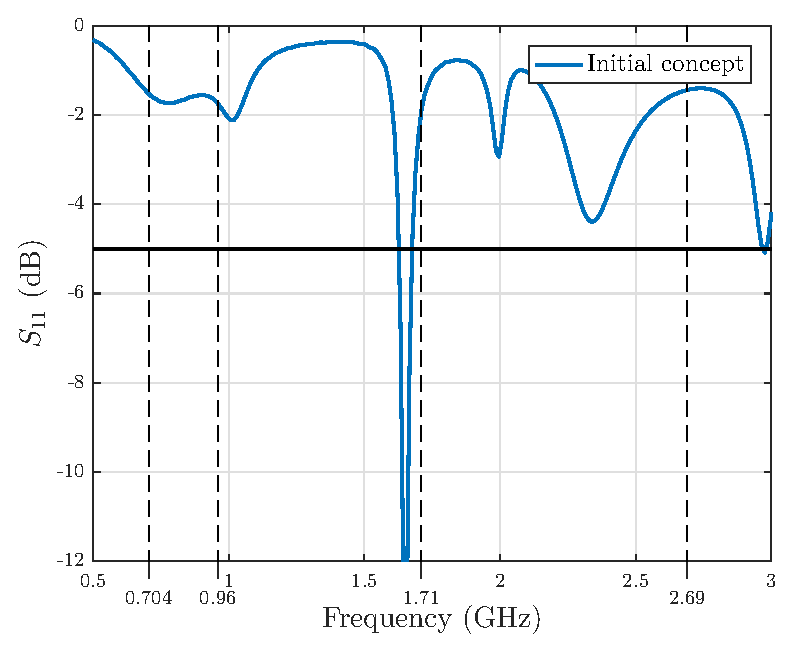
\includegraphics[width=0.5\textwidth]{img/concept_ini.eps}
    \caption{The simulation result for the initial concept.}
    \label{fig:concept_ini}
\end{figure}


\subsubsection{Iteration of dimensions}
\label{sec:dimension iteration}
The structure is first modified by changing the dimensional parameters. For now, the system is still kept symmetric to preserve simplicity. The changed dimensions are the lengths of the metal sheets beside the display ($l_6$), lengths of the antennas on the sides of the phone ($l_1$, $l_4$) and the width of all the side antennas ($w_1$). All these parameters are tested separately by the same principles that are used in the preliminary study, but in more detail. As the observations are similar to the ones in the preliminary study, only the best results are reported. Table \ref{tab:concept2} lists the best values for these parameters found in the three cases. Cases A, B, and C refer to changing $l_6$, $l_1$ and $l_4$, or $w_1$, respectively. 
\begin{table}[H]
    \centering
    \caption{Tested dimensions. All values are in millimeters.}
    \label{tab:concept2}
    \begin{tabular}{|c|c|c|c|c|}
        \hline
        \textbf{Dimension} & \textbf{Initial} & \textbf{Case A} & \textbf{Case B} & \textbf{Case C}\\
        \hline
        $l_1$ & 40 & 40 & 26 & 26\\
        \hline
        $l_4$ & 40 & 40 & 26 & 26\\
        \hline
        $l_6$ & 9.5 & 2.5 & 2.5 & 2.5\\
        \hline
        $w_1$ & 5 & 5 & 5 & 4\\
        \hline
    \end{tabular}
\end{table}

The values of tested dimensions range from both larger than the initial value to smaller than that. Table \ref{tab:concept2} above shows that the best values are smaller than the initial one for all parameters. The results especially for $l_1$, $l_4$, and $l_6$ agree with the findings from the pre-study: better low band is achieved with smaller element on the side. $w_1$ however is smaller than the initial width but provides better results, even though the pre-study shows the opposite. In this case, as it is in the pre-study, the variations in the matching level between the different widths are marginal, but the chosen $4\,\milli\meter$ provided the smoothest response in the low band.

Figure \ref{fig:concept2} shows the best results of the tested three cases compared with the initial situation. Each modification have improved system's performance in the low band. Although the focus is still in the low band, the high band should not be forgotten. In that area, the overall performance has not improved as the structure is modified. 
\begin{figure}[H]
    \vspace{-5pt}
    \centering
    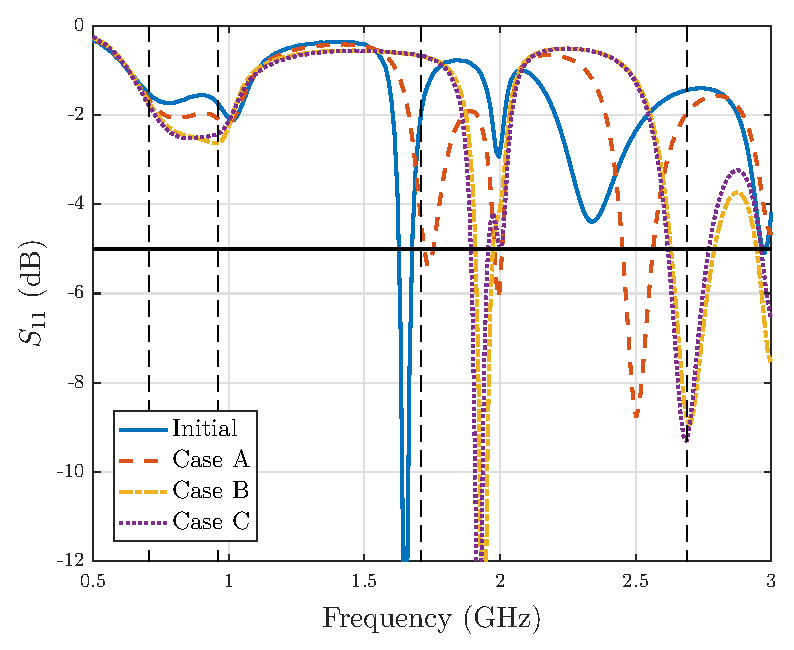
\includegraphics[width=0.5\textwidth]{img/concept2.eps}
    \caption{The best results from the three test cases.}
    \label{fig:concept2}
\end{figure}

Since the response of Case C in the low band is wide and below $-2\,\db$, a matching circuit is generated for it with Optenni Lab. The program is set to generate a three-element circuit for either only low band or both bands aiming for the defined $-5\,\db$ matching level. Figure \ref{fig:concept2_match} presents the results. The desired matching level is reached in neither of the two settings. When only the low band is matched, a decent level of $-4\,\db$ on average is obtained. Adding the requirement for the high band does not create much difference to the situation without any matching circuits. 
\begin{figure}[H]
    \centering
    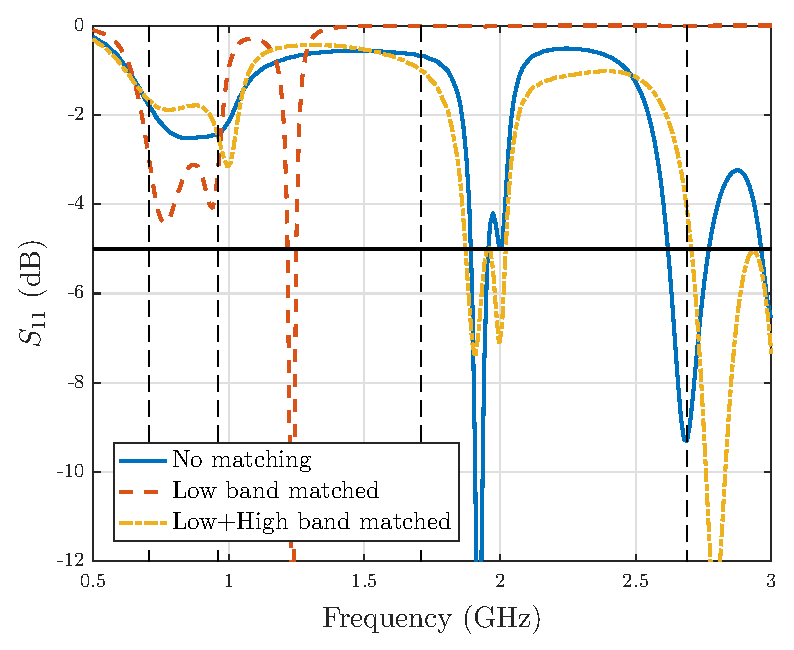
\includegraphics[width=0.5\textwidth]{img/concept2_match.eps}
    \caption{The simulation results of Case C with different matching circuits.}
    \label{fig:concept2_match}
    \vspace{-10pt}
\end{figure}

Since a suitable matching network could not be found for this structure, it means that the antennas should be modified more. One option would be to create two parallel matching circuits, one for the low band and the other for the high band. This however would increase the complexity of the system, which is undesired. Other possible solution could be modifying the antenna structures to be asymmetric, which is the preferable choice of the two options.


\subsubsection{Asymmetric structures}
\label{sec:asymmetric_structures}
Asymmetric structures are tested with four different cases. Case D has an offset in the location of the feed, which causes the top-parts of the L-shaped elements to have different lengths. In Case E, the antenna parts on the sides of the phone are of different length. For Case F, the feed is transferred to the corner of an L-shaped element and in Case G, the feed is offsetted from the previous location.

Again, only the best structures are presented of each case. Table \ref{tab:concept3} shows the changes in dimensions done in Cases D and E. In the best scenario of Case D the amount of offset is $3.5\,\milli\meter$ to the left, and in Case G $5\,\milli\meter$ to the right. 
\begin{table}[H]
    \vspace{-6pt}
    \centering
    \caption{Dimensional changes made to create asymmetry. All values are in millimeters.}
    \label{tab:concept3}
    \vspace{-5pt}
    \begin{tabular}{|c|c|c|}
        \hline
        \textbf{Dimension} & \textbf{Case D} & \textbf{Case E}\\
        \hline
        $l_1$ & 26 & 20 \\
        \hline
        $l_2$ & 33 & 33\\
        \hline
        $l_3$ & 40 & 40\\
        \hline
        $l_4$ & 26 & 30\\
        \hline
    \end{tabular}
\end{table}

Figure \ref{fig:concept_offsets} illustrates the structural changes of Cases D-G. The feed offset introduced in Case D is seen in Figure \ref{fig:concept3_u_offset}. The red dashed line shows the original location of the feed, in the middle of the side frame. Also the changes in the lengths of the L-elements (Case E) can be seen. Figure \ref{fig:concept_l_feed} shows the feeding structure of Case G, and the red dashed area points out the feed position in Case F.

\begin{figure}[H]
    \centering
    \begin{subfigure}[b]{0.49\textwidth}
        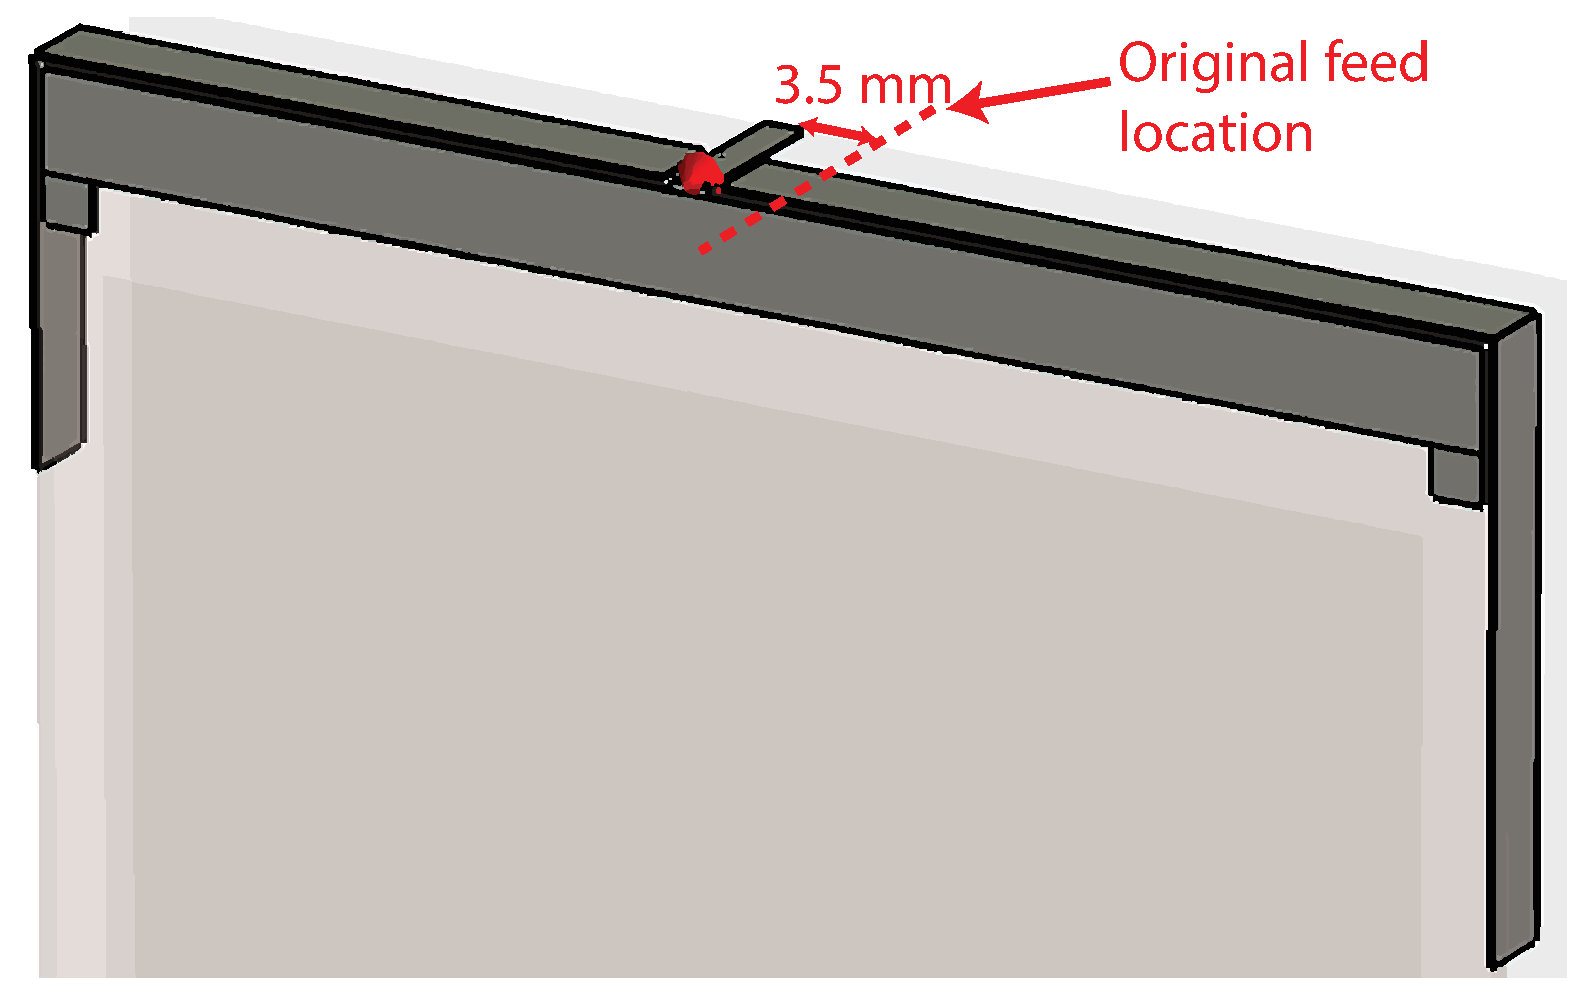
\includegraphics[width=\textwidth]{img/concept3_u_offset.eps}
        \caption{The feed offset in the U-shaped element.}
        \label{fig:concept3_u_offset}
    \end{subfigure}
    \begin{subfigure}[b]{0.49\textwidth}
        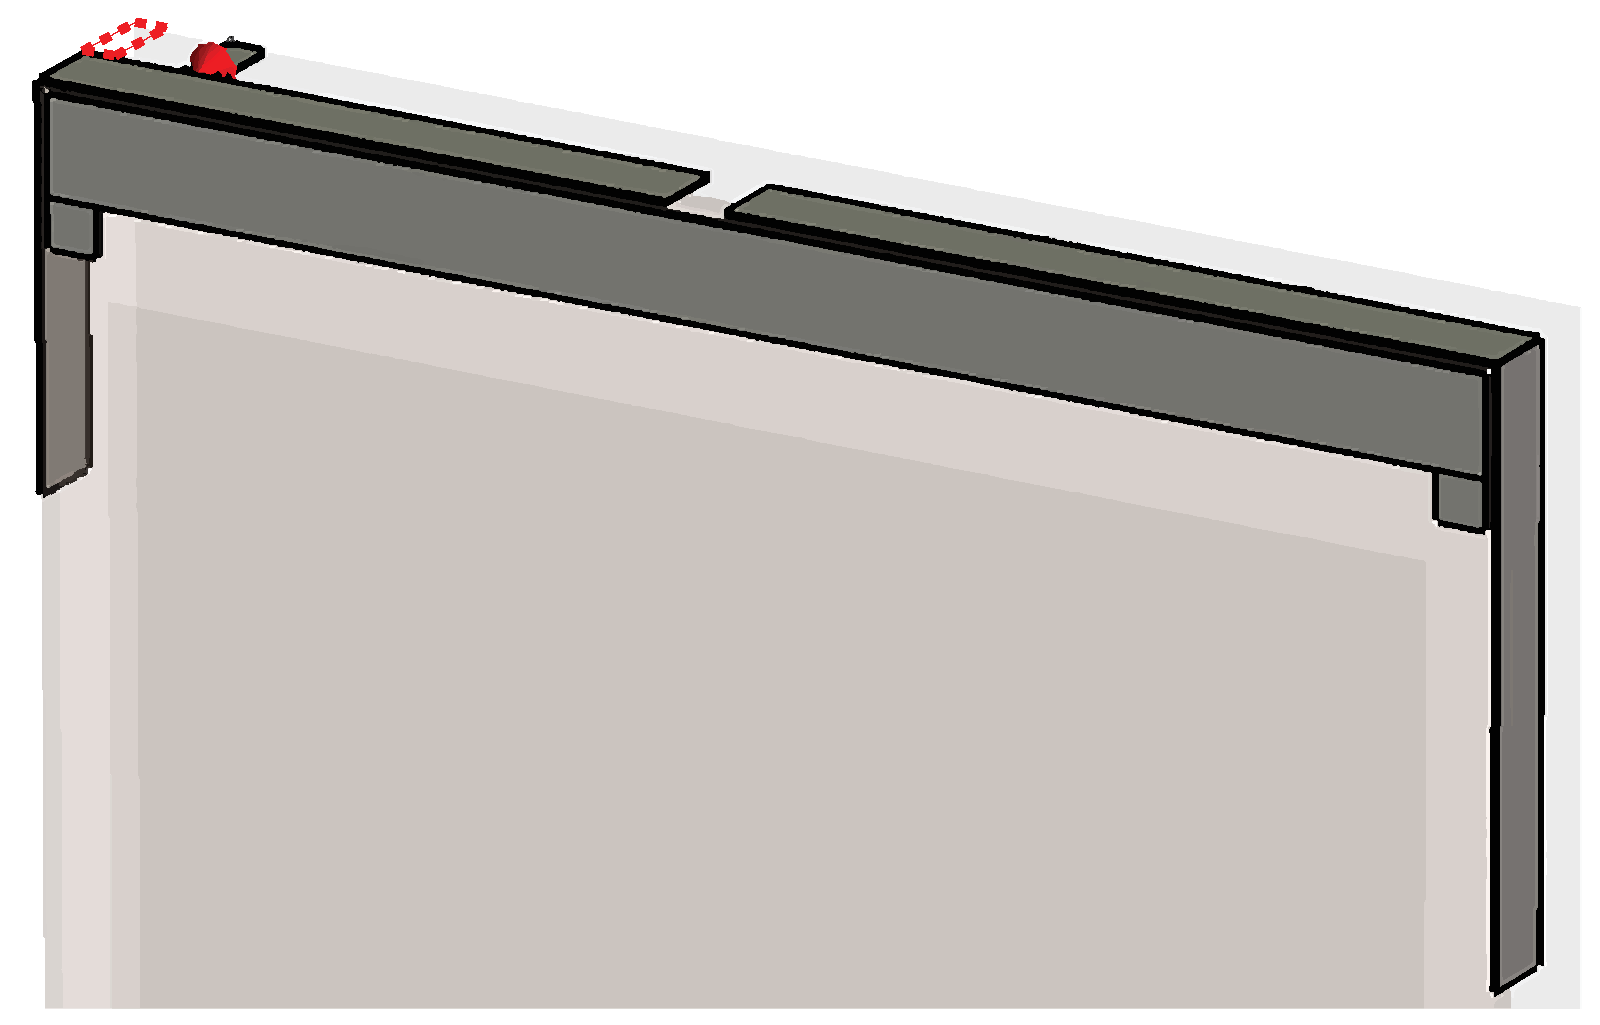
\includegraphics[width=\textwidth]{img/concept_l_feed.eps}
        \caption{Feed in the L-shaped element.}
        \label{fig:concept_l_feed}
    \end{subfigure}
    \caption{The changes in antenna structure in Cases D-G.}
    \label{fig:concept_offsets}
\end{figure}

Similarly to the cases with symmetric structures, the performance of the antenna system improved as the test cases proceeded, like Figure \ref{fig:concept3} represents. Matching in the low band is still wide and levels have increased. Besides that, also upper band is showing major enhancements, especially in Cases F and G. Matching levels are fair at the whole band. The only drawback is that the response in the high band resonates a lot, which might be a problem when generating matching circuits.
\begin{figure}[H]
    \centering
    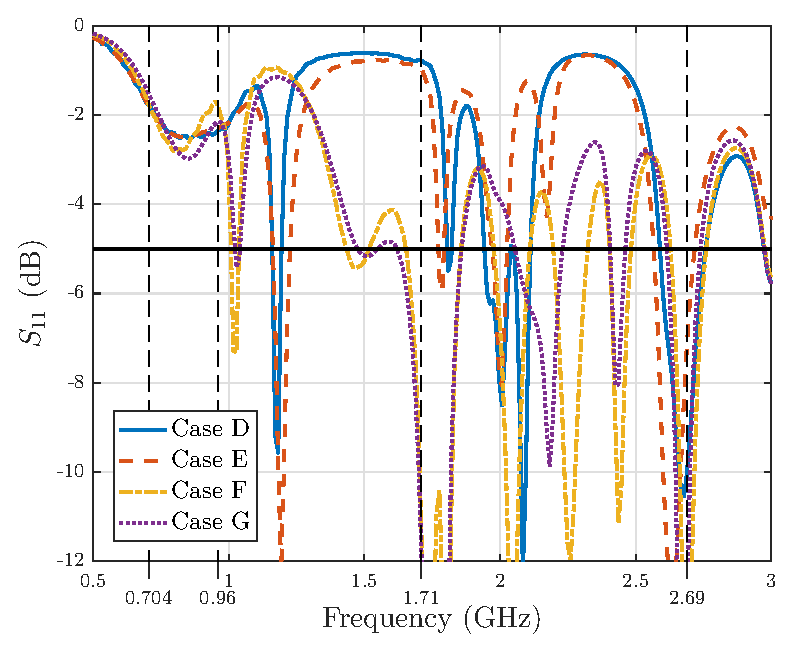
\includegraphics[width=0.5\textwidth]{img/concept3.eps}
    \caption{The best results from different asymmetric structures.}
    \label{fig:concept3}
\end{figure}

A matching network is generated also for the antenna of Case G. Optenni Lab is set to construct matching circuits for either low band, high band, or both bands with the target level of $-5\,\db$. Each topology has three components. Responses can be seen from Figure \ref{fig:concept3_match}. Surprisingly, the responses are more or less identical, even with the one without matching circuits. In the low band, a little more bandwidth is obtained when the antenna is matched, however, the matching level is still much worse than the target. In the high band, all topologies provide better matching but the target level is not completely reached. One curious observation is that Optenni Lab resulted the same topology for matching only low band or both bands. It can be concluded that the environment is very challenging for designing low band antennas, and moreover, matching them.
\begin{figure}[H]
    \centering
    \includegraphics[width=0.5\textwidth]{img/concept3_match.eps}
    \caption{Impedance matching results for Case G with different matching topologies.}
    \label{fig:concept3_match}
\end{figure}

Accordingly, the antenna concept requires some asymmetry in the structure, and also is quite precise of its dimensions. Next, the element above the display is modified. Case H changes the gap between the U-shaped element and the top of the phone from $0.5\,\milli\meter$ to $1\,\milli\meter$, which is seen as $w_2$ decreasing to $4.5\,\milli\meter$. The most radical modification is seen in Case I, where the barbs of the U-shaped element are removed, and only a straight metallic sheet is left (later referred as an I-shaped element). Figure \ref{fig:concept_i_shape} shows the updated structure.
\begin{figure}[H]
    \centering
    \includegraphics[width=0.5\textwidth]{img/concept_i_shape.eps}
    \caption{Antenna structure with the larger gap between elements from Case H and I-element from Case I.}
    \label{fig:concept_i_shape}
\end{figure}

Figure \ref{fig:concept4} shows the best results of Cases H and I, compared to Case G of the previous round of tests. Transforming the U-element to an I-element is a good change. Even though the low band is a little off the required frequencies, achieved bandwidth is wider and smoother than in any test so far. Progress has also happened in the high band, where the response is not that resonating anymore. Instead, the overall shape is not as resonating as before, and matching levels are mainly better.
\begin{figure}[H]
    \centering
    \includegraphics[width=0.5\textwidth]{img/concept4.eps}
    \caption{Simulation results from Cases H and I.}
    \label{fig:concept4}
    \vspace{-12pt}
\end{figure}

\subsubsection{Antenna structure with multiple feeds}
\label{sec:multiple_feeds}
The conceptualizing phase is concluded by testing a structure with multiple feeds. So far, all structures in the pre-study and conceptualizing tests have had one only feeding port. As this now studied structure consists of three separate but closely located elements, adding feeds to each of them is simple. This kind of system would result a few advantages. First, the mutual coupling effect might be stronger and enable larger achievable bandwidth. Second, matching the elements may be simpler since each feeding port can be assigned with its own set of frequencies. However, this will increase the complexity of the whole system.

Figure \ref{fig:concept_3feeds_struct} shows the modified structure for this test. Now the system has actually three antennas, named Element 1, 2, and 3, that are organized as marked in the figure. The results are presented in Figure \ref{fig:concept_3feeds_res}. The matching of the low band nearly reaches the requirements as only a small set of frequencies is uncovered. The performance of the high band is not as good, but still promising and the levels of Element 1 are mainly adequate keeping in mind that the antennas do not have any matching circuits yet. Also, in a multiport system, the matching levels of each individual port are not as informative as with single ports. As power flows also between ports, the system might be very inefficient, and not radiate at all.
\begin{figure}[H]
    \centering
    \vspace{-10pt}
    \begin{subfigure}[b]{0.49\textwidth}
        \includegraphics[width=\textwidth]{img/concept_3feed_struct.eps}
        \caption{Structure.}
        \label{fig:concept_3feeds_struct}
    \end{subfigure}
\end{figure}
\begin{figure}[H]
    \centering
    \ContinuedFloat 
    \begin{subfigure}[b]{0.49\textwidth}
        \includegraphics[width=\textwidth]{img/concept_3feeds.eps}
        \caption{Results.}
        \label{fig:concept_3feeds_res}
    \end{subfigure}
    \caption{Antenna simulation with three feeds.}
    \label{fig:concept_3feeds}
\end{figure}



\subsection{Simulations with the accurate phone model}
\label{sec:sim_realistic}
As is mentioned in Section \ref{sec:phone}, it is specified to use mechanically very accurate 3D-model of a real smartphone to simulate the antennas. The model is, however, simplified a lot to keep the simulation times reasonable and modifying the antennas easier. Still, in addition to the metal cover, side frame, and antennas themselves, this model has a lot of other details like battery, USB-port, front camera, touchscreen buttons, and supportive structures like plastic rim or metallic middle frame. Otherwise the model is shaped like a simple box, except the plastic frame that is imported straight from the 3D-model. Rounded corners would have complicated creating and placing antenna elements to the model. Also, the difference in results is thought to be minimal. 

The simplified model is presented in Figure \ref{fig:realistic_model1} highlighting all the required details except the battery, which is underneath the middle frame. Figure \ref{fig:realistic_model2} illustrates the dimensions of the antenna structure. The different parts are labeled equally to the conceptualizing phase to keep the two models comparable.
\begin{figure}[H]
    \centering
    \begin{subfigure}[b]{0.5\textwidth}
        \includegraphics[width=\textwidth]{img/realistic_model1.eps}
        \caption{Simplified model of a mobile phone.}
        \label{fig:realistic_model1}
    \end{subfigure}
%\end{figure}
%\begin{figure}[H]
%    \centering
%    \ContinuedFloat

    \begin{subfigure}[b]{0.5\textwidth}
        \includegraphics[width=\textwidth]{img/realistic_model2.eps}
        \caption{Structural dimensions of the main antenna.}
        \label{fig:realistic_model2}
    \end{subfigure}
    \caption{Illustrations of the realistic model and the antenna structure.}
    \label{fig:realistic_model}
    \vspace{-10pt}
\end{figure}

Simulations with the accurate phone model begin by transferring the best structure from the plain model simulations to the realistic model. Besides the amount of details in the new model, the only differences are the widths of the antennas ($w_1$ and $w_2$) and the feeding structure. The value of $w_1$ is pretty much determined by the actual 3D-model of a phone and $w_2$ has to be thinner since wider antenna would block the front camera. Other dimensions stay the same as the values of Case E listed in Table \ref{tab:concept3} earlier.

Antennas are fed from the middle frame. As previous tests have shown, the back cover should be used as a ground plane, and therefore the middle frame is connected with grounding pins to the back cover. This choice would be more suitable for a consumer product and a prototype could be built easier this way. 

Figure \ref{fig:main_orig} shows the effect of a more realistic environment on antennas. Comparing with Figure \ref{fig:concept_3feeds_res}, the matching levels for Elements 2 and 3 are a lot better, though this is mainly due to strong mutual coupling. Increased amount of metallic structures in the model causes the currents to distribute differently, which is seen as a different response than in Figure \ref{fig:concept_3feeds_res}. Anyway, this proves the antenna concept to be usable for this project.
\begin{figure}[H]
    \centering
    \includegraphics[width=0.5\textwidth]{img/main_orig.eps}
    \caption{Original matching levels of the concept antenna in realistic environment.}
    \label{fig:main_orig}
    \vspace{-10pt}
\end{figure}


\subsubsection{Main antenna}
\label{sec:main_antenna}
The antenna structure is tested the same way as is the plain model. As the structure is discovered to perform well in the plain model tests in both the low and the high band, it is believed that complete reconstruction would not be needed for the realistic model. Only dimensions of the antenna elements and positions of the feeds are optimized. The final structure is shown in Figure \ref{fig:main_final} and the dimensions of each element are listed in Table \ref{tab:main_final}. Now, the L-shaped antennas are integrated into the metal rim on the side. The rim is not unbroken, and the gaps are $4.43\,\milli\meter$ on the sides and $2\,\milli\meter$ on the top. Clearance between the I-antenna and the L-antennas is $0.6\,\milli\meter$ at the end of the phone and $1.5\,\milli\meter$ in the sides.
\begin{figure}[H]
    \centering
    \includegraphics[width=0.5\textwidth]{img/main_final.eps}
    \caption{The final structure for the main antenna.}
    \label{fig:main_final}
\end{figure}

More significant changes are made in the feeds. Besides adjusting their positions, they are after all moved to be connected to the back cover instead of the middle frame. Even though the middle frame is grounded from several locations, connecting the feeds to the back cover gives better bandwidth. However, this feeding structure is considerably more difficult to realize due to the limited space. The feeding pin is connected to the cover in the narrow area between the middle frame and the plastic rim, which does not leave much room for matching components or feeding cables in the real design.
\begin{table}[H]
    \centering
    \caption{The dimensions of the final antenna structure.}
    \label{tab:main_final}
    \begin{tabular}{|c|c|}
        \hline
        \textbf{Dimension} & \textbf{Value [$\milli\meter$]}\\
        \hline
        $l_1$ & 20.76 \\
        \hline
        $l_2$ & 33\\
        \hline
        $l_3$ & 34.85 \\
        \hline
        $l_4$ & 23.23 \\
        \hline
        $l_5$ & 72.8 \\
        \hline
        $w_1$ & 4.35\\
        \hline
        $w_2$ & 2.9\\
        \hline
    \end{tabular}
    \vspace{-10pt}
\end{table}
At this point also matching networks will gain more focus. Based on the plain model simulations, the desired matching level of $-5\,\db$ or efficiency of $30\,\%$ for the whole operating bands will not be reached without external matching circuits, and that finding a good matching network is not an easy task.

As mentioned earlier, the purpose of having three elements close to each other is to have strong coupling between them to achieve wider operational band. However, this coupling effect also complicates matching the antennas. In many cases, the reflection coefficients of each element are very similar with at least one of the other elements. Figure \ref{fig:main_final_res} shows the similarity of Elements 2 and 3. A huge band is obtained with substantial matching level by either of the elements. The mutual coupling between the antenna elements is shown in Figure \ref{fig:main_final_res_coup}. The figure presents the $S_{ij}$-parameters of the antenna system where indexes $i$ and $j$ refer to the respective antenna elements. The mutual coupling is strong between elements 2 and 3 in the low band, and this caused the elements to behave the same way while adding matching circuits. In other words, even if the matching level was suitable, nothing would radiate since all the power flows to the other ports. Due to this harmful effect the structure is modified throughout the simulations to have asymmetry between the elements and their behavior, but the differences are not significant, and therefore the problem has to be solved with good matching circuits.

\begin{figure}[H]
    \centering
    \begin{subfigure}[b]{0.49\textwidth}
        \includegraphics[width=\textwidth]{img/main_final_res.eps}
        \caption{Matching of each element.}
        \label{fig:main_final_res}
    \end{subfigure}
    \begin{subfigure}[b]{0.49\textwidth}
        \includegraphics[width=\textwidth]{img/main_final_res_coup.eps}
        \caption{Mutual coupling.}
        \label{fig:main_final_res_coup}
    \end{subfigure}
    \vspace{-7pt}
    \caption{The performance of the final concept before adding matching circuits.}
    \label{fig:main_res}
\end{figure}

For matching the antennas, the method is to mismatch other elements from the operational band to reduce the unwanted coupling, and then match the radiating element. This is done with the help of antenna's impedance plots on the Smith chart. Location on the chart shows whether a capacitance or an inductance should be added to the circuit. With the help of Optenni Lab many different topologies and goals for matching can be tested quickly. The actual design and optimization of matching networks is done in NI AWR Design Environment.

Though a goal for matching level has been defined for this thesis, the target for efficiency is thought to be more important. Even if antennas are nearly perfectly matched, they might be very inefficient and thus, will not radiate. So, it is more critical to fulfill the goal for efficiency, although it means that matching level probably will not be sufficient. After many different tested matching circuits, two promising topologies are found. The first option, presented in Figure \ref{fig:main_antenna_matching_circuits_opt1}, has four components for each antenna element, and the only radiating element is Element 3. The other two are blocked and used only to increase bandwidth through coupling. The second possible design is shown in Figure \ref{fig:main_antenna_matching_circuits_opt2}. This topology oppositely blocks Element 3, and Element 2 radiates in the low band and Element 1 in the high band. From now on, matching circuits of Figures \ref{fig:main_antenna_matching_circuits_opt1} and \ref{fig:main_antenna_matching_circuits_opt2} are referred as Topologies 1 and 2, respectively.

\begin{figure}[H]
    \centering
    \begin{subfigure}[b]{0.4\textwidth}
        \begin{circuitikz}
            \draw 
                (0,0) to[short, o-] (1,0)
                (1,0) to[L, l^=$1\,\nano\henry$] (1,-2)
                (1,0) to[L, l^=$10.3\,\nano\henry$] (3,0)
                (3,0) to[C, l^=$1.8\,\pico\farad$] (3,-2)
                (3,0) to[L, l^=$20\,\nano\henry$] (5,0)
                (1,-2) node[ground]{}
                (3,-2) node[ground]{}
                (5,0) to[short] (5.5,0.5)
                (5,0) to[short] (5.5,-0.5);
        \end{circuitikz}
        \caption{Element 1.}
        \label{fig:main_match_11}
    \end{subfigure}
    \begin{subfigure}[b]{0.4\textwidth}
        \begin{circuitikz}
            \draw 
                (0,0) to[short, o-] (1,0)
                (1,0) to[C, l_=$10\,\pico\farad$] (1,-2)
                (1,0) to[L, l^=$6.6\,\nano\henry$] (3,0)
                (3,0) to[C, l^=$1\,\pico\farad$] (3,-2)
                (3,0) to[L, l^=$12.5\,\nano\henry$] (5,0)
                (1,-2) node[ground]{}
                (3,-2) node[ground]{}
                (5,0) to[short] (5.5,0.5)
                (5,0) to[short] (5.5,-0.5);
        \end{circuitikz}
        \caption{Element 2.}
        \label{fig:main_match_21}
    \end{subfigure}
    \begin{subfigure}[b]{0.4\textwidth}
        \begin{circuitikz}
            \draw 
                (1,0) to[C, o-, l^=$2.8\,\pico\farad$] (3,0)
                (3,0) to[L, l^=$10\,\nano\henry$] (3,-2)
                (3,0) to[C, l^=$1.9\,\pico\farad$] (5,0)
                (5,0) to[L, l^=$8.7\,\nano\henry$] (5,-2)
                (3,-2) node[ground]{}
                (5,0) to[short] (6,0)
                (5,-2) node[ground]{}
                (6,0) to[short] (6.5,0.5)
                (6,0) to[short] (6.5,-0.5);
        \end{circuitikz}
        \caption{Element 3.}
        \label{fig:main_match_31}
    \end{subfigure}
    \caption{The first option for matching circuitry (Topology 1). Only Element 3 radiates with this design.}
    \label{fig:main_antenna_matching_circuits_opt1}
\end{figure}


\begin{figure}[!ht]
    \centering
    \begin{subfigure}[b]{0.4\textwidth}
        \begin{circuitikz}
            \draw 
                (0,0) to[short, o-] (1,0)
                (1,0) to[C, l^=$1\,\pico\farad$] (1,-2)
                (1,0) to[C, l^=$2\,\pico\farad$] (3,0)
                (3,0) to[L, l^=$8.3\,\nano\henry$] (3,-2)
                (3,0) to[L, l^=$7.3\,\nano\henry$] (5,0)
                (1,-2) node[ground]{}
                (3,-2) node[ground]{}
                (5,0) to[short] (5.5,0.5)
                (5,0) to[short] (5.5,-0.5);
        \end{circuitikz}
        \caption{Element 1.}
        \label{fig:main_match_12}
    \end{subfigure}
    \begin{subfigure}[b]{0.4\textwidth}
        \begin{circuitikz}
            \draw 
                (1,0) to[L, o-, l^=$5.8\,\nano\henry$] (3,0)
                (3,0) to[C, l_=$7.4\,\pico\farad$] (3,-2)
                (4,0) to[L, l^=$8.7\,\nano\henry$] (4,-2)
                (4,0) to[L, l^=$12.1\,\nano\henry$] (6,0)
                (3,-2) node[ground]{}
                (4,-2) node[ground]{}
                (3,0) to[short] (4,0)
                (6,0) to[short] (6.5,0.5)
                (6,0) to[short] (6.5,-0.5);
        \end{circuitikz}
        \caption{Element 2.}
        \label{fig:main_match_22}
    \end{subfigure}
    \begin{subfigure}[b]{0.4\textwidth}
        \begin{circuitikz}
            \draw 
                (0,0) to[short, o-] (1,0)
                (1,0) to[C, l^=$1.7\,\pico\farad$] (1,-2)
                (1,0) to[C, l^=$9.9\,\pico\farad$] (3,0)
                (3,0) to[L, l^=$1\,\nano\henry$] (3,-2)
                (3,0) to[L, l^=$11.9\,\nano\henry$] (5,0)
                (1,-2) node[ground]{}
                (3,-2) node[ground]{}
                (5,0) to[short] (5.5,0.5)
                (5,0) to[short] (5.5,-0.5);
        \end{circuitikz}
        \caption{Element 3.}
        \label{fig:main_match_32}
    \end{subfigure}
    \caption{The second option for matching circuitry (Topology 2). Element 3 is blocked, and Elements 1 and 2 radiate.}
    \label{fig:main_antenna_matching_circuits_opt2}
\end{figure}

Efficiencies for Topologies 1 and 2 are presented in Figures \ref{fig:main_eff_top1} and \ref{fig:main_eff_top2}, respectively. Topology 1 gives higher maximum efficiencies, but Topology 2 covers the operational bands better. Topology 2 covers the low band totally, and only a small amount of the highest frequencies is below the required efficiency of $30\,\%$. The minimum of that part is ca.\ $27.5\,\%$ which can be considered close enough at this point. Other thing to support continuing with Topology 2 is the shape of the curves, which are much smoother than with Topology 1. Smoother curves provide more stable efficiency throughout the band, which leads to improved overall performance. All three elements are not shown in the figures, as one or two elements are blocked with matching circuits.

In the next steps, Element 1 will be used for communications in the high band ($1.71-2.69\,\giga\hertz$), and Element 2 for the low band ($704-906\,\mega\hertz$). Having distinct elements for different bands is also one reason supporting the use of Topology 2. The performance can now be optimized in more organized way, and the whole structure is simpler to understand.

\begin{figure}[H]
    \centering
    \begin{subfigure}[b]{0.49\textwidth}
        \includegraphics[width=\textwidth]{img/eff2_main.eps}
        \caption{Topology 1.}
        \label{fig:main_eff_top1}
    \end{subfigure}
    \begin{subfigure}[b]{0.49\textwidth}
        \includegraphics[width=\textwidth]{img/eff1_main.eps}
        \caption{Topology 2.}
        \label{fig:main_eff_top2}
    \end{subfigure}
    \caption{Efficiencies for main antenna with the two different matching networks.}
    \label{fig:main_eff}
\end{figure}

Now the main antenna has a decent performance in both the low and the high band covering them both almost completely. The matching levels with these circuits are presented in Figure \ref{fig:main_final_res_match}. The levels are below the target level, but that can be considered to be acceptable as long as the efficiency requirement is fulfilled. The levels are anyhow fair, especially in the low band. Figure \ref{fig:main_final_res_match_coup} shows, that adding the matching circuits helped with the mutual coupling problem as the Element 3 is completely blocked. The antenna is able to radiate on a wide range of frequencies, as Figure \ref{fig:main_eff_top2} showed.  
\begin{figure}[H]
    \centering
    \begin{subfigure}[b]{0.49\textwidth}
        \includegraphics[width=\textwidth]{img/main_final_res_match.eps}
        \caption{Matching levels.}
        \label{fig:main_final_res_match}
    \end{subfigure}
    \begin{subfigure}[b]{0.49\textwidth}
        \includegraphics[width=\textwidth]{img/main_final_res_match_coup.eps}
        \caption{Mutual coupling.}
        \label{fig:main_final_res_match_coup}
    \end{subfigure}
    \caption{The performance of the matched main antenna.}
    \vspace{-15pt}
\end{figure}


\subsubsection{Diversity antenna}
\label{sec:diversity}
The phone is specified to have two cellular antennas, operating at the same set of frequencies in order to have MIMO capability. Since the diversity antenna should have similar performance as the main one, the same structure is used also for this antenna. The main antenna is rotated $180\degree$ and placed to the other end of the phone. However, due to the USB-port and the touchpad buttons, exactly the same structure cannot be used, but the basic concept remains the same.

The dimensions of this antenna required only a little fine-tuning, as the main antenna is already an optimized structure. Figure \ref{fig:div_final} shows the final structure of the diversity antenna and the values of the labeled dimensions are listed in Table \ref{tab:div_final}. The most noticeable difference is the locations of the feeds. The differences between the distinct ends of the phone caused the optimal feed locations to be different. 
\begin{figure}[H]
    \centering
    \includegraphics[width=0.48\textwidth]{img/diversity_final.eps}
    \caption{Structure of the diversity antenna.}
    \vspace{-5pt}
    \label{fig:div_final}
\end{figure}
\begin{table}[H]
    \vspace{-12pt}
    \centering
    \caption{The dimensions of the final diversity antenna.}
    \label{tab:div_final}
    \vspace{-7pt}
    \begin{tabular}{|c|c|}
        \hline
        \textbf{Dimension} & \textbf{Value [$\milli\meter$]}\\
        \hline
        $l_1$ & 22 \\
        \hline
        $l_2$ & 30\\
        \hline
        $l_3$ & 30 \\
        \hline
        $l_4$ & 23.23 \\
        \hline
        $l_5$ & 72.8 \\
        \hline
        $w_1$ & 4.35\\
        \hline
        $w_2$ & 2.9\\
        \hline
    \end{tabular}
\end{table}

Due to the similarity to the main antenna, the same matching circuits are applied, and only the component values are optimized. Figure \ref{fig:div_match} shows the circuits with the component values for each element.
\begin{figure}[H]
    \centering
    \begin{subfigure}[b]{0.4\textwidth}
        \begin{circuitikz}
            \draw 
                (0,0) to[short, o-] (1,0)
                (1,0) to[C, l^=$1.1\,\pico\farad$] (1,-2)
                (1,0) to[C, l^=$2.1\,\pico\farad$] (3,0)
                (3,0) to[L, l^=$9.8\,\nano\henry$] (3,-2)
                (3,0) to[L, l^=$6.9\,\nano\henry$] (5,0)
                (1,-2) node[ground]{}
                (3,-2) node[ground]{}
                (5,0) to[short] (5.5,0.5)
                (5,0) to[short] (5.5,-0.5);
        \end{circuitikz}
        \caption{Element 4.}
        \label{fig:main_match_4}
    \end{subfigure}
    \begin{subfigure}[b]{0.4\textwidth}
        \begin{circuitikz}
            \draw 
                (1,0) to[L, o-, l^=$9.3\,\nano\henry$] (3,0)
                (3,0) to[C, l_=$5.8\,\pico\farad$] (3,-2)
                (4,0) to[L, l^=$18.6\,\nano\henry$] (4,-2)
                (4,0) to[L, l^=$17.9\,\nano\henry$] (6,0)
                (3,-2) node[ground]{}
                (4,-2) node[ground]{}
                (3,0) to[short] (4,0)
                (6,0) to[short] (6.5,0.5)
                (6,0) to[short] (6.5,-0.5);
        \end{circuitikz}
        \caption{Element 5.}
        \label{fig:main_match_5}
    \end{subfigure}
    \begin{subfigure}[b]{0.4\textwidth}
        \begin{circuitikz}
            \draw 
                (0,0) to[short, o-] (1,0)
                (1,0) to[C, l^=$1.3\,\pico\farad$] (1,-2)
                (1,0) to[C, l^=$8.3\,\pico\farad$] (3,0)
                (3,0) to[L, l^=$1\,\nano\henry$] (3,-2)
                (3,0) to[L, l^=$8.3\,\nano\henry$] (5,0)
                (1,-2) node[ground]{}
                (3,-2) node[ground]{}
                (5,0) to[short] (5.5,0.5)
                (5,0) to[short] (5.5,-0.5);
        \end{circuitikz}
        \caption{Element 6.}
        \label{fig:main_match_6}
    \end{subfigure}
    \caption{Matching circuits for the diversity antenna. Similarly to the main antenna, Element 6 is blocked, and Elements 4 and 5 radiate.}
    \label{fig:div_match}
    \vspace{-10pt}
\end{figure}

Figure \ref{fig:div_match_orig} shows that the same matching topologies are usable also for this antenna system. The target level is not reached at either of the bands, but on average the levels are decent. The most interesting discovery is that the main antenna is affected only a little by the diversity antenna. The basic shape of the response is the same and only the sharp spikes have disappeared. The smoother curve might be result of simpler calculations done by CST. Now with the diversity antenna added, the antennas (ports) of the whole system are more symmetrical and balanced in the simulation model. This may yield a better convergence of energy in the system, and that way more accurate results. 
\begin{figure}[H]
    \vspace{-10pt}
    \centering
    \includegraphics[width=0.5\textwidth]{img/diversity_match_orig.eps}
    \caption{Matching levels of the diversity antenna.}
    \label{fig:div_match_orig}
\end{figure}

Efficiency of the system behaves the same way, as Figure \ref{fig:div_eff_orig} presents. Both antennas more or less reach the target efficiency over the whole bands. As the antenna structures are now complete, the focus in the design of cellular antennas is passed to the matching circuits. Even though the existing topologies operate fine, they are far too complex. The number of components should be reduced for better understanding of the system, and also for easier realization of the system.
\begin{figure}[H]
    \centering
    \includegraphics[width=0.5\textwidth]{img/diversity_eff_ideal_orig.eps}
    \caption{The efficiencies of the main and the diversity antennas.}
    \label{fig:div_eff_orig}
\end{figure}

\subsection{Improving the matching circuits}
\label{sec:matching_circuit}

Having four elements for each antenna element is a lot, especially when the system totally has six elements. Finding matching circuits with fewer components would be beneficial for a couple of reasons. First, the total complexity of the system reduces, and that way the behavior of each component and element can be understood more thoroughly. Second, the system is more cost-effective and manufacturable when realized. 

By taking a new look at the designed matching circuits, it can be noticed that there are some unnecessary components. Large capacitors or small inductors behave electrically like short circuits, and likewise, small capacitors or large inductors like open circuits. Applying these electrical equivalences to the designed topologies, and running simulations to obtain more suitable component values to preserve the performance levels. Figure \ref{fig:simplified_circuits} shows the significantly simplified circuits. As the original component values are quite similar in the main and the diversity antenna, the same modifications can be applied for both of them. The most curious change is that Elements 3 and 6 are not fed anymore, but reactively loaded (Figure \ref{fig:simple_match_36}). As these elements are not used for radiation, but to enhance the performance of other elements, this new matching topology does not cause any problems. 

\begin{figure}[H]
    \centering
    \begin{subfigure}[b]{0.3\textwidth}
        \begin{circuitikz}
            \draw 
                (1,0) to[C, o-, l^=$C_1$] (3,0)
                (3,0) to[L, l^=$L_1$] (3,-2)
                (3,0) to[L, l^=$L_2$] (5,0)
                (3,-2) node[ground]{}
                (5,0) to[short] (5.5,0.5)
                (5,0) to[short] (5.5,-0.5);
        \end{circuitikz}
        \caption{Elements 1 and 4.}
        \label{fig:simple_match_14}
    \end{subfigure}
    \hspace{10pt}
    \begin{subfigure}[b]{0.3\textwidth}
        \begin{circuitikz}
            \draw 
                (1,0) to[L, o-, l^=$L_3$] (3,0)
                (3,0) to[C, l^=$C_2$] (3,-2)
                (3,0) to[L, l^=$L_4$] (5,0)
                (3,-2) node[ground]{}
                (5,0) to[short] (5.5,0.5)
                (5,0) to[short] (5.5,-0.5);
        \end{circuitikz}
        \caption{Elements 2 and 5.}
        \label{fig:simle_match_25}
    \end{subfigure}
    \hspace{10pt}
    \begin{subfigure}[b]{0.3\textwidth}
        \begin{circuitikz}
            \draw 
                (3,0) to[short] (3,-1)
                (3,0) to[L, l^=$L_5$] (5,0)
                (3,-1) node[ground]{}
                (5,0) to[short] (5.5,0.5)
                (5,0) to[short] (5.5,-0.5);
        \end{circuitikz}
        \caption{Elements 3 and 6.}
        \label{fig:simple_match_36}
    \end{subfigure}
    \caption{Simplified matching circuits.}
    \label{fig:simplified_circuits}
    \vspace{-10pt}
\end{figure}

The new component values are shown in Table \ref{tab:match} later on. With the new topologies, the antennas have slightly worse performance than with the complex ones, which can be seen if \Cref{fig:div_eff_ideal,fig:div_ideal_match} are compared with \Cref{fig:div_match_orig,fig:div_eff_orig}. However, as the differences are so small and the requirement for efficiency is still nearly met, these new topologies can be considered better due to the reduced complexity.
\begin{figure}[H]
    \centering
    \begin{subfigure}[b]{0.49\textwidth}
        \includegraphics[width=\textwidth]{img/diversity_eff_ideal.eps}
        \caption{Efficiency.}
        \label{fig:div_eff_ideal}
    \end{subfigure}
    \begin{subfigure}[b]{0.49\textwidth}
        \includegraphics[width=\textwidth]{img/diversity_final_match.eps}
        \caption{Matching.}
        \label{fig:div_ideal_match}
    \end{subfigure}
    \caption{Antenna performances with simplified matching networks.}
    \label{fig:div_eff}
    \vspace{-10pt}
\end{figure}

So far all the matching components have been ideal capacitors or inductors. In order to have a better view of the actual performance of these antennas, the components are replaced with realistic models of capacitors and inductors manufactured by Murata \cite{murata}. The used components are chosen from GQM1884 \cite{murata_c} and LQP03 \cite{murata_l} series. Component values are listed in Table \ref{tab:match}, together with the previously mentioned ideal components. Realistic component models have internal parasitic capacitances and inductances, and introduce losses to the circuit. These features affect the performance of an antenna, which is the reason for differences in component values between ideal and realistic models.
\begin{table}[H]
    \centering
    \caption{Component values for the matching circuits of Figure \ref{fig:simplified_circuits}.}
    \label{tab:match}
    \begin{tabular}{|c|c|c|c|c|}
        \hline
         & \multicolumn{2}{|c|}{Ideal components} & \multicolumn{2}{|c|}{Realistic components} \\
         \cline{2-5}
         Component & Main antenna & Diversity antenna & Main antenna & Diversity antenna\\
         \hline
         $C_1$ & $1.1\,\pico\farad$ & $1.4\,\pico\farad$ & $1.3\,\pico\farad$ & $1.5\,\pico\farad$\\
         \hline
         $C_2$ & $3.9\,\pico\farad$ & $3.7\,\pico\farad$ & $2\,\pico\farad$ & $2\,\pico\farad$\\
         \hline
         $L_1$ & $13\,\nano\henry$ & $10.5\,\nano\henry$ & $8.2\,\nano\henry$ & $6.8\,\nano\henry$\\
         \hline
         $L_2$ & $8.2\,\nano\henry$ & $4.1\,\nano\henry$ & $5.6\,\nano\henry$ & $1.8\,\nano\henry$\\
         \hline
         $L_3$ & $8.7\,\nano\henry$ & $11.7\,\nano\henry$ & $9.1\,\nano\henry$ & $10\,\nano\henry$\\
         \hline
         $L_4$ & $14.4\,\nano\henry$ & $19.9\,\nano\henry$ & $10\,\nano\henry$ & $13\,\nano\henry$\\
         \hline
         $L_5$ & $14\,\nano\henry$ & $9.2\,\nano\henry$ & $9.1\,\nano\henry$ & $6.8\,\nano\henry$\\
         \hline
    \end{tabular}
\end{table}

Changing from ideal components to realistic ones has a major effect on the performance of the antennas. Due to the losses of the lumped elements the antennas' performance improved significantly. The plots of Figure \ref{fig:div_real} show that both antennas are operating wideband on good levels, and fulfilling the requirements for efficiency. On average the efficiencies are around $40\,\%$ on the low band and around $50\,\%$ on the high band. Moreover, the matching levels on the whole bands are on average below $-3\,\db$, which is clearly better than any designed antenna in this project has reached so far.

\begin{figure}[H]
    \centering
    \begin{subfigure}[b]{0.49\textwidth}
        \includegraphics[width=\textwidth]{img/diversity_final_real_match.eps}
        \caption{Matching levels.}
        \label{fig:div_match_real}
    \end{subfigure}
    \begin{subfigure}[b]{0.49\textwidth}
        \includegraphics[width=\textwidth]{img/diversity_eff_real.eps}
        \caption{Efficiencies.}
        \label{fig:div_eff_real}
    \end{subfigure}
    \caption{Performance of the cellular antennas with realistic matching components.}
    \label{fig:div_real}
\end{figure}

With the above presented results, the design of cellular antennas is finished. In the next part the whole design process is finalized with antennas for GPS and Wi-Fi.

\subsection{Finalizing the design}
\label{sec:sim_final}

As the cellular antennas are integrated to the side metals at the ends of the phone, the most logical and the only possible locations for GPS and Wi-Fi antennas are the metals on the long sides of the handset. With this placement of these antennas the metallic side frame would be utilized nearly completely for communications purposes.

\vspace{-8pt}
\subsubsection{GPS and Wi-Fi antennas}
\label{sec:gpswifi}
\vspace{-2pt}
As Wi-Fi operates on higher frequencies ($2.4\,\giga\hertz$ and $5\,\giga\hertz$ bands), the required antenna element can be rather short. However, GPS uses lower frequency, $1.575\,\giga\hertz$, and thus requires a longer antenna. The structure is desired to be kept as simple as possible, and therefore the I-shaped elements for GPS and Wi-Fi are combined by a $0.5\,\milli\meter$ slot. The feed is placed to the shorter part and currents couple from that to the other one. To improve the available bandwidth, the antennas are enlarged in width, and part of them is bended to lie on the front face of the handset. The structure is illustrated in Figure \ref{fig:gps_struct}.
\begin{figure}[H]
    \centering
    \vspace{-10pt}
    \includegraphics[width=0.5\textwidth]{img/gpswifi.eps}
    \caption{The structure of the GPS/Wi-Fi antenna.}
    \label{fig:gps_struct}
    \vspace{-7pt}
\end{figure}

The other required antenna is implemented on the metal frame on the opposite side of the phone. The two antennas have only a small dimensional difference, which is listed along the other labeled dimensions in Table \ref{tab:gps_struct}. Element 7 refers to the antenna seen in the figure above, and Element 8 is on the other side of the phone.
\begin{table}[H]
    \centering
    \vspace{-5pt}
    \caption{Dimensions of the GPS/Wi-Fi antennas.}
    \label{tab:gps_struct}
    \vspace{-7pt}
    \begin{tabular}{|c|c|c|}
        \hline
        \textbf{Dimension} & \textbf{Element 7 [$\milli\meter$]} & \textbf{Element 8 [$\milli\meter$]} \\
        \hline
        $l_1$ & 23 & 23 \\
        \hline
        $l_2$ & 78.27 & 77.51 \\
        \hline
        $w_1$ & 2.11 & 2.11\\
        \hline
        $w_2$ & 4.35 & 4.35\\
        \hline
    \end{tabular}
    \vspace{-7pt}
\end{table}

Since the matching circuits of the cellular antennas have quite many components even after the simplification, it is decided that L-section matching would be used for GPS and Wi-Fi antennas. It is found out that series capacitor and parallel inductor provide the desired matching and performance for these antennas. Topology is seen in Figure \ref{fig:gpswifi_match}. The realistic component values are $C_3=2\,\pico\farad$ and $L_6=6.8\,\nano\henry$ for both elements.
\begin{figure}[H]
    \centering
    \vspace{-20pt}
    \begin{circuitikz}
        \draw  
            (2,0) to[short, o-] (3,0)
            (3,0) to[L, l^=$L_6$] (3,-2)
            (3,0) to[C, l^=$C_3$] (5,0)
            (3,-2) node[ground]{}
            (5,0) to[short] (5.5,0.5)
            (5,0) to[short] (5.5,-0.5);
    \end{circuitikz}
    \caption{The matching circuit for GPS/Wi-Fi antennas.}
    \label{fig:gpswifi_match}
    \vspace{-15pt}
\end{figure}

The performance of GPS and Wi-Fi antennas is seen in Figure \ref{fig:gpswifi_perf}. Matching levels are shown in \Cref{fig:wifilow_match,fig:wifihi_match} respectively for GPS and $2.4\,\giga\hertz$ Wi-Fi, and $5\,\giga\hertz$ Wi-Fi. Similarly to cellular antennas, the target matching level $-5\,\db$ is not totally reached over the whole band for both antennas. However, the efficiencies are much better and the target of $40\,\%$ is mainly reached, as \Cref{fig:wifilow_eff,fig:wifihi_eff} present. The only exception is the other $2.4\,\giga\hertz$ Wi-Fi antenna, which just barely peaks to $40\,\%$. Also neither of the GPS antennas does not cover the whole $1.575\,\giga\hertz$ band, but the since the phone is equipped with two of those, the band is covered completely.
\begin{figure}[H]
\vspace{-5pt}
    \centering
    \begin{subfigure}[b]{0.48\textwidth}
        \includegraphics[width=\textwidth]{img/wifilow_match_wgps.eps}
        \caption{Matching.}
        \label{fig:wifilow_match}
    \end{subfigure}
    \begin{subfigure}[b]{0.48\textwidth}
        \includegraphics[width=\textwidth]{img/wifihi_match_wgps.eps}
        \caption{Matching.}
        \label{fig:wifihi_match}
    \end{subfigure}
    
    \begin{subfigure}[b]{0.48\textwidth}
        \includegraphics[width=\textwidth]{img/wifilow_eff_wgps.eps}
        \caption{Efficiency.}
        \label{fig:wifilow_eff}
    \end{subfigure}
    \begin{subfigure}[b]{0.48\textwidth}
        \includegraphics[width=\textwidth]{img/wifihi_eff_wgps.eps}
        \caption{Efficiency.}
        \label{fig:wifihi_eff}
    \end{subfigure}
    \vspace{-7pt}
    \caption{GPS/Wi-Fi performance.}
    \label{fig:gpswifi_perf}
    \vspace{-10pt}
\end{figure}


\subsubsection{Complete structure}
\label{sec:complete_structure}
With the GPS and Wi-Fi antennas added to the phone, the design project is now complete. Figure \ref{fig:complete_struct} shows an overall view of the phone and how the antennas locate on it. All the antennas are integrated to the metallic side frame, which will save some space inside the phone for other subsystems and parts of the device.

\begin{figure}[H]
    \centering
    \includegraphics[width=0.5\textwidth]{img/final_antennas.eps}
    \caption{The complete structure with the locations of the antennas highlighted.}
    \label{fig:complete_struct}
\end{figure}

The addition of the GPS/Wi-Fi antennas has a minor effect on the performance of the cellular antennas. Figure \ref{fig:cellular_final_eff} shows the efficiency of these antennas after the addition of the other elements. The performance targets are still met, and the most noticeable difference is basically the worse peak value of Element 1, which is still over $50\,\%$.
\begin{figure}[H]
    \centering
    \includegraphics[width=0.5\textwidth]{img/diversity_eff_wgps.eps}
    \caption{The final efficiencies of the cellular antennas.}
    \label{fig:cellular_final_eff}
\end{figure}

Project goals also have a requirement for the isolation between the main and diversity cellular antennas. The target level is $-15\,\db$, which practically means, that no power flows from one antenna to the other. The isolation between the elements of the cellular antennas is presented in Figure \ref{fig:isolation}. In the figure, various $S_{ij}$-parameters are shown, and indexes $i$ and $j$ refer to the antenna elements from or to which the power is scattered. Clearly, these antennas are well isolated as all combinations are below the target value, and generally a lot below it.

In the same figure, the internal isolations (or mutual couplings) of either the main or the diversity antenna are also plotted. These $S_{12}$ and $S_{45}$ curves do not reach the target isolation of $-15\,\db$ except at the very highest frequencies. However, that target is only for separating the main and diversity antenna from each other. The internal isolations are mainly below or around $-10\,\db$, which is acceptable. The only problematic part is the low band of the diversity antenna, where power is leaking between elements 4 and 5, causing lower efficiencies as seen in Figure \ref{fig:cellular_final_eff}. Element 4, which is planned to radiate only on the high band, has an efficiency of $20\,\%$ in the low band also. Otherwise this would not be a problem, but this performance affects the main low band radiator of the diversity antenna.
\begin{figure}[H]
    \centering
    \vspace{-10pt}
    \includegraphics[width=0.47\textwidth]{img/isolation_match_wgps.eps}
    \vspace{-7pt}
    \caption{Isolation of the cellular antenna elements.}
    \label{fig:isolation}
    \vspace{-15pt}
\end{figure}

The last results to report are the radiation patterns. For mobile phones, omnidirectional patterns are desired due to the fact that users should be able to communicate without a need to point their phones to a certain direction. Figure \ref{fig:rad_patterns} presents the patterns for a few frequencies on $xy$, $xz$, and $yz$-planes. To clarify the patterns, Figure \ref{fig:orientation} shows the orientation of the phone in the coordinate system.

\begin{figure}[H]
    \vspace{-9pt}
    \centering
    \begin{subfigure}[b]{0.26\textwidth}
        \includegraphics[width=\textwidth]{img/ff_cell_xy.eps}
        \caption{$xy$-plane}
        \label{fig:ff_xy_cell}
    \end{subfigure}
    \begin{subfigure}[b]{0.26\textwidth}
        \includegraphics[width=\textwidth]{img/ff_cell_xz.eps}
        \caption{$xz$-plane}
        \label{fig:ff_xz_cell}
    \end{subfigure}
    \begin{subfigure}[b]{0.26\textwidth}
        \includegraphics[width=\textwidth]{img/ff_cell_yz.eps}
        \caption{$yz$-plane}
        \label{fig:ff_yz_cell}
    \end{subfigure}
    
    \begin{subfigure}[b]{0.26\textwidth}
        \includegraphics[width=\textwidth]{img/ff_gpswifi_xy.eps}
        \caption{$xy$-plane}
        \label{fig:ff_xy_gpswifi}
    \end{subfigure}
    \begin{subfigure}[b]{0.26\textwidth}
        \includegraphics[width=\textwidth]{img/ff_gpswifi_xz.eps}
        \caption{$xz$-plane}
        \label{fig:ff_xz_gpswifi}
    \end{subfigure}
    \begin{subfigure}[b]{0.26\textwidth}
        \includegraphics[width=\textwidth]{img/ff_gpswifi_yz.eps}
        \caption{$yz$-plane}
        \label{fig:ff_yz_gpswifi}
    \end{subfigure}
    \vspace{-5pt}
    \caption{Radiation patterns of the designed antennas. In \Cref{fig:ff_xy_cell,fig:ff_xz_cell,fig:ff_yz_cell}, the continuous blue, dashed red, dash-dotted yellow, and dotted purple lines are the patterns at cellular frequencies $830\,\mega\hertz$, $1.9\,\giga\hertz$, $2.3\,\giga\hertz$, and $2.5\,\giga\hertz$, respectively. Accordingly, in \Cref{fig:ff_xy_gpswifi,fig:ff_xz_gpswifi,fig:ff_yz_gpswifi} the lines in the same order represent GPS/Wi-Fi frequencies $1.575\,\giga\hertz$, $2.4\,\giga\hertz$, $5.15\,\giga\hertz$, and $5.5\,\giga\hertz$. }
    \label{fig:rad_patterns}
    \vspace{-10pt}
\end{figure}

\begin{figure}[H]
    \centering
    \includegraphics[width=0.5\textwidth]{img/orientation.eps}
    \caption{Orientation of the phone in the coordinate system.}
    \label{fig:orientation}
\end{figure}

The figures show that the patterns are not totally omnidirectional. However, at each of the plotted frequencies, some power is radiated to all directions, which is the most important observation of these patterns. Furthermore, the best omnidirectionality is achieved in $xz$-plane, which the relevant one considering the orientation of the phone in the coordinate system, and how the device is held in talking position. Like Section \ref{sec:key_aspects} presents, previously studied structures have a good omnidirectionality, especially the ones with metal cover. However, this proposed structure has the continuous metal as a back cover, which distinguishes the designs from each other. The large number of metallic parts in the phone together with the large metallic back cover make it extremely difficult to achieve omnidirectionality, due to their conductive nature. Moreover, the other properties of a mobile antenna are more important to focus on during the design process. By nature, the patterns of the designed antennas have somewhat omnidirectional patterns, and thus, it is more critical to optimize other design goals.
\clearpage

%%\section{Mittaukset}
\section{Prototype measurements}
\begin{itemize}
\item[--]proton valmistus
\item[--]mittaustavat, laitteet, menetelmät
\item[--]mittaustulokset
\item[--]
\item[--]
\end{itemize}

\clearpage

%\section{Tulokset}
\section{Analysis}
\label{sec:analysis}


\subsection{Fulfilment of objectives}
\label{sec:fulfilment}
In this thesis, it was defined to design two cellular antennas to operate on both $704-960\,\mega\hertz$ and $1.71-2.69\,\giga\hertz$ frequency ranges. Additionally, two antennas to support GPS and Wi-Fi connections should be designed. Moreover, each antenna should be matched to $-5\,\db$, and have a certain efficiency. The minimum efficiencies were $30\,\%$ for cellular and $40\,\%$ for other antennas. Also, the isolation between the two cellular antennas should be at least $-15\,\db$.

The final structure indeed has all four required antennas, which are all performing quite well. Obtaining the desired matching level was the most problematic part, and as was seen in the results, the target mostly is not reached. The best matching levels were achieved in the $5\,\giga\hertz$ Wi-Fi band. However, as it was explained earlier, worse matching is accepted if efficiency target is reached. As the efficiency results showed, those targets are reached by cellular antennas, and nearly reached by other antennas. The efficiencies were calculated with (\ref{eq:eff_aprx}), and thus it must be remembered that the results are only approximations. Them can be anyway considered quite accurate as the only lossy part of the simulation model was the plastic rim. 

The only antenna not reaching the efficiency target is Element 7 at $2.4\,\giga\hertz$ Wi-Fi band, having the peak efficiency only a little above the target. However, this probably would not be a problem if this antenna was used in a consumer product, as the other Wi-Fi antenna is working fine, and also the performance of the cellular antennas is good at that frequency range. If needed, one of the cellular antennas could be used also for WLAN communications. The GPS antennas, on the other hand, have proper efficiencies, but their bands are a little too narrow. Fortunately, the whole GPS band is covered as the operating frequencies of the two antennas slightly overlap.

Besides efficiencies, also isolation of cellular antennas was under interest. As it was presented, the two ends of the phone are not interfering with each other, as the target isolation was reached for all element at all operating frequencies. A little negative discovery was the internal isolation of either main or diversity antenna. Those did not have any target but the isolations were not that good, which was seen as decreased efficiency, especially for the diversity antenna. Even though it was desired that the antenna elements couple strongly, power should not flow to the ports of other elements. However, as the efficiencies were good, this is not a major problem.

Generally, the design objectives are fulfilled very well, and the antennas are operating as desired. Of course, the performance can always be improved, which is discussed further in subsection \ref{sec:improvements}.


\subsection{General discussion}
\label{sec:general_discussion}
Besides analyzing the accomplished objectives, the results of this project should be compared to previous studies, and have its advantages and drawbacks evaluated. This discussion increases the scientific value of this thesis.

One significant difference between this project and all the earlier presented, previously published papers is the simulation model. The used model is much more realistic and accurate, than any of the previously studied. This increases the value of these obtained results, as they might correspond better to the consumer products. However, the realistic model is also a drawback, and complicates the research process. Constructing a prototype is much harder, and the matching circuits with several components are not making it easier. Measuring a prototype antenna is an important part of the design process to confirm the simulation results, and also to see if the structure is realizable.

The designed structure has a few clear advantages. The first one is the back cover. Only two of the most recent studies had a solid and slotless back cover. Typically at least one slot or opening was used to enhance radiation and simplify the problem. For this thesis, it was described to use a cover without any discontinuities. This detail together with the accuracy of the simulation model makes the environment and the case completely different to previous studies for this project, which gives a major advantage for further studies. 

Secondly, using the side metals as antennas is not a new idea, but it is a general advantage, as that technique frees up the already limited space inside the phone for other subsystems. However, as the antennas are integrated to the sides, it makes the rim broken several times. This might be bad for the robustness of the phone compared to the strength of an unbroken rim. Also, the antenna elements themselves are quite large, which is fine due to the structural integration, but in case of an impact, they might be more likely to become damaged.

The performance of this designed antenna system is competitive against the previous studies, regardless the structural differences of the models. The most remarkable detail is the frequency band, which in this case starts from 704 MHz. Only a couple of the earlier studies support that low frequencies. The cellular efficiencies of these antennas are at range $30-60\,\%$, which is about the same as other previously studied metal-covered handsets have. 


\subsection{MIMO capability}
\label{sec:mimo_cap}



\subsection{Possible improvements \& future work}
\label{sec:improvements}
Even though the proposed design performs well, the system can still be improved. The next main step would be constructing a prototype to confirm the simulation results. In order to do that and realize the design, one major challenge is the matching circuitry. Although the networks were simplified a lot, the topologies still have rather many components. With fewer components it is easier to control the performance, and realizing the design becomes significantly simpler. Possible solutions for this would be for example tunable capacitors. Other way could be further investigating the topology 1 proposed in section \ref{sec:sim_realistic}, and see if that design could be simplified. By looking the proposed component values, it seems not to be impossible to have only feed port and the other two elements to be reactively loaded. This would notably decrease the number of matching components, which clearly would be an improvement.

Changes in the actual antenna structure should also be considered, if other solutions are not helping. One potential structure would be having multiple feeds on one single element, like was proposed in \cite{valkonen_multifeed}. In that design, each feed is matched for some frequency band, and that way one element radiates at all desired frequencies. The antenna in that paper, however, was not tested in metal-covered phone, which makes it worth trying a similar design.

Minor improvements would consider the appearance of the phone, if a consumer product was manufactured. Of course the simulation model is quite harsh, and the actual phone would look nicer, but the antenna design has some visually unappealing details. For example the gaps between different antennas are not constant and are located non-symmetrically. This small matter should be investigated, since even the smallest dimensional changes might affect a lot on antenna's performance, as it was seen in the simulations.

Maybe the most significant disturbance, that was not researched in this thesis, is the hand-effect. Mobile phones are mainly kept in hands when used and also located very close to user's head when a call is on-going. This effect is studied widely, and also included in many of the papers referenced in section \ref{sec:metal_cover}. The simulation model used in this project was already challenging due to the metallic back cover and other parts of the phone that were modeled as metal blocks, and adding user's hand or head to this environment would complicate the simulations a lot. That is anyway an important detail to test due to the fact that phones are mainly used in a close proximity of a person.


\clearpage

%\section{Yhteenveto}
\section{Summary and conclusions} 
\label{sec:conclusions}

\begin{comment}
\begin{itemize}
\item[--]yhteenveto mitä tehty
\item[--]päätulokset
\item[--]johtopäätökset
\item[--]oma arvio?
\end{itemize}
\end{comment}

In this thesis, antennas for metal-covered handsets have been studied. The work consists of two parts: literature review on previously studied antennas and an antenna design. The main objectives of this work are to design antennas for mobile terminal with unbroken metallic back cover, and to understand the challenges in the design process caused by the cover.

As the wireless networks have developed and the volume of data traffic has simultaneously increased, more and more is required from the mobile terminal. Desires for better robustness and aesthetics by using metal covers significantly increase the complexity of the system from an antenna design point of view. The network requires antennas to communicate efficiently on a wide frequency band, but the metal structures disturb this. Traditional mobile phone antennas, e.g.\ PIFAs, placed inside the phone are strongly affected by the surrounding conductive materials.

Majority of the previous studies on this topic have only a metallic side frame, and in the few studies that have also back cover, slots have been cut into it. Antenna structures proposed in the previous studies have had decent performance, but the mechanics of them are rather complex. This thesis differs from those studies as the back cover of the handset is a single continuous metal plate. Also, the designed antennas have quite simple structure, and they are integrable into the metal frame on the sides of the device.

Considering the challenging environment due to the metal cover, the performance targets defined by AAC Technologies are quite strict and challenging to achieve. The two cellular antennas are supposed to operate at $704-960\,\mega\hertz$ and $1.71-2.69\,\giga\hertz$, have at least 30\,\% efficiency, and be fully MIMO capable. Additionally, the two GPS/Wi-Fi antennas should have at least $40\,\%$ efficiency. As a remark, only a minority of previous studies support the $700-800\,\mega\hertz$ cellular band, or MIMO.

Designing the antennas is done in an electromagnetic simulator. The model of the phone is based on a mechanically accurate 3D-model of a real phone. This model is significantly more detailed than the models published in the previous studies. Nevertheless, a suitable antenna structure is constructed. The designed cellular antennas consist of three closely located elements, in order to have strong mutual coupling to increase bandwidth. The designed matching circuits are also critical to the system. Without them, the results show that the antennas would not radiate at all. Now, the proposed structure results a good cellular performance, and fulfills the design targets. Generally, the performance of the designed antennas corresponds with the project requirements.

The metal cover makes it difficult to obtain good and wideband matching. Large conductive plate at a close proximity causes the response to be very peaky with rather narrow bands. As all the antennas are integrated to the side frame of the phone, finding good locations for each of them is quite simple, as is determining the optimal dimensions to have the antennas operating at correct frequencies. Finding suitable matching circuits to reach sufficient performance is the challenge. Based on the results it is understandable why many of the previous studies have slots in the back cover.

Even though this structure performs well, it can be developed further. Antennas for metal-covered handsets are still pretty little researched, especially if compared to mobile antennas in general. Metal-covered phones will become more popular in the future, simply due to their nice outlooks and robustness. Before that can happen, antennas and other communications subsystems must be able to operate according to the requirements by the network standards.

To conclude, the presented antennas operate on all the desired frequencies (LTE, GPS, and Wi-Fi) with good efficiencies, and the cellular antennas are fully MIMO capable. The design objectives are mostly fulfilled, even though the environment is rather challenging. As a final remark, the metal cover clearly affects the antenna performance by lowering efficiency, and making wideband matching quite difficult. Nonetheless, having a mobile phone with full metal housing does not seem impossible based on these results.


\clearpage

%% Lähdeluettelo
%%
%% \phantomsection varmistaa, että hyperref-paketti latoo hypertekstilinkit
%% oikein.
%%
%% The \phantomsection command is necessary for hyperref to jump to the 
%% correct page, in other words it puts a hyper marker on the page.

\phantomsection
%\addcontentsline{toc}{section}{Viitteet}
\addcontentsline{toc}{section}{References}
%\bibliographystyle{unsrt}
%\bibliography{references.bib}
{\renewcommand{\markboth}[2]{}
\printbibliography}

%% Liitteet 
%\appendix 
\clearpage
%% Lisää tekstin "Liitteet" sisällysluetteloon
%%
%% Adds the word "Appendices" to the table of contents
%\addtocontents{toc}{\protect\contentsline{section}{Liiteet}{}{appendix}}
\addtocontents{toc}{\protect\contentsline{section}{Appendices}{}{appendix}}

\section{Esimerkki liitteestä\label{LiiteA}}
%% Liitteiden kaavat, taulukot ja kuvat numeroidaan omana kokonaisuutenaan
%%
%% Equations, tables and figures have their own numbering in Appendices
%% NOTE: laita jokaiseen liitteeseen
\renewcommand{\theequation}{A\arabic{equation}}
\setcounter{equation}{0}  
\renewcommand{\thefigure}{A\arabic{figure}}
\setcounter{figure}{0}
\renewcommand{\thetable}{A\arabic{table}}
\setcounter{table}{0}



\clearpage
\section{Toinen esimerkki liitteestä\label{LiiteB}}

%% Liitteiden kaavat, taulukot ja kuvat numeroidaan omana kokonaisuutenaan
%%
%% Equations, tables and figures have their own numbering in Appendices
\renewcommand{\theequation}{B\arabic{equation}}
\setcounter{equation}{0}  
\renewcommand{\thefigure}{B\arabic{figure}}
\setcounter{figure}{0}
\renewcommand{\thetable}{B\arabic{table}}
\setcounter{table}{0}


\end{document}
